% This is a copy version from https://github.com/thanhhungqb/thesis-template
% Please do not modified this project, when you want to start writing, make a clone of it for your own (Please read README.md)

\documentclass[12pt,a4paper,oneside]{book} % twoside for draf

%\usepackage{babel}
\usepackage[utf8]{vietnam}
\usepackage{times}
\usepackage{graphicx}

\usepackage{mathptmx}	% same Time New Roma
%\renewcommand{\rmdefault}{phv} % Arial
% \renewcommand{\sfdefault}{phv} % Arial

\usepackage{fancyhdr}
\usepackage{algorithm2e}
\usepackage{commath}
\usepackage{bkthesis}
\usepackage{amsmath}
\usepackage{amsfonts}
\usepackage{amssymb}
\usepackage{url}
\usepackage{subfig}

\crname{LUẬN VĂN TỐT NGHIỆP ĐẠI HỌC}
\cstuname{SVTH: Đào Huỳnh Trung }
\ctname{\fontsize{18}{18}\selectfont SỬ DỤNG ĐIỆN TIM TRONG XÁC ĐỊNH BẤT THƯỜNG Ở NGƯỜI SỬ DỤNG HỌC MÁY}

\csCouncil{}
\csSupervise{ThS. Võ Thanh Hùng\\
            TS. Nguyễn Đức Dũng\\
            TS. Huỳnh Tường Nguyên
}
% \csReviewer{TS. Nguyễn Đức Dũng}
\cttime{01/04/2019}

\thesislayout

\begin{document}
%-	Bìa cứng - màu xanh dương, chữ mạ vàng (xem mẫu đính kèm)
%-	Trang tên (tờ lót): chất liệu giấy, nội dung giống như bìa LV
%-	Ở gáy LV: in nhan đề LV (có thể in tóm tắt nếu nhan đề quá dài), size 15 – 17
%-	Phiếu Nhiệm vụ LV, chấm điểm Hướng dẫn & Phản biện (đã ký): nhận từ GVHD & GVPB sau khi bảo vệ (theo lịch hẹn).
%-	Lời cam đoan
%-	Lời cảm ơn/ Lời ngỏ
%-	Tóm tắt LV
%-	Mục lục
%-	Danh mục, bảng biểu, hình ảnh, ... (nếu có)
%-	Nội dung LV
%-	Danh mục TL tham khảo
%-	Phụ lục (nếu có)

\coverpage

\frontmatter

% add content here
% -	Lời cam đoan
\begin{declaration}
    Sử dụng điện tim để phát hiện bất thường ở người không phải là một chủ đề mới nhưng vẫn luôn đem lại nhiều thách thức trong. Trong quá trình nghiên cứu đề tài có rất nhiều kiến thức không nằm trong chương trình giảng dạy ở bậc Đại học tuy vậy chúng tôi xin cam đoan đây là công trình nghiên cứu của riêng chúng tôi dưới sự hướng dẫn của thạc sĩ Võ Thanh Hùng, tiến sĩ Nguyễn Đức Dũng, phó giáo sư Huỳnh Tường Nguyên. Nội dung nghiên cứu và các kết quả đều là trung thực và chưa từng được công bố trước đây. Các số liệu được sử dụng cho quá trình phân tích, nhận xét được chính chúng tôi thu thập và sẽ được ghi rõ trong phần tài liệu tham khảo. Ngoài ra, chúng tôi cũng có sử dụng một số nhận xét, đánh giá và số liệu của các tác giả khác, cơ quan tổ chức khác. Tất cả đều có trích dẫn và chú thích nguồn gốc. Nếu phát hiện có bất kì sự gian lận nào, chúng tôi xin hoàn toàn chịu trách nhiệm về nội dung đề cương luận văn của mình. Trường đại học Bách Khoa thành phố Hồ Chí Minh không liên quan đến những vi phạm tác quyền, bản quyền do chúng tôi gây ra trong quá trình thực hiện.
 \end{declaration}

%-	Lời cảm ơn/ Lời ngỏ
\begin{acknowledgments}
	Để hoàn thành kì đề cương luận văn này, chúng tôi tỏ lòng biết ơn sâu sắc đến thạc sĩ Võ Thanh Hùng, tiến sĩ Nguyễn Đức Dũng, phó giáo sư Huỳnh Tường Nguyên đã hướng dẫn tận tình trong suốt quá trình nghiên cứu. 
	Chúng tôi chân thành cám ơn quý thầy, cô trong khoa Khoa Học Và Kỹ Thuật Máy Tính,trường đại học Bách Khoa thành phố Hồ Chí Minh đã tận tình truyền đạt kiến thức trong những năm chúng tôi học tập ở trường. Với vốn kiến thức tích lũy được trong suốt quá trình học tập không chỉ là nền tảng cho quá trình nghiên cứu mà còn là hành trang để bước vào đời một cách tự tin. 
	Cuối cùng, chúng tôi xin chúc quý thầy, cô dồi dào sức khỏe và thành công trong sự nghiệp cao quý.
\end{acknowledgments}

%-	Tóm tắt LV
\begin{abstract}
    Nội dung chính của luận văn nhằm xây dựng một mô hình giúp phát hiện những bất thường tim mạch ở người thông qua điện tâm đồ bằng những phương pháp Học sâu (Deep Learning). Trong quá trình nghiên cứu, nhóm đã đề xuất sử dụng hướng tiếp cận Mạng Bộ nhớ ngắn dài (Long-Short term memory). Sử dụng tập dữ liệu về chứng Loạn nhịp tim để phân tích, mô hình ban đầu đã cho ra những kết quả khá tích cực, có thể phát hiện được những đoạn nhịp tim bất thường trên điện tâm đồ của bệnh nhân. Bên cạnh việc hoàn thành nội dung của đề tài, nhóm chúng tôi đã nghiên cứu thêm một số phần để từ đó đặt nền móng cho các nghiên cứu sau này. Phần còn lại của luận văn tập trung vào việc đánh giá mô hình, kết quả đạt được, đồng thời phân tích ưu nhược điểm của từng mô hình và thảo luận những vấn đề mà mô hình còn gặp phải. Cuối cùng, nhóm chúng tôi đề xuất hướng phát triển tiếp theo của đề tài trong tương lai.
\end{abstract}	
	
\tableofcontents
%\listofsymbols
% \listoftables
\listoffigures
%\listofalgorithms


\mainmatter

\fancyhead{}  % Clears all page headers and footers
%\rhead{\thepage}  % Sets the right side header to show the page number
%\lhead{}  % Clears the left side page header
%\fancyfoot[positions]{footer}
\renewcommand{\footrulewidth}{0.4pt}

\pagestyle{fancy}  % Finally, use the "fancy" page style to implement the FancyHdr headers

% \chapter{Giới thiệu}
\newpage

\section{Đặt vấn đề}
Theo ước tính của Tổ chức Y tế thế giới, hàng năm trên thế giới có khoảng 17,5 triệu người tử vong do các bệnh liên quan đến tim mạch và số bệnh nhân tim mạch tích lũy ngày một nhiều. Theo dự báo của Hội Tim mạch Việt Nam, khoảng 20\% dân số nước ta mắc bệnh về tim mạch và tăng huyết áp. Tỷ lệ tăng huyết áp ở những người trẻ từ 25 tuổi đang gia tăng, chiếm 21,5\% tổng số ca mắc bệnh.Tuy nhiên, vẫn còn nhiều người thờ ơ, chủ quan và thiếu quan tâm đến sức khoẻ tim mạch của mình. Theo thống kê của Hội tim mạch Việt Nam, vào năm 1980, tỷ lệ mắc bệnh tim mạch ở tuổi 50 trở lên chỉ ở mức 11\%, thì đến năm 2009, tỷ lệ này lên đến 25\% và độ tuổi mắc từ 22 tuổi trở lên.\cite{baibao}\par

\section{Mục tiêu}
Vì thế việc phát hiện sớm những dấu hiệu bất thường của tim đóng vai trò rất quan trọng giúp giảm nguy cơ mắc các bệnh tim mạch. Trong đó một trong những phương pháp để phát hiện bệnh là đo điện tim. Những để đo điện tim thì một người phải vào các cơ sở y tế với các thiết bị chuyện dụng. Cách làm này tốn khá nhiều thời gian và tiền bạc. Trong khi đó nếu ta có thể thu thập tín hiệu điện tim từ các thiết bị IoT tiếp qua một hệ thống phân loại để phát hiện bất thường ở điện tim một cách nhanh chóng và tương đối chính xác sẽ góp phần giám thiểu nguy cơ mắc bệnh tim mạch. Mục tiêu của để tài là sử dụng một hệ thống phân loại sử dụng các kỹ thuật học sâu (Deep Learning) để phát hiện loại bất thường ở điện tim.


% \chapter{Tổng quan về điện tâm đồ}
\thispagestyle{fancy}

\section{Những khái niêm cơ bản về điện tâm đồ}
\subsection{Định nghĩa}
Điện tâm đồ (ECG) là một đường cong ghi lại các biến thiên của các điện lực do tim phát ra trong khi hoạt động co bóp. Ngoài đo tốc độ và nhịp điệu của tim thì điện tâm đồ còn cung cấp thêm những bằng chứng gián tiếp về lưu lượng máu truyền đến tim. Một xung điện sẽ được tạo ra từ các tế bào trong buồng tim khi tim hoạt động và những tín hiệu khi những xung điện này theo một hệ thống dẫn truyền đi qua tim sẽ được điện tâm đồ ghi lại. Nhờ có điện tâm đồ mà các bác sĩ có thể phát hiện ra được những bệnh lý về tim như loạn nhịp tim, đau thắt ngực,…Thỉnh thoảng, việc tiến hành điện tâm đồ cũng được coi như một xét nghiệm thường quy tại các bệnh viện.
\begin{center}
    \begin{figure}[htp]
    \begin{center}
    %  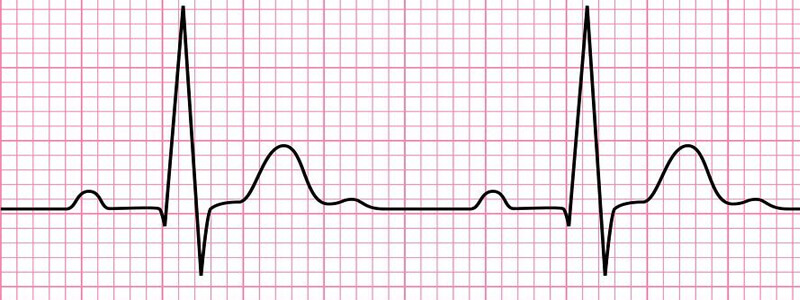
\includegraphics[scale=.]{image/week1/intro.jpg}
     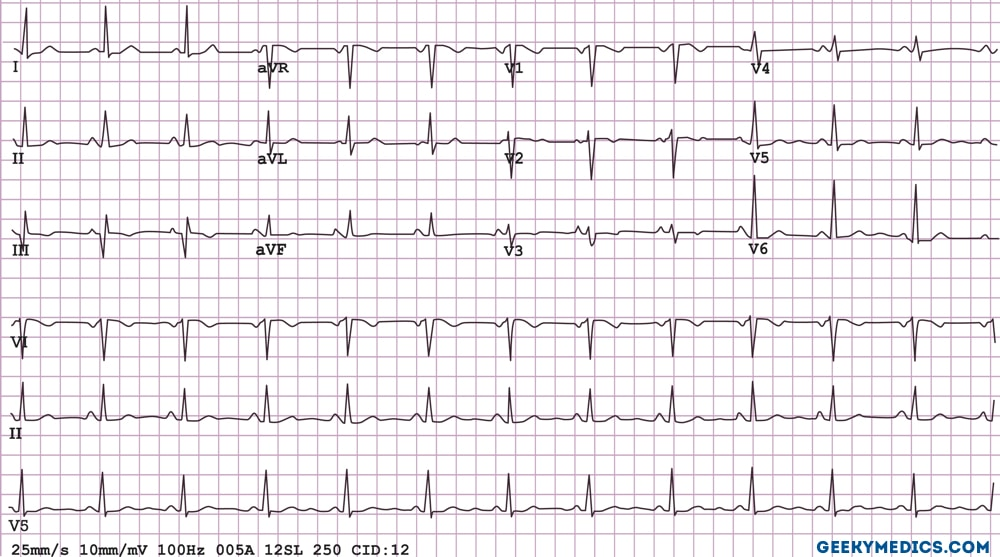
\includegraphics[scale=.35]{image/chapter1/Normal-ECG-SCALED-DOWN-WATERMARK.jpg}
    \end{center}
    \caption{Một đoạn điện tâm đồ }
    \end{figure}
\end{center}

\subsection{Lich sử hình thành điện tâm đồ}
\begin{itemize}
    \item 1887 - Augustus D. Waller (St Mary's Medical School, Luân Đôn) trình bày ECG đầu tiên trên người của Thomas Goswell, một người làm việc trong phòng thử nghiệm.
    \item 1893 - Willem Einthoven giới thiệu từ 'electrocardiogram' tại buổi họp của Hội Y Học Hà Lan (nhưng sau đó ông sửa lại rằng Waller là người đầu tiên dùng chữ này).
    \item 1895 - Einthoven cải tiến dụng cụ và công thức ghi điện, ghi được 5 thay đổi điện trong một nhịp tim, ông ghép chữ cho 5 thay đổi này (P, Q, R, S, T, U).
\end{itemize}

\subsection{Hoạt động điện của cơ tim và sự hình thành điện tâm đồ}
Do sự biến đổi hiệu thế giữa mặt trong và mặt ngoài màng tế bào cơ tim. Sự biến đổi hiệu thế này bắt nguồn từ sự di chuyển của các ion K + , Na + ,... từ ngoài vào trong tế bào và từ trong tế bào ra ngoài khi tế bào cơ tim hoạt động. Lúc này tính thẩm thấu của màng tế bào đối với các ion luôn luôn biến đổi. Do sự chênh lệch nồng độ hai bên màng tạo nên hiệu điện thế giữa hai bên màng (điện thế nghỉ).
\begin{center}
    \begin{figure}[htp]
    \begin{center}
     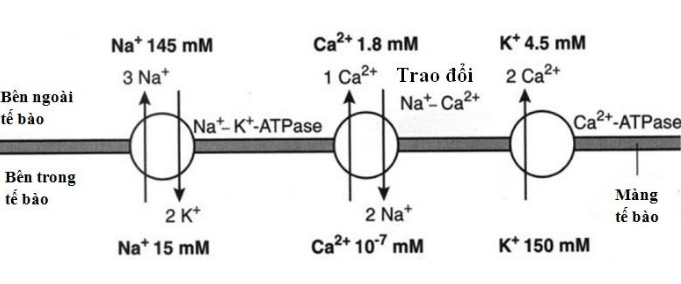
\includegraphics[scale=.4]{image/week1/h21.png}
    \end{center}
    \caption{Sự chênh lệch nồng độ của các ion Na, K, Ca trong cơ chế hình thành điện tâm đồ \cite{huongdanDTT}}
    \end{figure}
\end{center}\par
Tim người có 4 buồng để chứa và bơm máu. Hai phần nhỏ ở phía trên gọi là tâm nhĩ (vì trông giống lỗ tai). Hai phần dưới lớn hơn gọi là tâm thất. Máu theo tĩnh mạch từ cơ thể trở về tâm nhĩ phải, từ phổi trở về tâm nhĩ trái. Tâm nhĩ trái bóp bơm máu vào tâm thất trái, tâm nhĩ phải đưa máu vào tâm thất phải. Sau đó tâm thất phải bóp để bơm máu theo động mạch lên phổi và tâm thất trái bóp để bơm máu xuống cơ thể. Tim có khả năng hoạt động đều đặn và thứ tự như thế là nhờ một hệ thống các tế bào dẫn điện đặc biệt nằm trong cơ tim.\par
Trong tâm nhĩ bên phải có nút xoang nhĩ (sinoatrial node) gồm các tế bào có khả năng tự tạo xung điện (electric impulse). Xung điện này truyền ra các cơ chung quanh làm co bóp hai tâm nhĩ (tạo nên sóng P trên Điện Tâm đồ). Sau có dòng điện tiếp tục truyền theo 1 chuỗi tế bào đặc biệt tới nút nhĩ thất (atrioventricular node) nằm gần vách liên thất rồi theo chuỗi tế bào sợi Purkinje chạy dọc vách liên thất lan vào các cơ chung quanh (loạt sóng QRS) làm hai thất này co bóp. Sau đó xung điện giảm đi, tâm thất giãn ra (tạo nên sóng T).

\subsection{Các sóng cơ bản và sự hình thành phức bộ sóng}
Một chu kỳ tim biểu hiện trên điện tâm đồ là: sóng P, phức bộ QRS, sóng T, và sóng U (nếu có), hình dạng, thời gian kéo dài của sóng/phức bộ và cả thời gian giữa các thành phần với nhau đều có ý nghĩa đặc biệt quan trọng trong việc chẩn đoán.
\begin{center}
        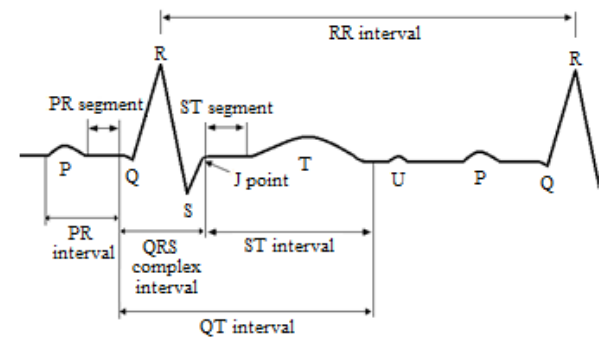
\includegraphics[scale=.4]{image/week1/h32.png}
        \begin{figure}[htp]
        \begin{center}
        \end{center}
        \caption{Tổng hợp những sóng cơ bản}
        \end{figure}
\end{center}

\subsubsection{Các sóng và phức bộ}
\textbf{Sóng P}\par
Sóng P hình thành do quá trình khử cực tâm nhĩ (cả nhĩ trái và nhĩ phải), bình thường biên độ của sóng P thường dưới 2mm (0.2mmV), và thời gian của sóng P là từ 0.08 đến 0.1 giây, việc tăng biên độ và kéo dài thời gian của sóng gợi ý đến một tình trạng tâm nhĩ lớn (tăng biên độ gợi ý lớn nhĩ phải. thời gian khử cực kéo dài gợi ý đến lớn nhĩ trái).\par
\textbf{Phức bộ QRS}\par
Phức bộ QRS thể hiện quá trình khử cực của tâm thất, tùy vào chiều khử cực và vị trí đặt điện cực mà trên giấy ghi sẽ cho thấy các phức bộ khác nhau, ưu thế sóng R hay S, bình thường QRS kéo dài từ 0.06 đến 0.1 giây.
\begin{itemize}
    \item Sóng Q là sóng âm đầu tiên của phức bộ QRS, sóng Q trên bệnh nhân bình thường thường nhỏ và ngắn (hình thành do quá trình khử cực vách liên thất), một sóng Q sâu (biên độ âm lớn) và kéo dài cho thấy một tình trạng hoại tử cơ tim (Trong nhồi máu cơ tim cũ hay nhồi máu cơ tim không có ST chênh lệch).
    \item Sóng R là sóng dương đầu tiên của phức bộ, và sóng âm sau nó là S, đây là hai sóng hình thành do khử cực thất, về bản chất là giống nhau, nếu điện cực đặt ở vị trị chiều khử cực hướng đến thì sóng R sẽ ưu thế, như trong chuyển đạo DII, V5, V6. Sóng R sẽ ưu thế hơn nếu chiều khử cực đi xa vị trí đặt điện cực như V1, V2.
\end{itemize}
\par
\textbf{Sóng T}\par
Là sóng theo sau phức bộ QRS, thể hiện quá trình tái cực muộn của 2 tâm thất, sóng T có giá trị rất lớn trong việc nhận định một tình trạng cơ tim thiếu máu.\par
\textbf{Sóng U}\par
Nguồn gốc sóng U vẫn chưa điện xác định rõ ràng, các giả thuyết đặt ra là:
\begin{itemize}
    \item Tái cực chậm sợi Purkinje.
    \item Tái cực kéo dài giữa cơ tim tế bào M (mid-myocardial cell).
    \item Sau kết quả điện thế của trương lực cơ trong các thành tâm thất.
\end{itemize}
Bình thường không thấy sóng U trên điện tâm đồ, nếu có thì là sóng nhỏ sau sóng T, sóng U đảo ngược hay nhô cao nhọn gặp trong rất nhiều loại bệnh lý tim (bệnh mạch vành, tăng huyết áp, bệnh van tim, tim bẩm sinh, bệnh lý cơ tim, cường giáp, ngộ độc, rối loạn điện giải,...)
\subsubsection{Các đoạn - khoảng}
\textbf{Khoảng PQ}\par
Là thời gian dẫn truyền từ nhĩ đến thất, bình thường từ 0.12 - 0.2 giây, việc kéo dài thể hiện quá trình chậm dẫn truyền (do bị block), PQ ngắn sẽ gợi ý đến một hội chứng kích thích sớm (Wolf-Parkinson-White)\par
\textbf{Đoạn ST}\par
Ý nghĩa là giai đoạn tái cực thất sớm, thời gian của ST thường không quan trọng bằng hình dạng của nó, bình thường ST nằm chênh lệch lên hoặc chênh xuống khỏi đường đẳng điện rất ít. đoạn ST cực kỳ quan trọng trong việc chẩn đoán nhồi máu cơ tim.\par
ST gọi là chênh lệch nếu cao hơn đường đẳng điện 1mm ở chuyển đạo chi và hơn 2mm ở chuyển đạo trước ngực\par
ST gọi là chênh xuống khi nằm dưới đường đẳng điện hơn 0.5mm\par
\textbf{Đoạn QT}\par
Là thời gian tâm thu điện học của tâm thất, khoảng giá trị bình thường của QT phục thuộc vào tần số tim, QT kéo dài bất thường có liên quan với tăng nguy cơ loạn nhịp thất, đặc biệt là xoắn đỉnh. Gần đây, hội chứng QT ngắn bẩm sinh đã được tìm thấy có liên quan với tăng nguy cơ rung nhĩ và thất kịch phát và đột tử do tim.

\subsection{Các chuyển đạo thông dụng}

\subsubsection{Điện trường tim}
Cơ thể con người là một môi trường dẫn điện; vì thế, dòng điện do tim phát ra được dẫn truyền khắp cơ thể, ra tới da, biến cơ thể thành một điện trường của tim. Nếu ta đặt hai điện cực lên bất cứ hai điểm nào đó có điện thế khác nhau của điện trường đó, ta sẽ thu được một dòng điện thể hiện hiệu thế giữa hai điểm đó và gọi là một chuyển đạo hay đạo trình (lead). Nó hiện ra trên máy ghi bằng một đường cong điện tâm đồ có một hình dạng nào đó tùy theo địa điểm đặt các điện cực. Đường thẳng nối hai địa điểm đặt điện cực trên cơ thể gọi là trục chuyển đạo.

\subsubsection{Chuyển đạo mẩu:}
\begin{center}
    \begin{figure}[htp]
    \begin{center}
    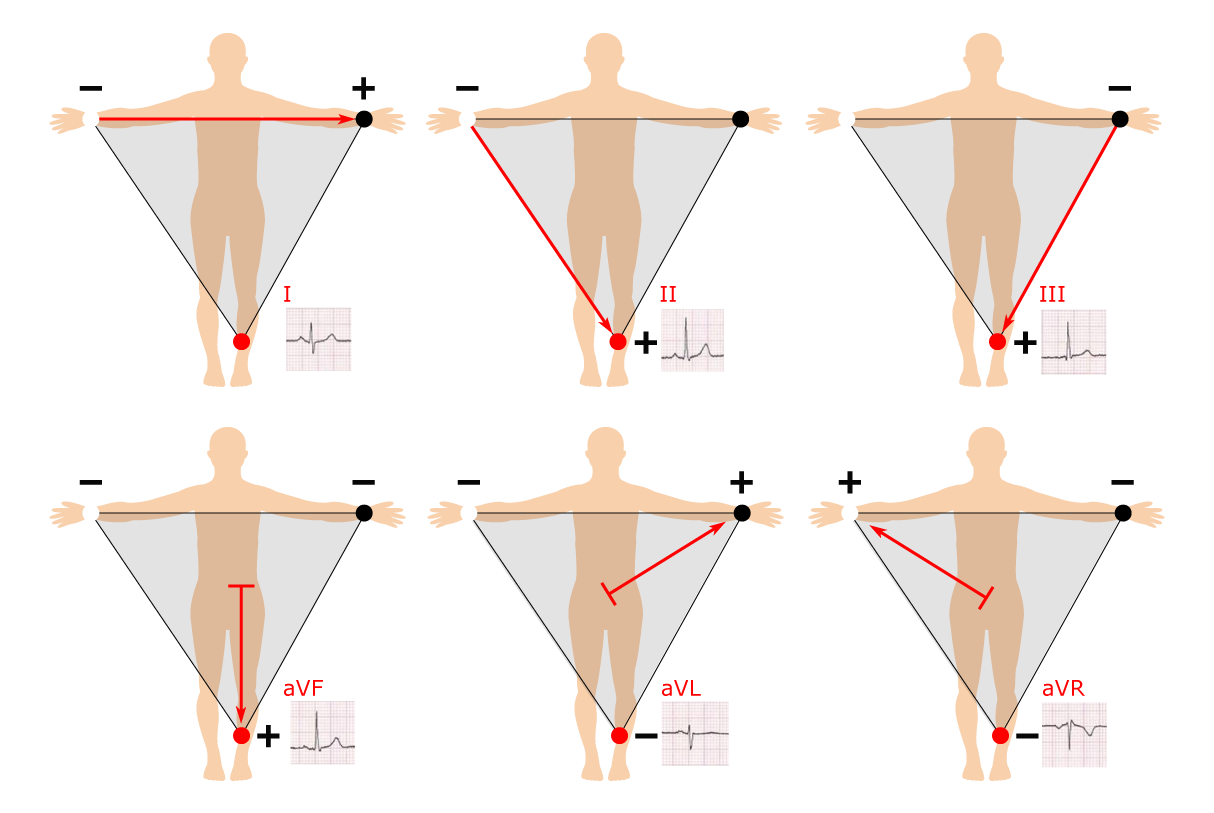
\includegraphics[scale=.2]{image/week1/chuyendaochi.png}
    \end{center}
    \caption{Chuyển đạo chi \cite{chuyendao}}
    \end{figure}
\end{center}
Tất cả 6 chuyển đạo: D1, D2, D3, aVR, aVL, aVF được gọi chung là các chuyển đạo ngoại biên vì đều có điện cực thăm dò đặt ở các chi. Chúng hỗ trợ cho nhau “dò xét” các rối loạn của dòng điện tim thể hiện ở bốn phía xung quanh quả tim trên mặt phẳng chắn (frontal plane).
\begin{center}
    \begin{figure}[htp]
    \begin{center}
    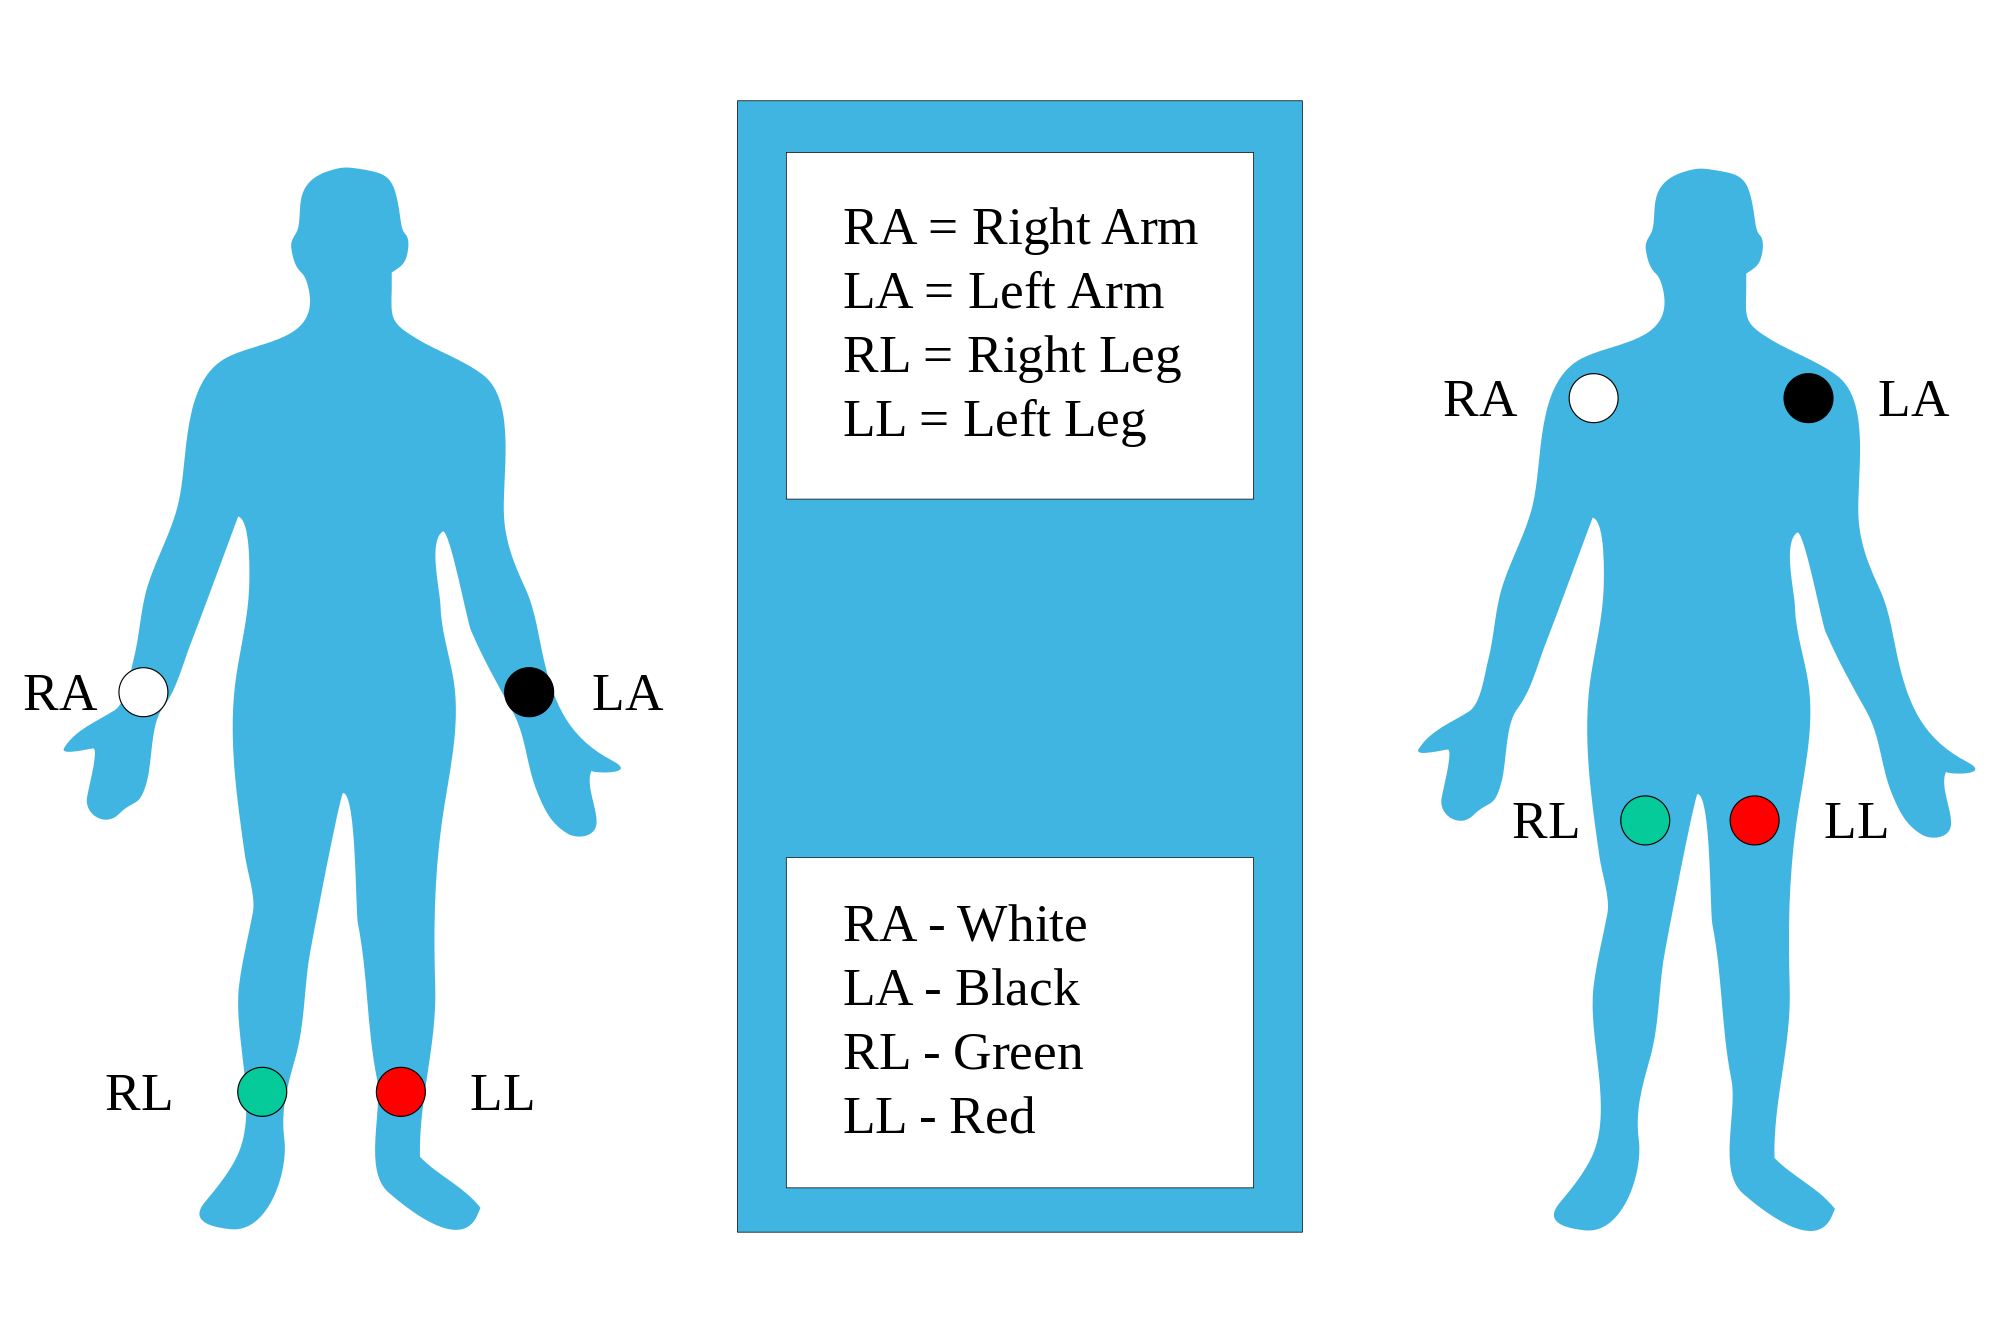
\includegraphics[scale=.12]{image/chapter1/2000px-Limb_leads.png}
    \end{center}
    \caption{Các vị trí đặt điện cực để đo ECG}
    \end{figure}
\end{center}

\subsubsection{Chuyển đạo trước tim:}
\begin{center}
    \begin{figure}[htp]
    \begin{center}
    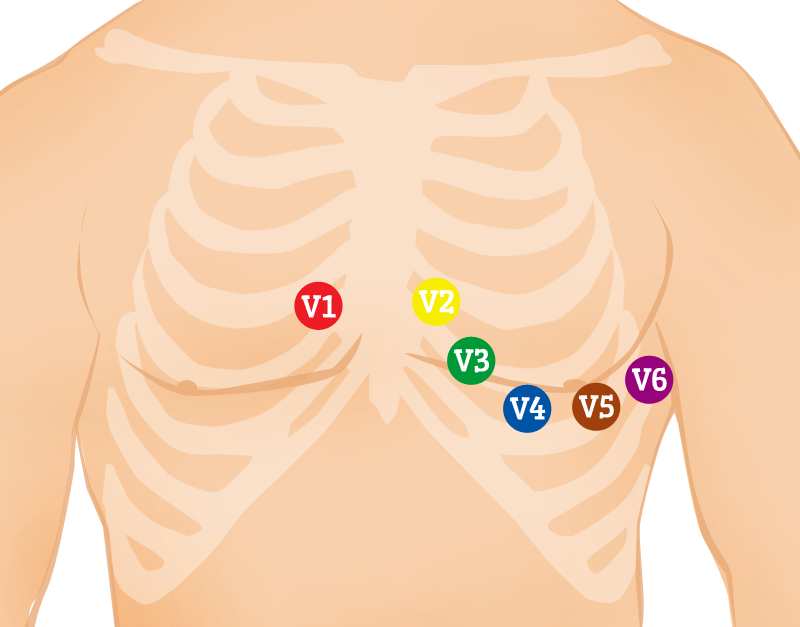
\includegraphics[scale=.25]{image/week1/chuyendaotruocnguc.png}
    \end{center}
    \caption{Chuyển đạo trước tim }
    \end{figure}
\end{center}
Người ta thường ghi đồng loạt cho bệnh nhân 6 chuyển đạo trước tim thông dụng nhất, kí hiệu bằng chữ V (voltage) kèm theo các chỉ số từ 1 đến 6.(V1, V2,…,V6).

\subsubsection{Một số chuyển đạo khác:}
V7, V8, V9(điện cực ở mé trái và sau lồng ngực dùng để thăm dò thất trái), V3R, V4R, V5R, V6R(điện cực ở mé phải lồng ngực dùng để nghiên cứu thất phải hay tim sang phải), chuyển đạo thực quản (Kí hiệu VOE), chuyển đạo trong buồng tim, điện đồ His.

\subsection{Đo điện tâm đồ}
\subsubsection{Đo điện tâm đồ truyền thống}
Định dạng chuẩn của một điện tâm đồ là điện tâm đồ được ghi lại trên một khổ giấy
.Để đánh giá thời gian dài hay ngắn và biên độ cao hay thấp của các làn sóng điện tâm đồ, người ta đinh chuẩn: 
\begin{itemize}
    \item Vận tốc 25mm/s thì mỗi ô 1mm có giá trị 0,04s.
    \item Theo chiều ngang 1 ô lớn tương ứng với 1000ms.
    \item Theo chiều dọc 1 ô lớn tương ứng 500mV.
\end{itemize}
\begin{center}
    \begin{figure}[htp]
    \begin{center}
    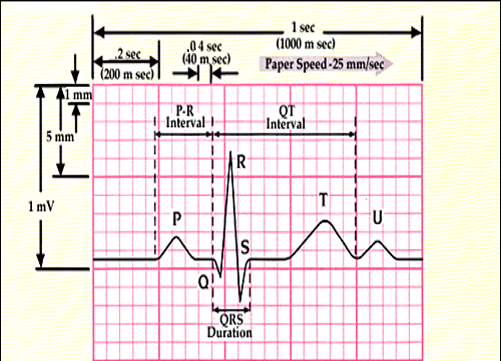
\includegraphics[scale=.6]{image/week1/new_ecg_paper.png}
    \end{center}
    \caption{Hình ảnh một chu kỳ sóng được đo theo kích thước khổ giấy, bác sĩ căn cứ vào ô trên giấy để phát hiện bất thường ở ECG \cite{ecggiay}}
    \end{figure}
\end{center}
\subsubsection{Đo điện tâm đồ bằng thiết bị di động thông minh (Apple Watch Series 4)}
Tính năng ECG hay còn gọi là đo điện tâm đồ đã chính thức có thể sử dụng trên Apple Watch Series 4 để phát hiện nhịp tim bất thường và chẩn đoán các bệnh tim nghiêm trọng.
\begin{center}
    \begin{figure}[htp]
    \begin{center}
    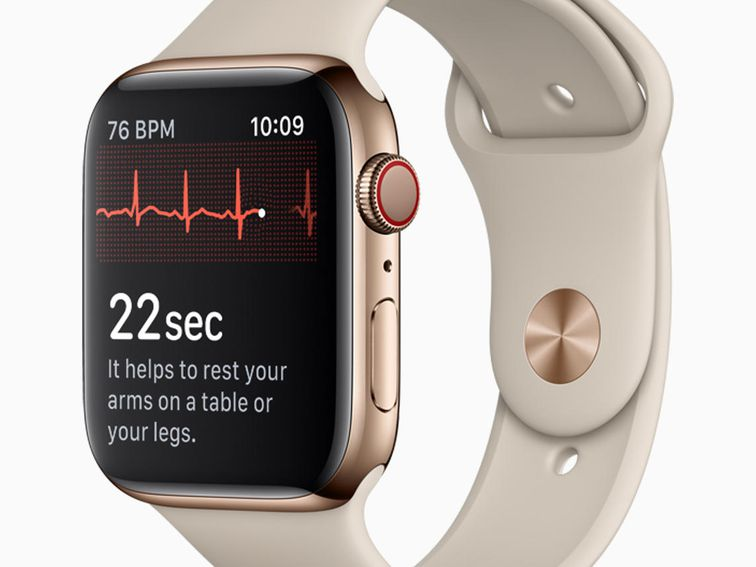
\includegraphics[scale=.3]{image/chapter1/apple-watch-series4-ecg-crown-09122018.jpg}
    \end{center}
    \caption{Apple Watch Series 4}
    \end{figure}
\end{center}
% \section{Đọc một điện tâm đồ}
% \subsection{Những bước phân tích trước khi đọc một điện tâm đồ}
% Điện tâm đồ (ECG) là một đường cong ghi lại các biến thiên của các điện lực do tim phát ra trong khi hoạt động co bóp.\cite{huongdanDTT}

% \begin{enumerate}
%     \item Trước khi đọc điện tâm đồ, phải nắm vững tuổi, giới tính, chẩn đoán lâm sàng của bệnh
%     nhân. Ngoài ra, còn nên biết thêm sơ lược bệnh án, hình ảnh X quang, các kết quả xét nghiệm khác và nhất là hai vấn đề sau đây:
%     \begin{itemize}
%         \item Khổ người bệnh nhân gầy béo, cao thấp ảnh hưởng rất nhiều đến tư thế tìm và biên độ sóng, nó ảnh hưởng nhiều đến chẩn đoán dày thất.
%         \item Có đang dùng thuốc trợ tim hay thuốc chống loạn nhịp dài ngày không? Nhất là digitan và quinidin… vì các thuốc này tác động rất nhiều đến hình dạng điện tâm đồ và dễ làm sai lạc chẩn đoán cơ bản.
%     \end{itemize}
%     \item Kiểm tra kỹ thuật ghi điện tâm đồ, phát hiện ghi sai, ảnh hưởng tạp, milivôn lấy đúng 1cm
%     hay không? Tốc độ ghi bao nhiêu? Nghĩa là các đường kẻ dọc cách nhau bao nhiêu phần trăm
%     giây
%     \item Nhịp tim: bước vào đọc điện tâm đồ trước hết bao giờ cũng phải xem nhịp xoang hay
%     không xoang? Có những rối loạn nhịp tim gì? Đừng bao giờ quên tính tần số tim. Nếu có blốc
%     nhĩ-thất thì phải tính riêng cả tần số nhĩ.
%     \item Trục điện tim với góc alpha, tư thế tim.
%     \item Hình dạng các sóng: đọc đồng thời ở cả 12 chuyển đạo thông dụng:
%     \begin{itemize}
%         \item Sóng P: chiều cao (biên độ), chiều rộng (thời gian), hình dạng (âm, dương, hai pha, móc).
%         \item Khoảng PQ dài bao nhiêu?
%         \item Phức bộ QRS: biên độ và thời gian chung và riêng của sóng Q, hình dạng (móc…).
%         \item Riêng với V1 và V5 thì tìm thêm thời gian xuất hiện nhánh nội điện.
%         \item Đoạn ST có chênh không?
%         \item Sóng T (và sóng U): dạng (dương, âm hay hai pha), biên độ.
%         \item Khoảng QT dài bao nhiêu?
%     \end{itemize}
%     \item Kết luận chẩn đoán: về tổn thương cơ tim và về rối loạn nhịp tim.
% \end{enumerate}

% \chapter{Dữ liệu về điện tim}
\newpage

\section{Physionet}
\subsection{Thông tin về dataset}
Là một trang web truy cập miễn phí các bộ dữ liệu lớn về tín hiệu sinh lý được ghi lại (PhysioBank) và những phần mềm mã nguồn mở liên quan (PhysioToolkit).
\begin{center}
    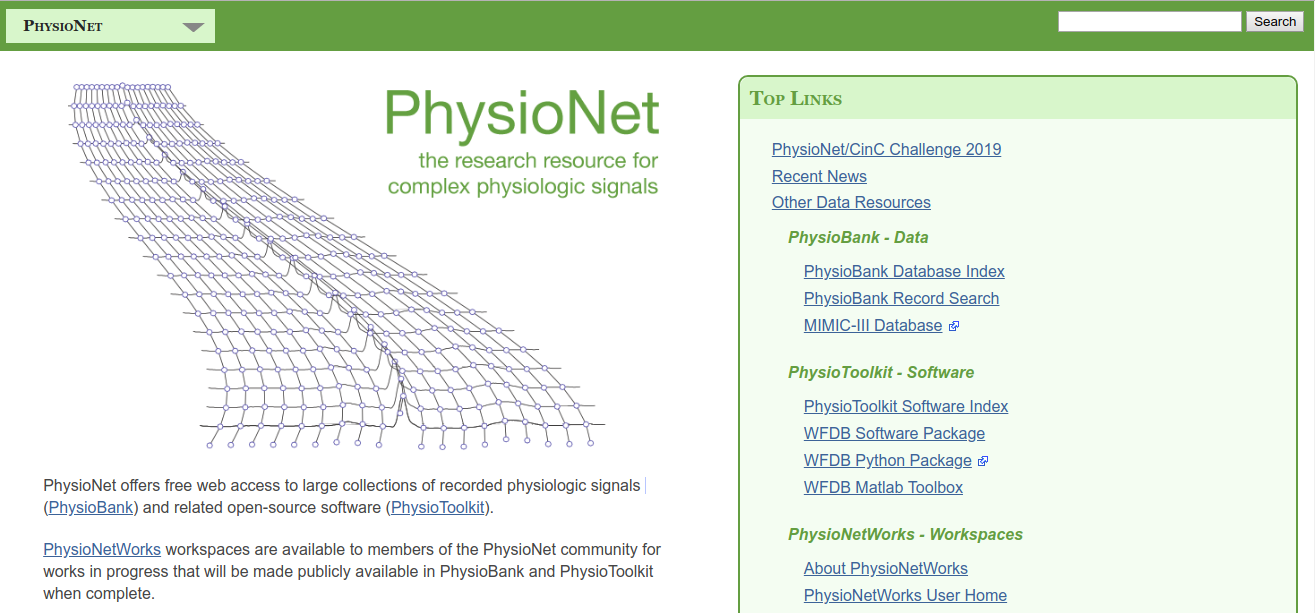
\includegraphics[scale=.3]{image/chapter3/Screenshot_from_2019-03-11_04-58-18.png}
    \begin{figure}[htp]
    \begin{center}
    \end{center}
    \caption{Trang Physionet}
    \end{figure}
\end{center}

\subsection{MIT-BIH Arrhythmia Database}
\textbf{Thông tin về database}
Đây là bộ dữ liệu nổi tiếng nhất, nhiều bài báo cũng như nghiên cứu dựa trên bộ dữ liệu này. Tập dữ liệu bao gồm 48 file. Mỗi file gồm: 1 file dat chứa dữ liệu, một file atr chứa chú thích, 1 file hea chứa header.
\begin{center}
    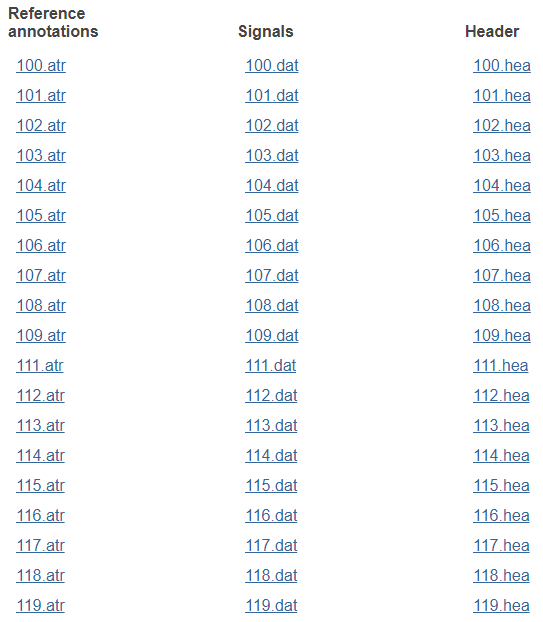
\includegraphics[scale=.4]{image/week3/mit.png}
    \begin{figure}[htp]
    \begin{center}
    \end{center}
    \caption{Dataset sample}
    \end{figure}
\end{center}
Phân tích và plot file 100.mat thành đồ thị.
\begin{center}
    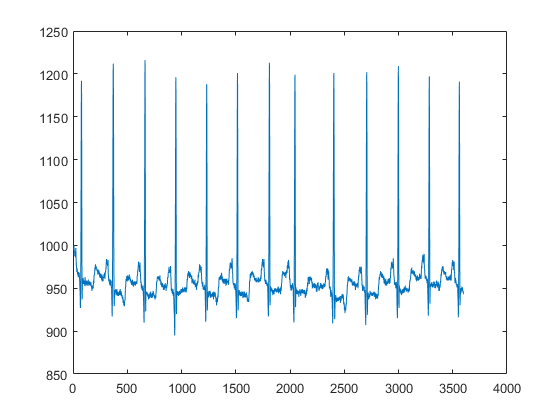
\includegraphics[scale=.8]{image/week4/100dat.png}
    \begin{figure}[htp]
    \begin{center}
    \end{center}
    \caption{100.mat sau khi plot thành đồ thị thể hiện hình dạng ECG}
    \end{figure}
\end{center}

% \chapter{Tìm hiểu một số nghiên cứu về phân loại điện tâm đồ bằng Deep Learning}

\section{Xác định hình dạng sóng}
-Nhiều phương pháp được sử dụng qua nhiều nghiên cứu để tìm ra các đối tượng trong ECG \cite{realtimeQRS} \cite{concho}, Một trong những phương pháp quan trọng đó là sử dụng wavelet transform.\par
-Trong nghiên cứu \cite{4} tác giả tìm đoạn QRS và RR interval bằng cách sử dụng Slope Vector WaveForm.\par
-Nhiều giải thuật được đề xuất trong suốt 20 năm bởi vì tầm quan trọng của xác định đoạn QRS trong phân tích ECG. Những giải thuật được dùng như: filter bank, neural network, wavelet transform và những giải thuật khác được thực hiện \cite{5}. Chủ yếu là linear và unlinear filters được dùng để xác định \cite{6}.\par
-Trong nghiên cứu \cite{7} cubic spline wavelet được dùng để xác định QRS với độ chính xác rất cao.\par
-Trong nghiên cứu \cite{8} 2 phương pháp được dùng là postprocessing và preprocessing để xác định QRS và loại bỏ noise trong tín hiệu ECG. Đầu tiên preprocessing được dùng để xác định nhịp QRS bằng cách sử dụng threshhold, 4 loại threshold khác nhau được sử  dụng ở phần này. Tiếp theo, postprocessing được dùng để loại bỏ nhiễu xuất hiện ở đoạn sóng R.\par
-Trong nghiên cứu \cite{9}, sóng QRS được xác định bằng kỹ thuật dự đoán đệ quy thời gian. Được sử dụng để xác định sóng QRS ở lead 1 và lead 3.\par
-Trong nghiên cứu \cite{10} ngôn ngữ Z80 assembly được đề xuất để xác định QRS theo thời gian thực.
\section{Phân loại điện tim}
-Trong nghiên cứu \cite{11}, phân loại điện tim dựa trên Neural Network và Fuzzy.par
-Trong nghiên cứu \cite{12}, sự khác nhau giữa sóng bình thường được phân loại bằng cách sử dụng (Linear Discriminant Analysis) LDA and Artificial Neural Networks (ANN). Một số nghiên cứu cho thấy MLP (Multilayer Perception) được dùng trong ANN tốt hơn phân loại LDA. MLP trong ANN được sử dụng để tìm bình thường và bất thường ở ở nhịp tim.\par
-Principal component analysis (PCA) và một số cấu trúc neural network được sử dụng và phân loại điện tim. Kết quả của việc này là để tìm ra mô hình neural network phù hợp nhất cho từng loại loạn nhịp khác nhau.\par
-Trong nghiên cứu \cite{13}, để thu giảm chiều dữ liệu bằng PCA. Bài báo này đã kết hợp các giải thuật phân cụm giữa FCA và PCA neural networ, và đã chứng minh sự kết hợp này tốt hơn là sử dụng riêng lẻ. Sự so sánh giữa các giải thuật xác định loạn nhịp tim được sử dụng trong nghiên cứu \cite{14}. Trong đó KNN cũng được sử dụng để xác định QRS\par.
-Trong nghiên cứu \cite{rnn}, Shraddha Singh và nhóm nghiên cứu đã phân loại ECG bằng mạng Neuron hồi quy và các biến thể để phân loại điện tim.\par
-Trong nghiên cứu \cite{mohinhchinh}, Trần Thanh Duy và nhóm nghiên cứu đã dùng Vital Sign Holter để thu thập dữ liệu điện tim, sử dụng mạng Autoencoder để thu giảm chiều dữ liệu và mạng LSTM để phân lại điện tim.


% \chapter{Những kiến thức nền tảng trong một mô hình phát hiện bất thường ở điện tâm đồ}
\newpage

\section{Kỹ thuật lọc nhiễu Butterworth}
Bộ lọc Butterworth là một loại bộ lọc xử lý tín hiệu được thiết kế để có đáp ứng tần số càng phẳng càng tốt trong băng thông. Nó cũng được gọi là một bộ lọc cường độ phẳng tối đa. Nó được mô tả lần đầu tiên vào năm 1930 bởi kỹ sư và nhà vật lý người Anh Stephen Butterworth trong bài báo của ông có tựa đề "Về lý thuyết của bộ khuếch đại bộ lọc".
\section{Kỹ thuật ngưỡng kích ứng thích hợp}

\section{Mạng Neural Hồi quy (RNN)}
\subsection{Giới thiệu}
Con người không bắt đầu suy nghĩ của họ từ đầu tại tất cả các thời điểm. Cũng như bạn đang đọc bài viết này, bạn hiểu mỗi chữ ở đây dựa vào từ bạn đã hiểu các chữ trước đó chứ không phải là đọc tới đâu ném hết đi tới đó, rồi lại bắt đầu suy nghĩ lại từ đầu tới chữ bạn đang đọc. Tức là tư duy đã có một bộ nhớ để lưu lại những gì diễn ra trước đó.\\
Tuy nhiên các mô hình mạng nơ-ron truyền thống thì không thể làm được việc đó, đó có thể coi là một khuyết điểm chính của mạng nơ-ron truyền thống. Ví dụ, bạn muốn phân loại các bối cảnh xảy ra ở tất cả các thời điểm trong một bộ phim, thì đúng là không rõ làm thế nào để có thể hiểu được một tình huống trong phim mà lại phụ thuộc vào các tình huống trước đó nếu sử dụng các mạng nơ-ron truyền thống.\\
Mạng nơ-ron hồi quy (Recurrent Neural Network) sinh ra để giải quyết vấn đề đó. Mạng này chứa các vòng lặp bên trong cho phép thông tin có thể lưu lại được.
\begin{center}
    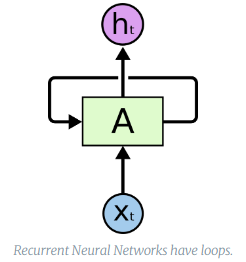
\includegraphics[scale=.5]{image/chapter6/RNN-node.png}
    \begin{figure}[htp]
    \begin{center}
    \end{center}
    \caption{một đoạn của mạng nơ-ron hồi quy A với đầu vào là $x_{n}$ và đầu ra là $h_{t}$. Một vòng lặp cho phép thông tin có thể được truyền từ bước này qua bước này qua bước khác của mạng nơ-ron. \cite{rnn-basic}}
    \end{figure}
\end{center}
Một mạng nơ-ron hồi quy có thể được coi là nhiều bản sao chép của cùng một mạng, trong đó mỗi đầu ra của mạng này là đầu vào của một mạng sao chép khác.\par
\begin{center}
    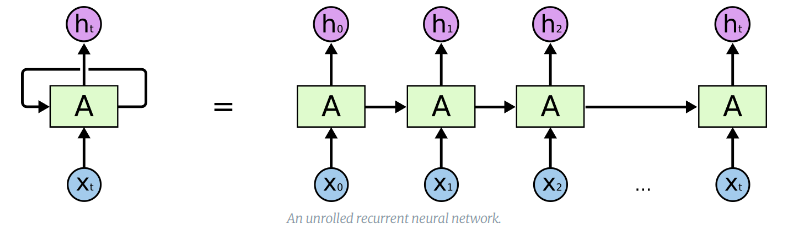
\includegraphics[scale=.5]{image/chapter6/RNN-ab.png}
    \begin{figure}[htp]
    \begin{center}
     
    \end{center}
    \caption{Chuỗi lặp lại các mạng này chính là phân giải của mạng nơ-ron hồi quy, các vòng lặp khiến chúng tạo thành một chuỗi danh sách các mạng sao chép nhau. \cite{rnn-basic}}
    \end{figure}
\end{center}
Một cách chi tiết hơn.
\begin{center}
    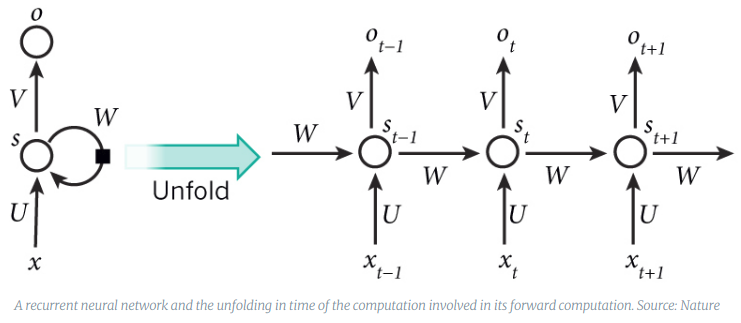
\includegraphics[scale=.4]{image/chapter6/rnn-detail.png}
    \begin{figure}[htp]
    \begin{center}
     
    \end{center}
    \caption{Chi tiết mạng RNN \cite{rnn-basic}}
    \end{figure}
\end{center}
\begin{itemize}
    \item $x_{t}$ là đầu vào tại bước t.
    \item $s_{t}$ là trạng thái ẩn tại bước t. Nó chính là bộ nhớ của mạng. $s_{t}$ được tính toán dựa trên cả các trạng thái ẩn phía trước và đầu vào tại bước đó: $s_{t} = f(Ux_{t}+Ws_{t-1})$. Hàm $f$ thường là một hàm phi tuyến như tang hyperbolic (tanh) hay Relu. Để làm phép toán cho phần tử ẩn đầu tiên ta cần khởi tạo thêm $s_{-1}$, thường giá trị khởi tạo được gắn bằng 0.
    \item $o_{t}$ là đầu ra tại bước t. Ví dụ, ta muốn dự đoán từ tiếp theo có thể xuất hiện trong câu thì $o_{t}$ chính là một vec-tơ xác xuất các từ trong danh sách từ vựng của ta: $o_{t} = softmax(Vs_{t})$. 
\end{itemize}


\subsection{Một số ứng dụng của RNN}
\begin{itemize}
    \item Nhận dạng giọng nói: Đưa vào một chuỗi các tín hiệu âm thanh, ta có thể dự đoán được chuỗi các đoạn ngữ âm đi kèm với xác xuất của chúng.
    \item Mô tả hình ảnh: Cùng với ConvNet, RNN được sử dụng để tự động tạo mô tả cho các ảnh chưa được gán nhãn. Sự kết hợp này đã đưa ra được các kết quả khá kinh ngạc. Ví dụ như các ảnh dưới đây, các mô tả sinh ra có mức độ chính xác và độ tường tận khá cao.
    \begin{center}
    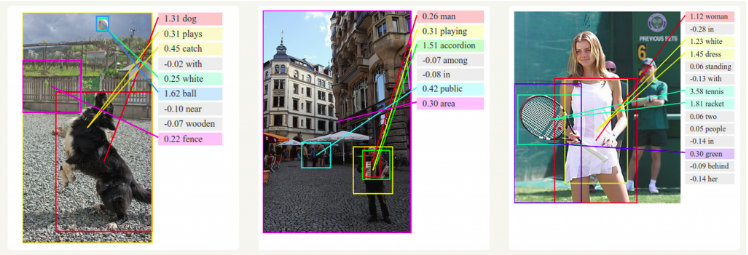
\includegraphics[scale=.4]{image/chapter6/RNN-application.png}
    \begin{figure}[htp]
    \begin{center}
     
    \end{center}
    \caption{Ứng dụng của RNN trong phân loại ảnh \cite{rnn-basic}}
    \end{figure}
    \end{center}
\end{itemize}


\subsection{RNN mở rộng}
\begin{itemize}
    \item RNN 2 chiều: Ở mô hình RNN 2 chiều (Bidirectional RNN), đầu ra tại bước t không những phụ thuộc vào các phần tử phía trước mà còn phụ thuộc cả vào các phần tử phía sau. Ví dụ, để dự đoán từ còn thiếu trong câu, thì việc xem xét cả phần trước và phần sau của câu là cần thiết. Vì vậy, ta có thể coi mô hình là việc chồng 2 mạng RNN ngược hướng nhau lên nhau. Lúc này đầu ra được tính toán dựa vào cả 2 trạng thái ẩn của 2 mạng RNN ngược hướng này.
    \begin{center}
    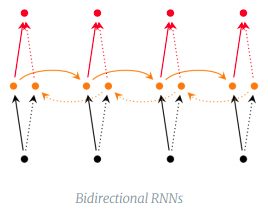
\includegraphics[scale=.5]{image/chapter6/RNN-2.png}
    \begin{figure}[htp]
    \begin{center}
     
    \end{center}
    \caption{RNN 2 chiều \cite{rnn-basic}}
    \end{figure}
    \end{center}
    \item RNN (2 chiều) sâu: RNN sâu (Deep (Bidirectional) RNN) cũng tương tự như RNN 2 chiều, nhưng khác nhau ở chỗ chúng chứa nhiều tầng ẩn ở mỗi bước. Trong thực tế, chúng giúp cho việc học ở mức độ cao hơn, tuy nhiên ta cũng cần phải có nhiều dữ liệu huấn luyện hơn.
    \begin{center}
    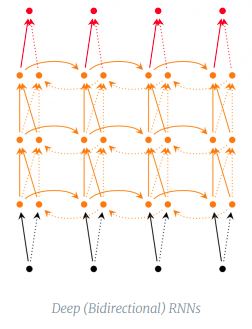
\includegraphics[scale=.3]{image/chapter6/RNN-4.png}
    \begin{figure}[htp]
    \begin{center}
     
    \end{center}
    \caption{RNN sâu \cite{rnn-basic}}
    \end{figure}
    \end{center}
\end{itemize}


\section{Mạng bộ nhớ ngắn dài (LSTM)}
\subsection{Vấn đề phụ thuộc xa}
Một điểm nổi bật của RNN chính là ý tưởng kết nối các thông tin phía trước để dự đoán cho hiện tại. Việc này tương tự như ta sử dụng các cảnh trước của bộ phim để hiểu được cảnh hiện thời. Nếu mà RNN có thể làm được việc đó thì chúng sẽ cực kì hữu dụng, tuy nhiên liệu chúng có thể làm được không? Câu trả lời là còn tùy.\\
Đôi lúc ta chỉ cần xem lại thông tin vừa có thôi là đủ để biết được tình huống hiện tại. Ví dụ, ta có câu: “các đám may trên bầu trời” thì ta chỉ cần đọc tới “các đám may trên bầu” là đủ biết được chữ tiếp theo là “trời” rồi. Trong tình huống này, khoảng cách tới thông tin có được cần để dự đoán là nhỏ, nên RNN hoàn toàn có thể học được.
\begin{center}
    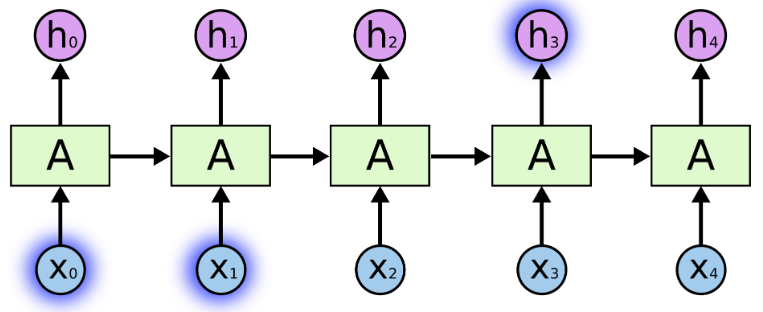
\includegraphics[scale=.3]{image/chapter6/ptx1.png}
    \begin{figure}[htp]
    \begin{center}
     
    \end{center}
    \end{figure}
\end{center}
Nhưng trong nhiều tình huống ta buộc phải sử dụng nhiều ngữ cảnh hơn để suy luận. Ví dụ, dự đoán chữ cuối cùng trong đoạn: “I grew up in France… I speak fluent French.”. Rõ ràng là các thông tin gần (”I speak fluent”) chỉ có phép ta biết được đằng sau nó sẽ là tên của một ngôn ngữ nào đó, còn không thể nào biết được đó là tiếng gì. Muốn biết là tiếng gì, thì ta cần phải có thêm ngữ cảnh “I grew up in France” nữa mới có thể suy luận được. Rõ ràng là khoảng cách thông tin lúc này có thể đã khá xa rồi.\\
Thật không may là với khoảng cách càng lớn dần thì RNN bắt đầu không thể nhớ và học được nữa.
\begin{center}
    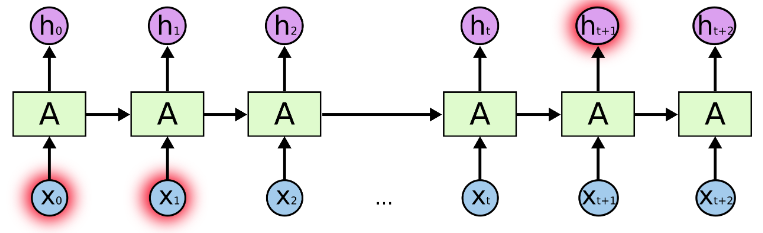
\includegraphics[scale=.3]{image/chapter6/ptx2.png}
    \begin{figure}[htp]
    \begin{center}
     
    \end{center}
    \end{figure}
\end{center}
Về mặt lý thuyết, rõ ràng là RNN có khả năng xử lý các phụ thuộc xa (long-term dependencies). Chúng ta có thể xem xét và cài đặt các tham số sao cho khéo là có thể giải quyết được vấn đề này. Tuy nhiên, đáng tiếc trong thực tế RNN có vẻ không thể học được các tham số đó. Vấn đề này đã được khám phá khá sâu bởi Hochreiter (1991) [tiếng Đức] và Bengio, et al. (1994), trong các bài báo của mình, họ đã tìm được nhưng lý do căn bản để giải thích tại sao RNN không thể học được.


\subsection{Mạng LSTM}
Mạng bộ nhớ dài-ngắn (Long Short Term Memory networks), thường được gọi là LSTM - là một dạng đặc biệt của RNN, nó có khả năng học được các phụ thuộc xa. LSTM được giới thiệu bởi Hochreiter và Schmidhuber (1997), và sau đó đã được cải tiến và phổ biến bởi rất nhiều người trong ngành. Chúng hoạt động cực kì hiệu quả trên nhiều bài toán khác nhau nên dần đã trở nên phổ biến như hiện nay.\\
LSTM được thiết kế để tránh được vấn đề phụ thuộc xa (long-term dependency). Việc nhớ thông tin trong suốt thời gian dài là đặc tính mặc định của chúng, chứ ta không cần phải huấn luyện nó để có thể nhớ được. Tức là ngay nội tại của nó đã có thể ghi nhớ được mà không cần bất kì can thiệp nào.\\
Mọi mạng hồi quy đều có dạng là một chuỗi các mô-đun lặp đi lặp lại của mạng nơ-ron. Với mạng RNN chuẩn, các mô-dun này có cấu trúc rất đơn giản, thường là một tầng $tanh$
\begin{center}
    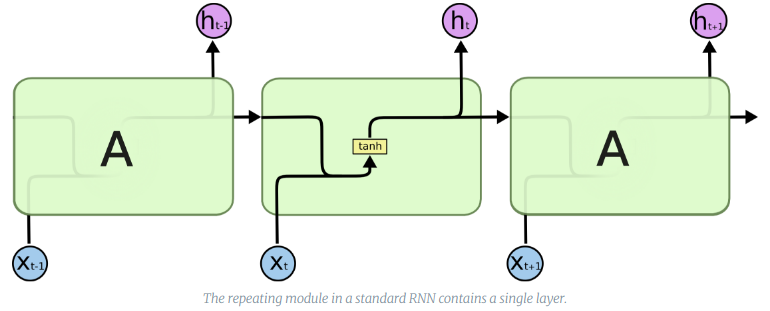
\includegraphics[scale=.3]{image/chapter6/lstm1.png}
    \begin{figure}[htp]
    \begin{center}
    \end{center}
    \end{figure}
\end{center}
LSTM cũng có kiến trúc dạng chuỗi như vậy, nhưng các mô-đun trong nó có cấu trúc khác với mạng RNN chuẩn. Thay vì chỉ có một tầng mạng nơ-ron, chúng có tới 4 tầng tương tác với nhau một cách rất đặc biệt.
\begin{center}
    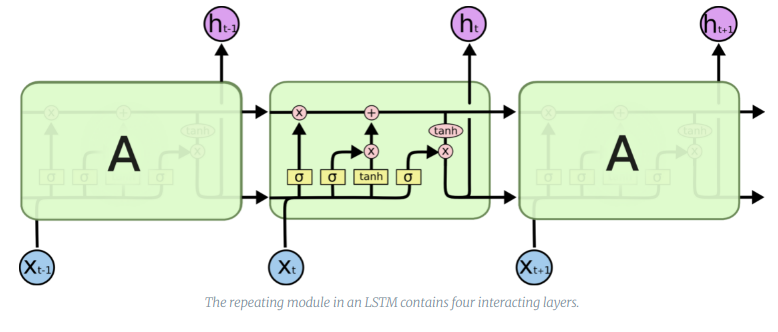
\includegraphics[scale=.3]{image/chapter6/lstm2.png}
    \begin{figure}[htp]
    \begin{center}
     
    \end{center}
    \end{figure}
\end{center}
Giờ thì đừng hoang mang về chi tiết bên trong chúng ngay, chúng ta sẽ khám phá chúng chi tiết chúng ở bước sau. Điều bạn cần làm bây giờ là làm hãy làm quen với các kí hiệu mà ta sẽ sử dụng ở dưới đây:
\begin{center}
    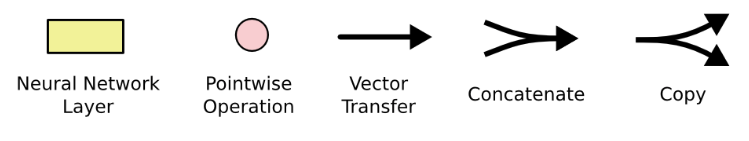
\includegraphics[scale=.3]{image/chapter6/lstm3.png}
    \begin{figure}[htp]
    \begin{center}
     
    \end{center}
    \end{figure}
\end{center}
Ở sơ đồ trên, mỗi một đường mang một véc-tơ từ đầu ra của một nút tới đầu vào của một nút khác. Các hình trong màu hồng biểu diễn các phép toán như phép cộng véc-tơ chẳng hạn, còn các ô màu vàng được sử dụng để học trong các từng mạng nơ-ron. Các đường hợp nhau kí hiệu việc kết hợp, còn các đường rẽ nhánh ám chỉ nội dung của nó được sao chép và chuyển tới các nơi khác nhau.


\subsection{Ý tưởng cốt lõi của LSTM}
Chìa khóa của LSTM là trạng thái tế bào (cell state) - chính đường chạy thông ngang phía trên của sơ đồ hình vẽ.\par
Trạng thái tế bào là một dạng giống như băng truyền. Nó chạy xuyên suốt tất cả các mắt xích (các nút mạng) và chỉ tương tác tuyến tính đôi chút. Vì vậy mà các thông tin có thể dễ dàng truyền đi thông suốt mà không sợ bị thay đổi.
\begin{center}
    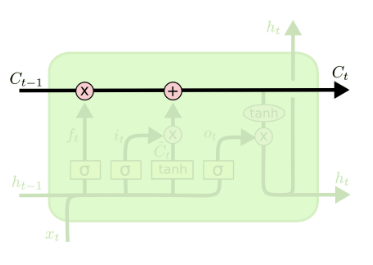
\includegraphics[scale=.5]{image/chapter6/yn1.png}
    \begin{figure}[htp]
    \begin{center}
     
    \end{center}
    \end{figure}
\end{center}
LSTM có khả năng bỏ đi hoặc thêm vào các thông tin cần thiết cho trạng thái tế báo, chúng được điều chỉnh cẩn thận bởi các nhóm được gọi là cổng (gate).\par
Các cổng là nơi sàng lọc thông tin đi qua nó, chúng được kết hợp bởi một tầng mạng sigmoid và một phép nhân.
\begin{center}
    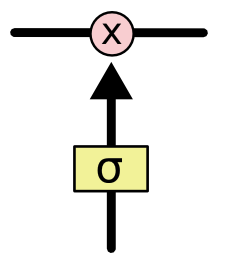
\includegraphics[scale=.3]{image/chapter6/yn2.png}
    \begin{figure}[htp]
    \begin{center}
     
    \end{center}
    \end{figure}
\end{center}
Tầng sigmoid sẽ cho đầu ra là một số trong khoản [0,1], mô tả có bao nhiêu thông tin có thể được thông qua. Khi đầu ra là 0 thì có nghĩa là không cho thông tin nào qua cả, còn khi là 1 thì có nghĩa là cho tất cả các thông tin đi qua nó.\\
Một LSTM gồm có 3 cổng như vậy để duy trì và điều hành trạng thái của tế bào.
\subsection{Bên trong LSTM}
Bước đầu tiên của LSTM là quyết định xem thông tin nào cần bỏ đi từ trạng thái tế bào. Quyết định này được đưa ra bởi tầng sigmoid - gọi là “tầng cổng quên” (forget gate layer). Nó sẽ lấy đầu vào là $h_{t-1}$ và $x_{t}$ rồi đưa ra kết quả là một số trong khoảng [0,1] cho mỗi số trong trạng thái tế bào $C_{t-1}$ Đẩu ra là 1 1 thể hiện rằng nó giữ toàn bộ thông tin lại, còn 0 chỉ rằng toàn bộ thông tin sẽ bị bỏ đi.\\
Quay trở lại với ví dụ mô hình ngôn ngữ dự đoán từ tiếp theo dựa trên tất cả các từ trước đó, với những bài toán như vậy, thì trạng thái tế bào có thể sẽ mang thông tin về giới tính của một nhân vật nào đó giúp ta sử dụng được đại từ nhân xưng chuẩn xác. Tuy nhiên, khi đề cập tới một người khác thì ta sẽ không muốn nhớ tới giới tính của nhân vật nữa, vì nó không còn tác dụng gì với chủ thế mới này.
\begin{center}
    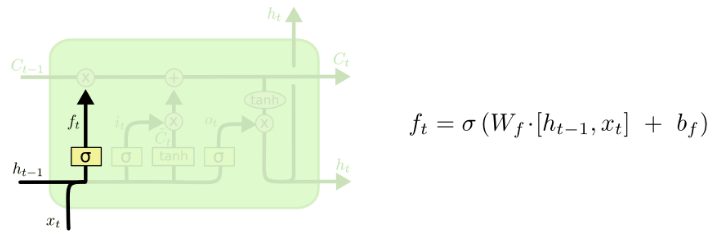
\includegraphics[scale=.5]{image/chapter6/bt1.png}
    \begin{figure}[htp]
    \begin{center}
     
    \end{center}
    \end{figure}
\end{center}
Bước tiếp theo là quyết định xem thông tin mới nào ta sẽ lưu vào trạng thái tế bào. Việc này gồm 2 phần. Đầu tiên là sử dụng một tầng sigmoid được gọi là “tầng cổng vào” (input gate layer) để quyết định giá trị nào ta sẽ cập nhập. Tiếp theo là một tầng $tanh$ tạo ra một véc-tơ cho giá trị mới $\widetilde{C}_{t}$ nhằm thêm vào cho trạng thái. Trong bước tiếp theo, ta sẽ kết hợp 2 giá trị đó lại để tạo ra một cập nhập cho trạng thái.\\
Chẳng hạn với ví dụ mô hình ngôn ngữ của ta, ta sẽ muốn thêm giới tính của nhân vật mới này vào trạng thái tế bào và thay thế giới tính của nhân vật trước đó.
\begin{center}
    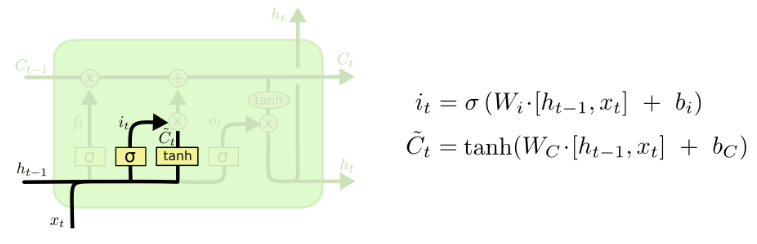
\includegraphics[scale=.5]{image/chapter6/bt2.png}
    \begin{figure}[htp]
    \begin{center}
     
    \end{center}
    \end{figure}
\end{center}
Giờ là lúc cập nhập trạng thái tế bào cũ $C_{t-1}$ thành trạng thái mới $C_{t}$ Ở các bước trước đó đã quyết định những việc cần làm, nên giờ ta chỉ cần thực hiện là xong.\\
Ta sẽ nhân trạng thái cũ với $f_{t}$ để bỏ đi những thông tin ta quyết định quên lúc trước. Sau đó cộng thêm $i_{t} * \widetilde{C}_{t}$. Trạng thái mơi thu được này phụ thuộc vào việc ta quyết định cập nhập mỗi giá trị trạng thái ra sao.\\
Với bài toàn mô hình ngôn ngữ, chính là việc ta bỏ đi thông tin về giới tính của nhân vật cũ, và thêm thông tin về giới tính của nhân vật mới như ta đã quyết định ở các bước trước đó.
\begin{center}
    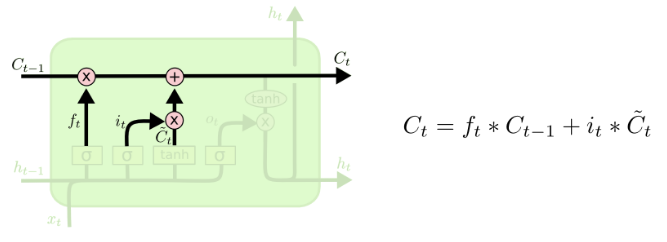
\includegraphics[scale=.5]{image/chapter6/bt3.png}
    \begin{figure}[htp]
    \begin{center}
     
    \end{center}
    \end{figure}
\end{center}
Cuối cùng, ta cần quyết định xem ta muốn đầu ra là gì. Giá trị đầu ra sẽ dựa vào trạng thái tế bào, nhưng sẽ được tiếp tục sàng lọc. Đầu tiên, ta chạy một tầng sigmoid để quyết định phần nào của trạng thái tế bào ta muốn xuất ra. Sau đó, ta đưa nó trạng thái tế bảo qua một hàm tanh để co giá trị nó về khoảng [-1, 1], và nhân nó với đầu ra của cổng sigmoid để được giá trị đầu ra ta mong muốn.\par
Với ví dụ về mô hình ngôn ngữ, chỉ cần xem chủ thể mà ta có thể đưa ra thông tin về một trạng từ đi sau đó. Ví dụ, nếu đầu ra của chủ thể là số ít hoặc số nhiều thì ta có thể biết được dạng của trạng từ đi theo sau nó phải như thế nào.
\begin{center}
    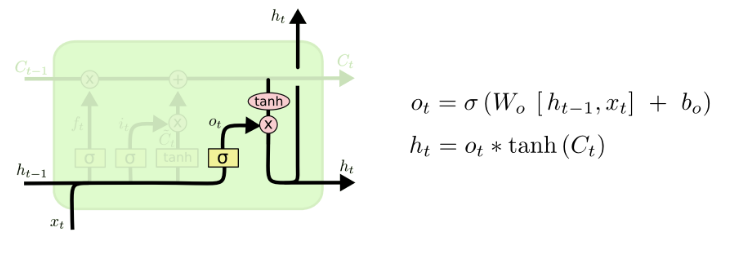
\includegraphics[scale=.5]{image/chapter6/bt4.png}
    \begin{figure}[htp]
    \begin{center}
     
    \end{center}
    \end{figure}
\end{center}


\subsection{Các biến thể của bộ nhớ dài hạn}
Những thứ ta vừa mô tả ở trên là một LSTM khá bình thường. Nhưng không phải tất cả các LTSM đều giống như vậy. Thực tế, các bài báo về LTSM đều sử dụng một phiên bản hơi khác so với mô hình LTSM chuẩn. Sự khác nhau không lớn, nhưng chúng giúp giải quyết phần nào đó trong cấu trúc của LTSM.\\
Một dạng LTSM phổ biến được giới thiệu bởi Gers và Schmidhuber (2000) được thêm các đường kết nối “peephole connections”, làm cho các tầng cổng nhận được giá trị đầu vào là trạng thái tế bào.
\begin{center}
    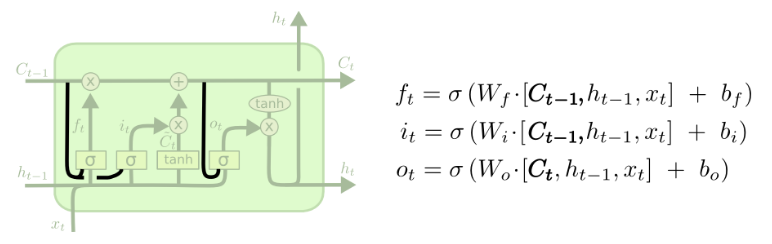
\includegraphics[scale=.5]{image/chapter6/bth1.png}
    \begin{figure}[htp]
    \begin{center}
     
    \end{center}
    \caption{Hình trên mô tả các đường được thêm vào mọi cổng, nhưng cũng có những bài báo chỉ thêm cho một vài cổng mà thôi.}
    \end{figure}
\end{center}
Một biến thể khác là nối 2 cổng loại trừ và đầu vào với nhau. Thay vì phân tách các quyết định thông tin loại trừ và thông tin mới thêm vào, ta sẽ quyết định chúng cùng với nhau luôn. Ta chỉ bỏ đi thông tin khi mà ta thay thế nó bằng thông tin mới đưa vào. Ta chỉ đưa thông tin mới vào khi ta bỏ thông tin cũ nào đó đi.
\begin{center}
    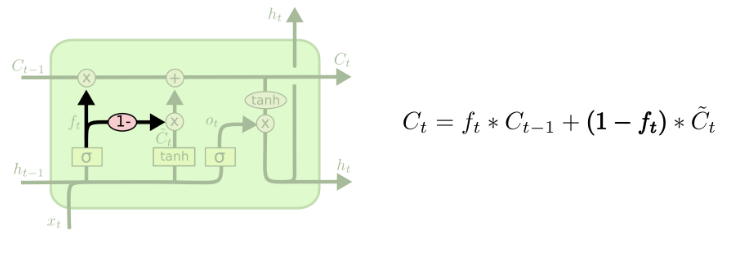
\includegraphics[scale=.5]{image/chapter6/bth2.png}
    \begin{figure}[htp]
    \begin{center}
     
    \end{center}
    \end{figure}
\end{center}
Một biến thể khá thú vị khác của LSTM là Gated Recurrent Unit, hay GRU được giới thiệu bởi Cho, et al. (2014). Nó kết hợp các cổng loại trừ và đầu vào thành một cổng “cổng cập nhập” (update gate). Nó cũng hợp trạng thái tế bào và trạng thái ẩn với nhau tạo ra một thay đổi khác. Kết quả là mô hình của ta sẽ đơn giản hơn mô hình LSTM chuẩn và ngày càng trở nên phổ biến.
\begin{center}
    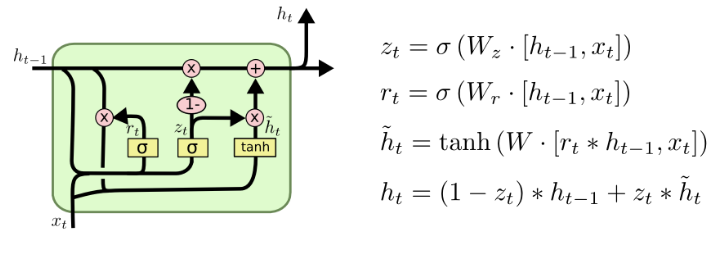
\includegraphics[scale=.5]{image/chapter6/bth3.png}
    \begin{figure}[htp]
    \begin{center}
     
    \end{center}
    \end{figure}
\end{center}
Trên đây chỉ là một vài biến thế được chú ý nhiều nhất thôi, thực tế có rất nhiều các biến thể khác nhau của LSTM như Depth Gated RNNs của Yao, et al. (2015). Cũng có những biến thể mà chiến lực xử lý phụ thuộc xa hoàn toàn khác như Clockwork RNNs của Koutnik, et al. (2014).\\
Nếu bạn muốn tìm hiểu xem biến thể nào là tốt nhất và chúng khác nhau thế nào, thì có thể đọc bài so sánh khá hay này của Greff, et al. (2015). Ngoài ra thì Jozefowicz, et al. (2015) thậm chí còn thử hàng chục nghìn kiến trúc RNN khác nhau và tìm ra một vài mô hình hoạt động tốt hơn cả LSTM ở một số bài toán.


\section{Kết luận}
RNN đặc biệt là LSTM được sử dụng nhiều trong những bài toán về chuỗi dữ liệu: mô hình ngôn ngữ, nhận dạng giọng nói,... Theo bài báo của Shraddha Singh và nhóm nghiên cứu mạng LSTM đem lại kết quả tốt nhất trong số 3 biến thể của RNN trong phân loại ECG-phát hiện đoạn run nhĩ RNN-acc:85.4\%, GRU-acc:82.5\%, LSTM-acc: 88.1\% \cite{ketluanlstm}.

% \chapter{Mô hình phân loại điện tâm đồ }
\newpage

\section{Sơ đồ hệ thống phân loại điện tâm đồ}
\begin{center}
    
\includegraphics[scale=.5]{image/chapter5/system.png}
    \begin{figure}[htp]
    \begin{center}
    \end{center}
    \caption{Sơ đồ hệ thống phân loại điện tâm đồ}
    \end{figure}
\end{center}

\section{Tiền xử lý dữ liệu}
Tín hiệu điện tâm đồ khi được thu nhận từ các thiết bị đo ban đầu có khả năng rất cao bị nhiễu do nhiều yếu tố khác nhau, như nhiễu do ảnh hưởng từ cơ bắp, nhiễu sinh ra từ các thiết bị điện tử, nhiễu từ các điện cực của thiết bị đo điện tâm đồ, power line interference, baseline wander,… Nhiễu có tác động rất lớn đến chất lượng của việc trích xuất đặc trưng và do đó ảnh hưởng đến kết quả bài toán phân loại (việc trích xuất đặc trưng từ tín hiệu điện tâm đồ có thể không chính xác và do đó có thể dẫn đến kết quả phân loại, chẩn đoán bị sai). Vì vậy, tín hiệu điện tâm đồ được thu nhận lúc ban đầu cần phải được khử nhiễu trước khi được thực hiện các bước trích xuất đặc trưng và phân loại. Giải pháp cho việc khử nhiễu đó là lọc nhiễu Butterworth bậc 2 gồm high pass, low pass.
\begin{center}
         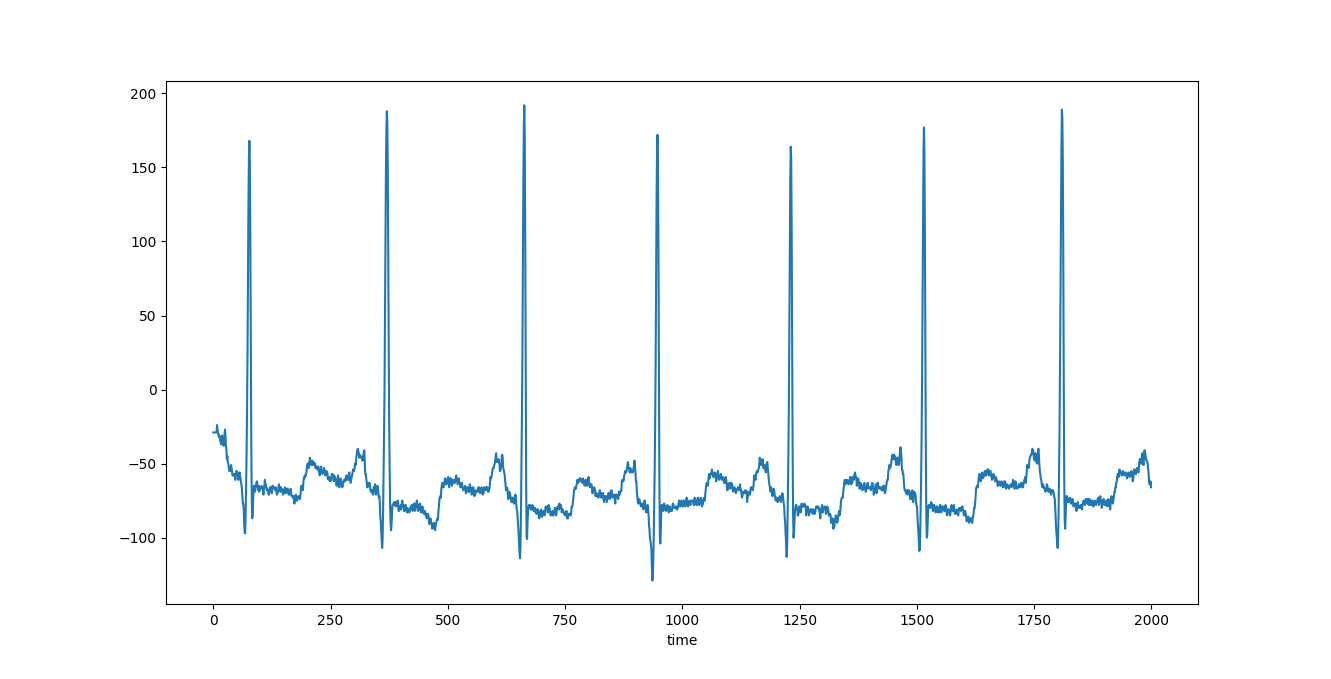
\includegraphics[width=1.\linewidth]{image/chapter5/noise.png}
         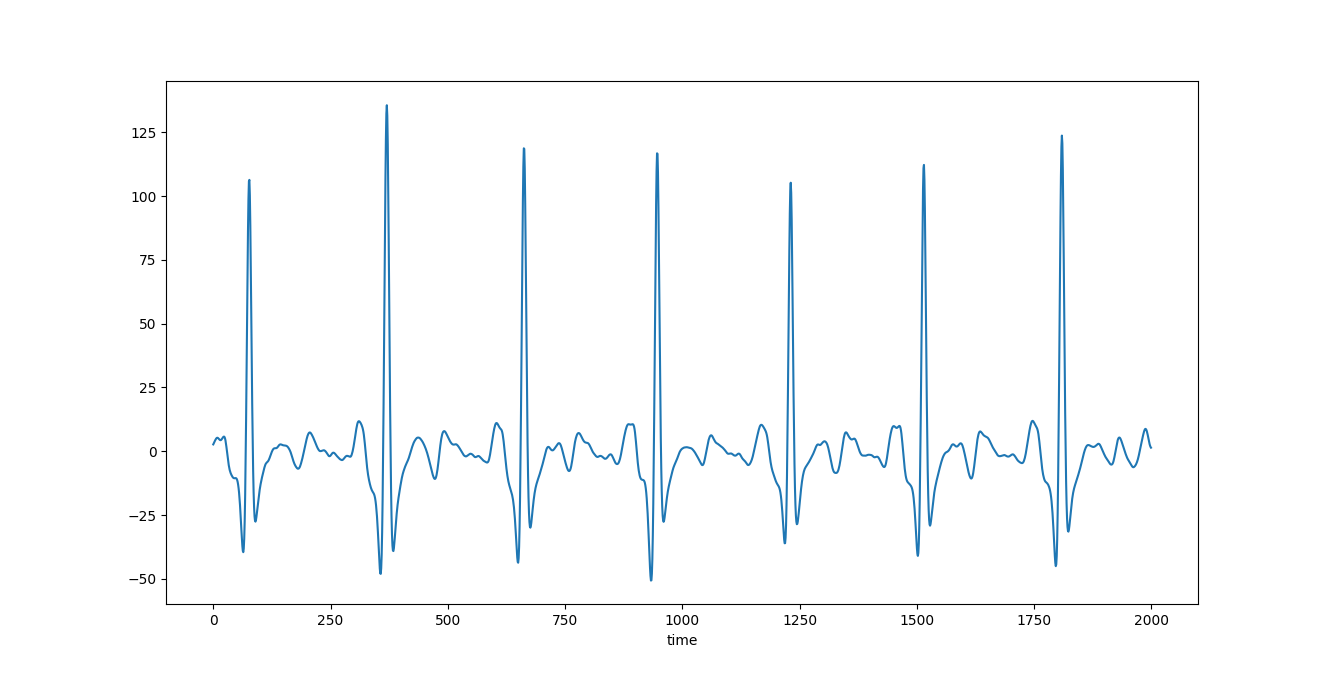
\includegraphics[width=1.\linewidth]{image/chapter5/hlp.png}
    \begin{figure}[!htb]
       \caption{Dữ liệu trước và sau khi lọc nhiễu}
    \end{figure}
\end{center}

\section{Trích xuất đặc trưng}
Dữ liệu sau khi xử lý tiền dữ liệu sẽ được trích xuất đặc trưng bằng kỹ thuật ngưỡng thích ứng kết hợp được đề xuất bới Christov. Những điểm R trong dữ liệu sẽ được đánh nhãn R
\begin{center}
    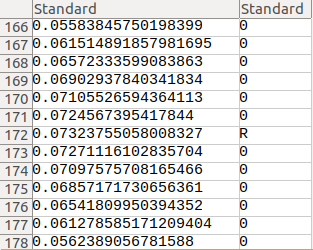
\includegraphics[scale=.5]{image/model/fx_rr.png}
    \begin{figure}[htp]
    \begin{center}
    \end{center}
    \caption{Dữ liệu csv đã được đánh dấu đoạn RR}
    \end{figure}
\end{center}
\begin{center}
    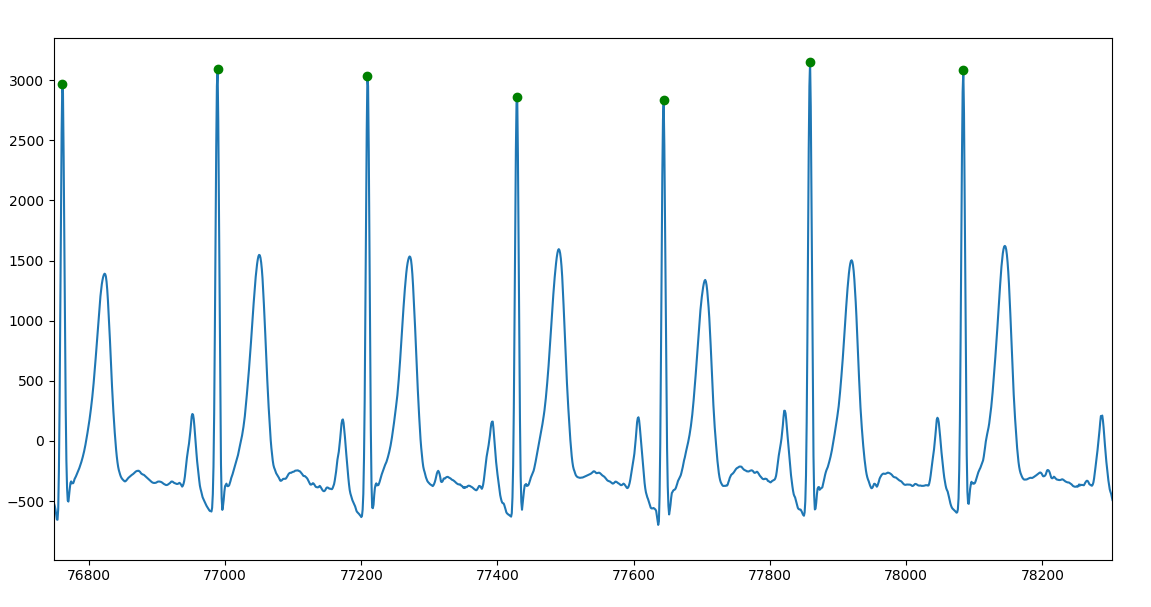
\includegraphics[scale=.4]{image/chapter5/R_detect.png}
    \begin{figure}[htp]
    \begin{center}
    \end{center}
    \caption{Hình ảnh đỉnh R được đánh dấu}
    \end{figure}
\end{center}

\section{Chuẩn hóa đặc trưng độ dài và biên độ khoảng R-R }
Một trong những bước đặc biệt và có ảnh hưởng rất lớn đến chất lượng phân loại tín hiệu điện tâm đồ trong nghiên cứu này là việc chuẩn hóa hình dạng (shape normalization) cho đặc trưng khoảng R-R. Do đặc điểm sinh lý của tim mà các khoảng R-R thường có độ dài khác nhau (nhịp đập của tim thường không bất biến mà sẽ có một sự chênh lệch nhất định). Ở người bình thường, không mắc các bệnh lý về tim mạch, khoảng R-R sẽ dao động trong khoảng 600 – 1200 ms \cite{64} . Sự chênh lệch này tuy không lớn về mặt sinh học nhưng sẽ ảnh hưởng rất lớn đến chất lượng của bài toán phân loại tín hiệu điện tâm đồ. Chỉ một sự thay đổi nhỏ (thậm chí rất nhỏ) về hình dạng khoảng R-R, ví dụ giữa hai đỉnh R có chênh lệch một khoảng nhỏ (ví dụ: 0.01 s), sẽ cho ra một dữ liệu huấn luyện hoàn toàn mới cho bài toán phân loại điện tâm đồ và càng nhiều khoảng R-R có hình dạng dài ngắn khác nhau thì tập dữ liệu huấn luyện được sinh ra sẽ vô cùng lớn. Nếu sự không đồng nhất về mặt hình dạng của các khoảng R-R này không được giải quyết hiệu quả thì việc phân loại những tín hiệu điện tâm đồ mới, không có trong tập dữ liệu huấn luyện, sẽ gặp khó khăn và có thể dẫn đến kết quả phân loại, chẩn đoán không còn chính xác (trường hợp này được gọi là overfit – mô hình phân loại chỉ đáp ứng tốt với dữ liệu huấn luyện mà không còn đáp ứng tốt với dữ liệu kiểm thử hoàn toàn mới). Đó là lý do vì sao các khoảng R-R cần phải được chuẩn hóa về một hình dạng nhất định. Massagram và nhóm nghiên cứu \cite{67}, Bhola và nhóm nghiên cứu đều cho rằng 880 – 900 ms là khoảng thời gian phổ biến nhất của khoảng R-R \cite{68}. Do đó, toàn bộ khoảng R-R trong nghiên cứu này sẽ được chuẩn hóa về khoảng thời gian đồng nhất 900 ms bằng phương pháp nội suy tuyến tính (linear interpolation). Hình dạng của khoảng R-R sau khi đã được chuẩn hóa đồng nhất về cùng một khoảng nhất định sẽ gần như không sai lệch quá nhiều so với khoảng R-R ban đầu. Điều này đồng nghĩa với việc mỗi đoạn R-R sẽ có 324 samples dữ liệu.\\
Dữ liệu sau khi chuẩn hóa về mặt thời gian sẽ được chuẩn hóa tiếp theo chiều cao sóng để đưa về khoảng [0,1] để dể dàng cho việc phân loại.

\section{Phân loại tín hiệu điện tâm đồ}
Mô hìn phân loại tín hiệu điện tâm đồ gồm sự kết hợp giữa mạng LSTM và tâng Fully-connected. Trong đó:
\begin{itemize}
    \item Mạng LSTM ở phần đầu của mô hình có chức năng học những đặc trưng tín hiệu điện tâm đồ có dạng Sequence-to-Sequence (Seq2Seq)
    \item Tầng Fully-Connected ở tầng cuối cùng của mô hình có chức năng phân loại dữ liệu đã được huấn luyện ở mạng LSTM trước đó dựa trên 2 nhãn (label) được cung cấp trước đó là “bình thường” (0) và “bất thường” (1)
\end{itemize}
Các tham số của mô hình phân loại:
\begin{itemize}
    \item Tham số tốc độ học (learning rate) là 0.001, giá trị này ảnh hưởng đến tốc độ hội tụ của quá trình huấn luyện.
    \item Số neuron đầu vào là 128, kích thước thu được khi qua mô hình autoencoder.
    \item Số lượng tầng Fully Connected: 2. Số lượng neuron tầng FC1: 20, số lượng neuron tâng FC2: 20 (có kết hợp kỹ thuật dropout).
    \item Hàm biến đổi: softmax.
    \item Hàm lỗi: Mean Square Error.
    \item Sô lớp phân loại tương ứng với 2 nhãn bình thường (0) và bất thường (1)
    \item Các kỹ thuật tránh overfit: Regularization L2, Dropout, khởi tạo trọng số kiểu Xavier.
    \item Phương pháp tối ưu hóa hàm lỗi: bộ tối ưu SGD.
    \item Số lần tính toán (epoch): 2200.
\end{itemize}

\section{Kết quả, Đánh giá và Trở ngại}
\subsection{Thu thập dữ liệu}
Dữ liệu chủ yếu trong nghiên cứu lần này:
\begin{center}
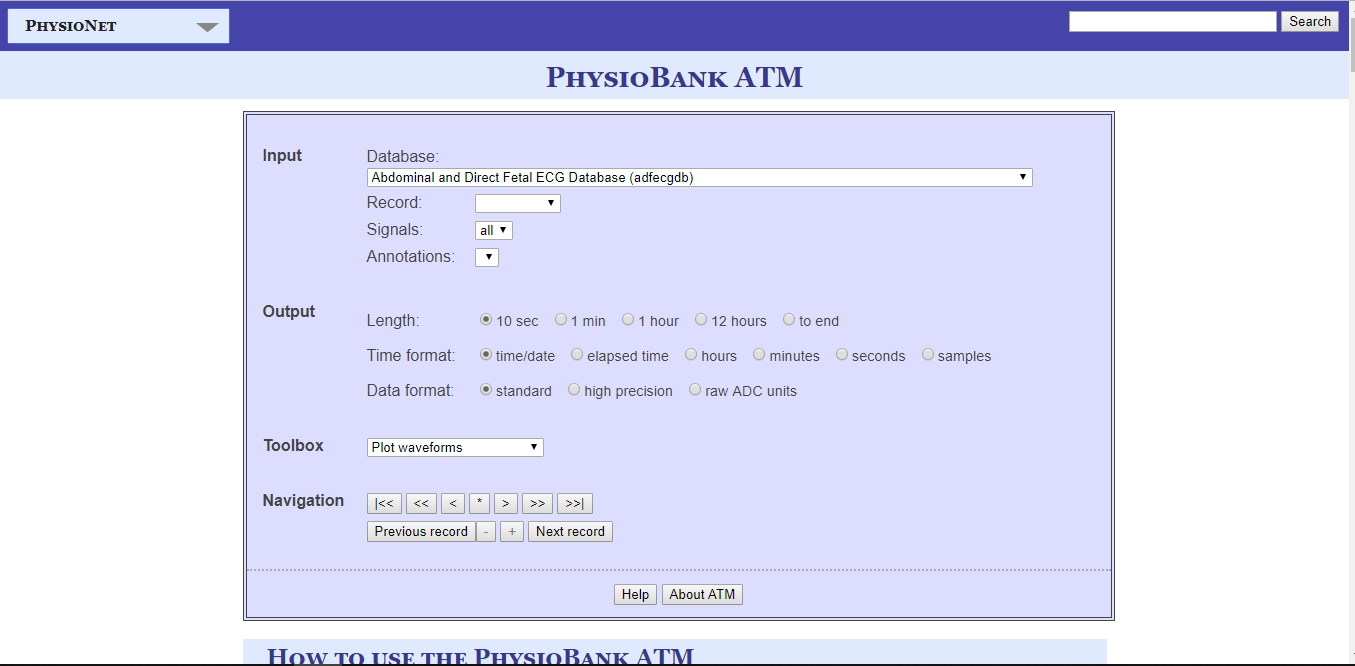
\includegraphics[scale=.3]{image/chapter5/physionet_bank.png}
\begin{figure}[htp]
\begin{center}
\end{center}
\caption{Nguồn thu thập dữ liệu online}
\end{figure}
\end{center}
Bộ dữ liệu được sử dụng: MIT-BIH arrhythmia database.\\
Những đặc điểm của dữ liệu:
\begin{itemize}
    \item Dữ liệu trong thử nghiệm được lấy trên chuyển đạo Lead II trong 2 channel của dữ liệu MIT-BIH vì chuyển đạo này thể hiện rõ ràng nhất đặc điểm của ECG.
    \item Dữ liệu sau khi qua giai đoạn lọc nhiễu và  cắt đoạn RR thu được 98872 (đoạn RR) bao gồm (51765 bình thường và 47107 bất thường)
\end{itemize}
\begin{center}
    \begin{tabular}{|c|c|}
    \hline 
    Tập dữ liệu huấn luyện & Tập dữ liệu kiểm thử \\ 
    \hline 
    79153 & 19719\\ 
    \hline 
    \end{tabular}
\end{center}

\subsection{Kết quả}
Độ chính xác của quá trình phân loại (accuracy): 0.916 và Độ mất mát của quá trình phân loại (loss): 0.052.
\subsection{Đánh giá}
\begin{itemize}
    \item Độ chính xác của mô hình phân loại chưa được cao như những nghiên cứu khác.
\end{itemize}
\subsection{Trở ngoại}
\begin{itemize}
    \item Chỉ mới áp dụng mô hình phân loại trên chuyển đạo Lead II.
    \item Những vấn đề trong việc xử lý dữ liệu, nhiễu...
\end{itemize}


% \chapter{Tổng kết và hướng phát triển}
\newpage

\section{Tổng kết}
Mô hình thực hiện đã dùng các kỹ thuật học sâu: LSTM để thực hiện phân loại và phát hiện bất thường ở ECG .Bên cạnh đó có sử dụng những kỹ thuật signal processing để xử lý tín hiệu điện tâm đồ. Việc phát hiện sớm và điều trị giúp giảm thiểu nguy cơ mắc bệnh tim mạch.

\section{Hướng phát triển}
\begin{itemize}
    \item Mở rộng nguồn dữ liệu, kết hợp nhiều nguồn dữ liệu.
    \item Nghiên cứu phân loại trên những chuyển đạo khác để có những kết quả toàn diện hơn.
    \item Thử nghiệm nhiều mô hình phân loại khác, nghiên cứu và cải tiến để thu được mô hình phân loại tốt nhất
    \item Mở rộng phân loại từng nhóm bệnh cụ thể khi phát hiện có bất thường.
\end{itemize}
% \chapter{Tổng kết}
\section{Tổng kết}
Mô hình thực hiện đã dùng các kỹ thuật học sâu: LSTM để thực hiện phân loại và phát hiện bất thường ở ECG .Bên cạnh đó có sử dụng những kỹ thuật signal processing để xử lý tín hiệu điện tâm đồ. Việc phát hiện sớm và điều trị giúp giảm thiểu nguy cơ mắc bệnh tim mạch.

\section{Hướng phát triển}
\begin{itemize}
    \item Mở rộng nguồn dữ liệu, kết hợp nhiều nguồn dữ liệu.
    \item Nghiên cứu phân loại trên những chuyển đạo khác để có những kết quả toàn diện hơn.
    \item Thử nghiệm nhiều mô hình phân loại khác, nghiên cứu và cải tiến để thu được mô hình phân loại tốt nhất
    \item Mở rộng phân loại từng nhóm bệnh cụ thể khi phát hiện có bất thường.
\end{itemize}
\chapter{Giới thiệu}
\thispagestyle{fancy}
\section{Đặt vấn đề}
Theo ước tính của Tổ chức Y tế thế giới, hàng năm trên thế giới có khoảng 17,5 triệu người tử vong do các bệnh liên quan đến tim mạch và số bệnh nhân tim mạch tích lũy ngày một nhiều. Theo dự báo của Hội Tim mạch Việt Nam, khoảng 20\% dân số nước ta mắc bệnh về tim mạch và tăng huyết áp. Tỷ lệ tăng huyết áp ở những người trẻ từ 25 tuổi đang gia tăng, chiếm 21,5\% tổng số ca mắc bệnh.

% \begin{center}
%     \begin{figure}[htp]
%     \begin{center}
%     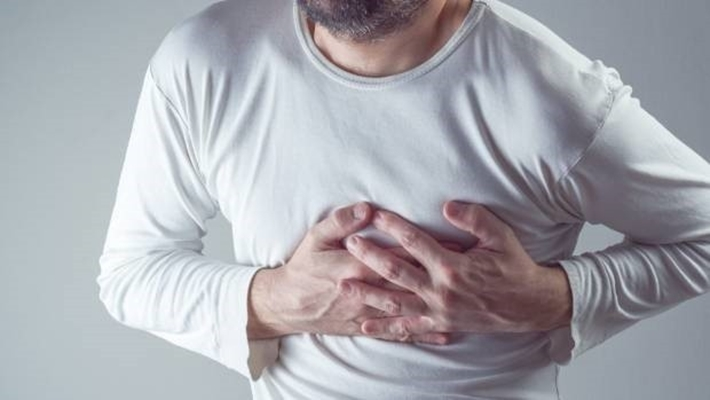
\includegraphics[scale=.4]{image/chapter0/benh-tim-mach-2_0003323_710.jpeg}
%     \end{center}
%     \caption{Số người mắc bệnh tim mạch ngày càng tăng}
%     \end{figure}
% \end{center}
Tuy nhiên, vẫn còn nhiều người thờ ơ, chủ quan và thiếu quan tâm đến sức khoẻ tim mạch của mình. Theo thống kê của Hội tim mạch Việt Nam, vào năm 1980, tỷ lệ mắc bệnh tim mạch ở tuổi 50 trở lên chỉ ở mức 11\%, thì đến năm 2009, tỷ lệ này lên đến 25\% và độ tuổi mắc từ 22 tuổi trở lên\cite{baibao}. Bất thường ở tim mạch có nhiều loại, trong số đó đặc biệt phải nói đến chứng Rối loạn nhịp tim. Rối loạn nhịp tim là một bệnh tim đặc trưng bởi tần số hoặc nhịp tim bất thường: quá nhanh, quá chậm, quá sớm hoặc quá thất thường. Đồng thời bệnh thường phổ biến hơn nhiều với nam giới (70\% các trường hợp), và 30\% bệnh nhân là nữ (theo nghiên cứu thuộc Khoa Y, Trường Cao đẳng Y tế Baroda, Bệnh viện Đa khoa Sir Sayaji, Vadodara, Ấn Độ) \cite{rlnt}.

Rối loạn nhịp tim có thể không có triệu chứng hoặc chỉ gây ra các triệu chứng như: đánh trống ngực, cảm giác đột ngột xuất hiện cơn khó thở - cảm giác khó chịu ở ngực đi kèm,chóng mặt,... Tuy nhiên nhiều trường hợp rối loạn nhịp có thể đe doạ tính mạng của người bệnh và khiến người bệnh phải nhập viện trong tình trạng cấp cứu.

Bệnh có thể gặp ở mọi lứa tuổi và gặp ở cả hai giới, tuy nhiên theo các nghiên cứu thống kê thì bệnh lý rối loạn nhịp gặp nhiều hơn ở các đối tượng sau: tuổi trên 60, người bệnh tăng huyết áp, bệnh động mạch vành, suy tim, bệnh lý van tim, tiền sử phẫu thuật tim mở, ngừng thở khi ngủ, bệnh lý tuyến giáp, đái tháo đường, bệnh phổi mạn tính, lạm dụng rượu hoặc sử dụng chất kích thích, tình trạng nhiễm trùng hoặc bệnh lý nội ngoại khoa nặng...

Việc kiểm tra tim mạch định kì là rất cần thiết theo nhiều khuyến cáo của bộ y tế, tuy nhiên để đo điện tim thì một người phải vào các cơ sở y tế với các thiết bị chuyện dụng, phải thực hiện nhiều kiểm tra, xét nghiệm, cách làm này tốn khá nhiều thời gian và tiền bạc dẫn đến hậu quả là số ca mắc các bệnh tim mạch ngày càng gia tăng và có những biến chứng nguy hiểm.

\section{Mục tiêu}
% \begin{center}
%     \begin{figure}[htp]
%     \begin{center}
%     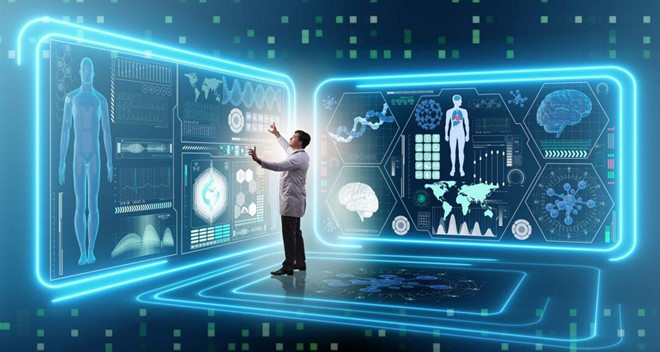
\includegraphics[scale=.4]{image/chapter0/r_sfcc.jpg}
%     \end{center}
%     \caption{Trí tuệ nhân tạo đang phát triển vượt bậc và có nhiều thành tựu trong y khoa}
%     \end{figure}
% \end{center}
Trí tuệ nhân tạo là sự "tư duy" của máy móc, trong đó các thiết bị sẽ bắt chước cách tư duy tự nhiên của con người để giải quyết các vấn đề. Trong cuộc cách mạng công nghiệp 4.0, AI là một trong những yếu tố then chốt. Từ khái niệm tưởng chừng xa xôi, trí tuệ nhân tạo từng bước đi vào đời sống, hiện thực hóa giấc mơ về những loại máy móc có khả năng tư duy như con người. Bên cạnh đó những năm trở lại đây công nghệ internet vạn vật cũng rất phát triển, một vấn đề ta thường nghe nói đến tình trạng quá tải tại các bệnh viện, bệnh nhân không có đủ giường bệnh đề nằm. Sắp tới đây sự ra đời của những chiếc giường thông minh sẽ tạo cảm giác thoải mái tối ưu cho bệnh nhân. Những chiếc giường có thể phát hiện các chuyển động của bệnh nhân và điều chỉnh chiều cao cho phù hợp mà không cần y tá hay can thiệp của con người. Ngoài ra trong thời gian sắp tới sẽ có rất nhiều những thiết bị thông minh ra đời hỗ trợ cho hoạt động khám chữa và điều trị bệnh tại các bệnh viện, phòng khám. Với công nghệ IoT bắt đầu được triển khai ở khắp mọi nơi, sẽ mang lại kết quả tuyệt vời bằng cách giảm chi phí, cải thiện kết quả điều trị, tăng cường trải nghiệm bệnh nhân, giảm lỗi, tăng cường quản lý thuốc và cải thiện quản lý bệnh tật.

Hứa hẹn về ứng dụng của công nghệ trí thông minh nhân tạo (AI) trong ngành y tế là rất lớn, nhiều ứng dụng của trí tuệ nhân tạo vào trong ngành y tế đem lại những thành tựu đáng kể như: robot phẫu thuật có trí thông minh nhân tạo, trợ lý y tá ảo, hỗ trợ đưa ra phác đồ điều trị ung thư,... Vì thế việc áp dụng trí tuệ nhân tạo vào lĩnh vực tim mạch, phát hiện sớm những dấu hiệu bất thường của tim đóng vai trò rất quan trọng giúp giảm nguy cơ mắc các bệnh tim mạch. Trong đó một trong những phương pháp để phát hiện bệnh là đo điện tim. Điện tim là một trong những phương pháp thể hiện rõ nhất những dấu hiệu của tim, điện tim giúp cho bác sĩ phát hiện các bệnh lý như đau ngực, rối loạn nhịp tim, nhồi máu cơ tim, hở van tim, thiếu máu cơ tim,... thông qua việc ghi lại những tín hiệu xung điện qua tim theo một đường truyền dẫn, chúng được hình thành từ các tế bào trong hệ thống cơ tim khi tim hoạt động. Thu thập tín hiệu điện tim từ các thiết bị IoT tiếp qua một hệ thống phân loại để phát hiện sớm các bất thường ở điện tim một cách nhanh chóng và tương đối chính xác sẽ góp phần giám thiểu nguy cơ mắc bệnh tim mạch. Mục tiêu của để tài là sử dụng một hệ thống phân loại sử dụng các kỹ thuật học sâu (Deep Learning) để phát hiện loại bất thường ở điện tim.


\chapter{Tổng quan về điện tâm đồ và một số nghiên cứu liên quan}
\thispagestyle{fancy}

\section{Những khái niêm cơ bản về điện tâm đồ}
\subsection{Định nghĩa}
Điện tâm đồ (ECG) là một đường cong ghi lại các biến thiên của các điện lực do tim phát ra trong khi hoạt động co bóp. Ngoài đo tốc độ và nhịp điệu của tim thì điện tâm đồ còn cung cấp thêm những bằng chứng gián tiếp về lưu lượng máu truyền đến tim. Một xung điện sẽ được tạo ra từ các tế bào trong buồng tim khi tim hoạt động và những tín hiệu khi những xung điện này theo một hệ thống dẫn truyền đi qua tim sẽ được điện tâm đồ ghi lại. Nhờ có điện tâm đồ mà các bác sĩ có thể phát hiện ra được những bệnh lý về tim như loạn nhịp tim, đau thắt ngực,…Thỉnh thoảng, việc tiến hành điện tâm đồ cũng được coi như một xét nghiệm thường quy tại các bệnh viện.
\begin{center}
    \begin{figure}[htp]
    \begin{center}
    %  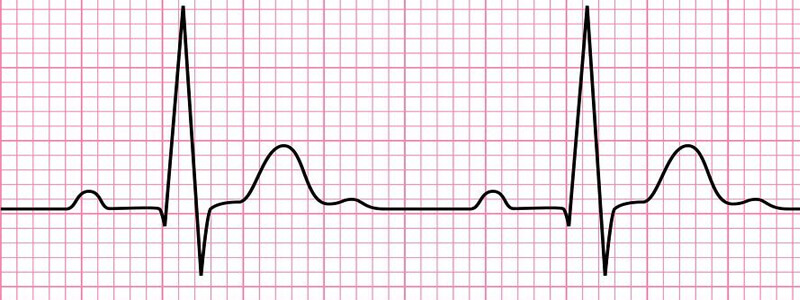
\includegraphics[scale=.]{image/week1/intro.jpg}
     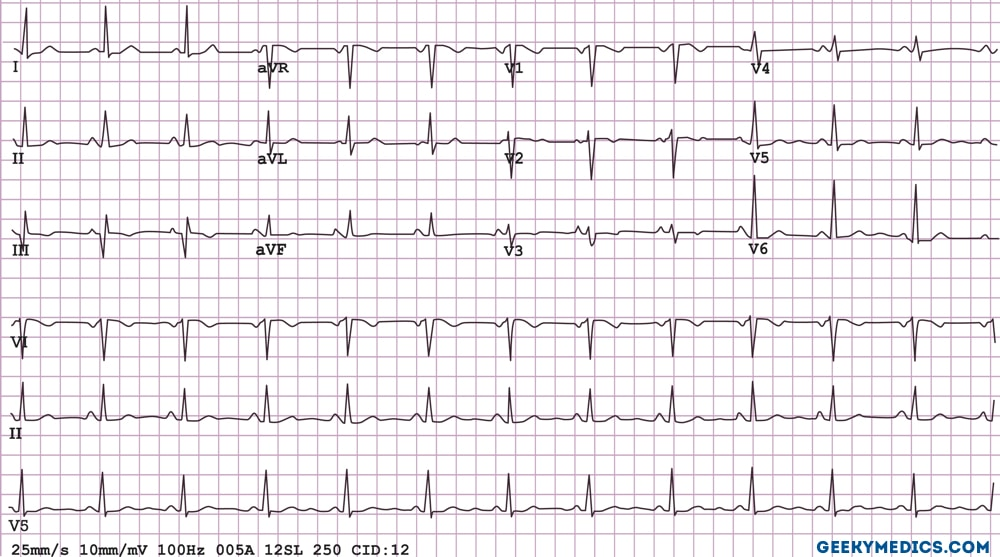
\includegraphics[scale=.35]{image/chapter1/Normal-ECG-SCALED-DOWN-WATERMARK.jpg}
    \end{center}
    \caption{Một đoạn điện tâm đồ }
    \end{figure}
\end{center}

\subsection{Lich sử hình thành điện tâm đồ}
\begin{itemize}
    \item 1887 - Augustus D. Waller (St Mary's Medical School, Luân Đôn) trình bày ECG đầu tiên trên người của Thomas Goswell, một người làm việc trong phòng thử nghiệm.
    \item 1893 - Willem Einthoven giới thiệu từ 'electrocardiogram' tại buổi họp của Hội Y Học Hà Lan (nhưng sau đó ông sửa lại rằng Waller là người đầu tiên dùng chữ này).
    \item 1895 - Einthoven cải tiến dụng cụ và công thức ghi điện, ghi được 5 thay đổi điện trong một nhịp tim, ông ghép chữ cho 5 thay đổi này (P, Q, R, S, T, U).
\end{itemize}

\subsection{Hoạt động điện của cơ tim và sự hình thành điện tâm đồ}
Do sự biến đổi hiệu thế giữa mặt trong và mặt ngoài màng tế bào cơ tim. Sự biến đổi hiệu thế này bắt nguồn từ sự di chuyển của các ion K + , Na + ,... từ ngoài vào trong tế bào và từ trong tế bào ra ngoài khi tế bào cơ tim hoạt động. Lúc này tính thẩm thấu của màng tế bào đối với các ion luôn luôn biến đổi. Do sự chênh lệch nồng độ hai bên màng tạo nên hiệu điện thế giữa hai bên màng (điện thế nghỉ).
\begin{center}
    \begin{figure}[htp]
    \begin{center}
     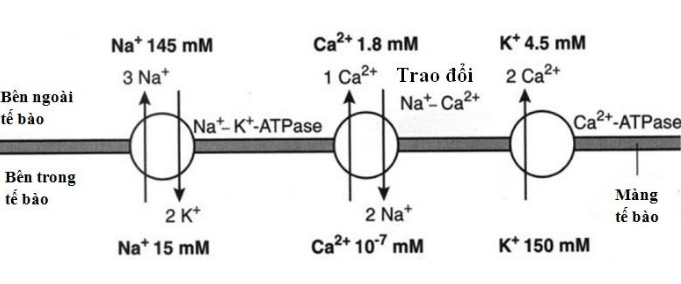
\includegraphics[scale=.4]{image/week1/h21.png}
    \end{center}
    \caption[Sự chênh lệch nồng độ của các ion]{Sự chênh lệch nồng độ của các ion Na, K, Ca trong cơ chế hình thành điện tâm đồ \cite{huongdanDTT}}
    \end{figure}
\end{center}

Tim người có 4 buồng để chứa và bơm máu. Hai phần nhỏ ở phía trên gọi là tâm nhĩ (vì trông giống lỗ tai). Hai phần dưới lớn hơn gọi là tâm thất. Máu theo tĩnh mạch từ cơ thể trở về tâm nhĩ phải, từ phổi trở về tâm nhĩ trái. Tâm nhĩ trái bóp bơm máu vào tâm thất trái, tâm nhĩ phải đưa máu vào tâm thất phải. Sau đó tâm thất phải bóp để bơm máu theo động mạch lên phổi và tâm thất trái bóp để bơm máu xuống cơ thể. Tim có khả năng hoạt động đều đặn và thứ tự như thế là nhờ một hệ thống các tế bào dẫn điện đặc biệt nằm trong cơ tim.

Trong tâm nhĩ bên phải có nút xoang nhĩ (sinoatrial node) gồm các tế bào có khả năng tự tạo xung điện (electric impulse). Xung điện này truyền ra các cơ chung quanh làm co bóp hai tâm nhĩ (tạo nên sóng P trên Điện Tâm đồ). Sau có dòng điện tiếp tục truyền theo 1 chuỗi tế bào đặc biệt tới nút nhĩ thất (atrioventricular node) nằm gần vách liên thất rồi theo chuỗi tế bào sợi Purkinje chạy dọc vách liên thất lan vào các cơ chung quanh (loạt sóng QRS) làm hai thất này co bóp. Sau đó xung điện giảm đi, tâm thất giãn ra (tạo nên sóng T).

\subsection{Các sóng cơ bản và sự hình thành phức bộ sóng}
Một chu kỳ tim biểu hiện trên điện tâm đồ là: sóng P, phức bộ QRS, sóng T, và sóng U (nếu có), hình dạng, thời gian kéo dài của sóng/phức bộ và cả thời gian giữa các thành phần với nhau đều có ý nghĩa đặc biệt quan trọng trong việc chẩn đoán.
\begin{center}
        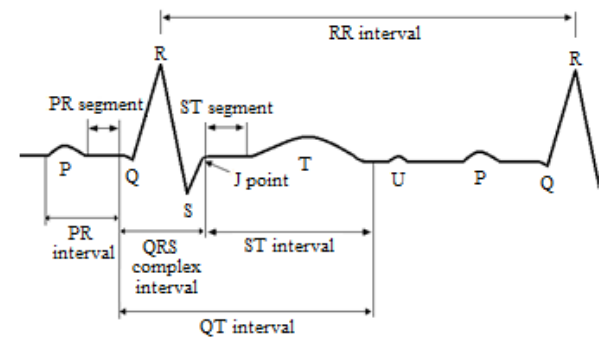
\includegraphics[scale=.4]{image/week1/h32.png}
        \begin{figure}[htp]
        \begin{center}
        \end{center}
        \caption{Tổng hợp những sóng cơ bản}
        \end{figure}
\end{center}

\subsubsection{Các sóng và phức bộ}
\textbf{Sóng P}

Sóng P hình thành do quá trình khử cực tâm nhĩ (cả nhĩ trái và nhĩ phải), bình thường biên độ của sóng P thường dưới 2mm (0.2mmV), và thời gian của sóng P là từ 0.08 đến 0.1 giây, việc tăng biên độ và kéo dài thời gian của sóng gợi ý đến một tình trạng tâm nhĩ lớn (tăng biên độ gợi ý lớn nhĩ phải. thời gian khử cực kéo dài gợi ý đến lớn nhĩ trái).

\textbf{Phức bộ QRS}

Phức bộ QRS thể hiện quá trình khử cực của tâm thất, tùy vào chiều khử cực và vị trí đặt điện cực mà trên giấy ghi sẽ cho thấy các phức bộ khác nhau, ưu thế sóng R hay S, bình thường QRS kéo dài từ 0.06 đến 0.1 giây.
\begin{itemize}
    \item Sóng Q là sóng âm đầu tiên của phức bộ QRS, sóng Q trên bệnh nhân bình thường thường nhỏ và ngắn (hình thành do quá trình khử cực vách liên thất), một sóng Q sâu (biên độ âm lớn) và kéo dài cho thấy một tình trạng hoại tử cơ tim (Trong nhồi máu cơ tim cũ hay nhồi máu cơ tim không có ST chênh lệch).
    \item Sóng R là sóng dương đầu tiên của phức bộ, và sóng âm sau nó là S, đây là hai sóng hình thành do khử cực thất, về bản chất là giống nhau, nếu điện cực đặt ở vị trị chiều khử cực hướng đến thì sóng R sẽ ưu thế, như trong chuyển đạo DII, V5, V6. Sóng R sẽ ưu thế hơn nếu chiều khử cực đi xa vị trí đặt điện cực như V1, V2.
\end{itemize}

\textbf{Sóng T}

Là sóng theo sau phức bộ QRS, thể hiện quá trình tái cực muộn của 2 tâm thất, sóng T có giá trị rất lớn trong việc nhận định một tình trạng cơ tim thiếu máu.
\textbf{Sóng U}
Nguồn gốc sóng U vẫn chưa điện xác định rõ ràng, các giả thuyết đặt ra là:
\begin{itemize}
    \item Tái cực chậm sợi Purkinje.
    \item Tái cực kéo dài giữa cơ tim tế bào M (mid-myocardial cell).
    \item Sau kết quả điện thế của trương lực cơ trong các thành tâm thất.
\end{itemize}
Bình thường không thấy sóng U trên điện tâm đồ, nếu có thì là sóng nhỏ sau sóng T, sóng U đảo ngược hay nhô cao nhọn gặp trong rất nhiều loại bệnh lý tim (bệnh mạch vành, tăng huyết áp, bệnh van tim, tim bẩm sinh, bệnh lý cơ tim, cường giáp, ngộ độc, rối loạn điện giải,...)
\subsubsection{Các đoạn - khoảng}
\textbf{Khoảng PQ}

Là thời gian dẫn truyền từ nhĩ đến thất, bình thường từ 0.12 - 0.2 giây, việc kéo dài thể hiện quá trình chậm dẫn truyền (do bị block), PQ ngắn sẽ gợi ý đến một hội chứng kích thích sớm (Wolf-Parkinson-White)

\textbf{Đoạn ST}

Ý nghĩa là giai đoạn tái cực thất sớm, thời gian của ST thường không quan trọng bằng hình dạng của nó, bình thường ST nằm chênh lệch lên hoặc chênh xuống khỏi đường đẳng điện rất ít. đoạn ST cực kỳ quan trọng trong việc chẩn đoán nhồi máu cơ tim.

ST gọi là chênh lệch nếu cao hơn đường đẳng điện 1mm ở chuyển đạo chi và hơn 2mm ở chuyển đạo trước ngực

ST gọi là chênh xuống khi nằm dưới đường đẳng điện hơn 0.5mm

\textbf{Đoạn QT}

Là thời gian tâm thu điện học của tâm thất, khoảng giá trị bình thường của QT phục thuộc vào tần số tim, QT kéo dài bất thường có liên quan với tăng nguy cơ loạn nhịp thất, đặc biệt là xoắn đỉnh. Gần đây, hội chứng QT ngắn bẩm sinh đã được tìm thấy có liên quan với tăng nguy cơ rung nhĩ và thất kịch phát và đột tử do tim.

\subsection{Các chuyển đạo thông dụng}

\subsubsection{Điện trường tim}
Cơ thể con người là một môi trường dẫn điện; vì thế, dòng điện do tim phát ra được dẫn truyền khắp cơ thể, ra tới da, biến cơ thể thành một điện trường của tim. Nếu ta đặt hai điện cực lên bất cứ hai điểm nào đó có điện thế khác nhau của điện trường đó, ta sẽ thu được một dòng điện thể hiện hiệu thế giữa hai điểm đó và gọi là một chuyển đạo hay đạo trình (lead). Nó hiện ra trên máy ghi bằng một đường cong điện tâm đồ có một hình dạng nào đó tùy theo địa điểm đặt các điện cực. Đường thẳng nối hai địa điểm đặt điện cực trên cơ thể gọi là trục chuyển đạo.

\subsubsection{Chuyển đạo mẩu:}
\begin{center}
    \begin{figure}[htp]
    \begin{center}
    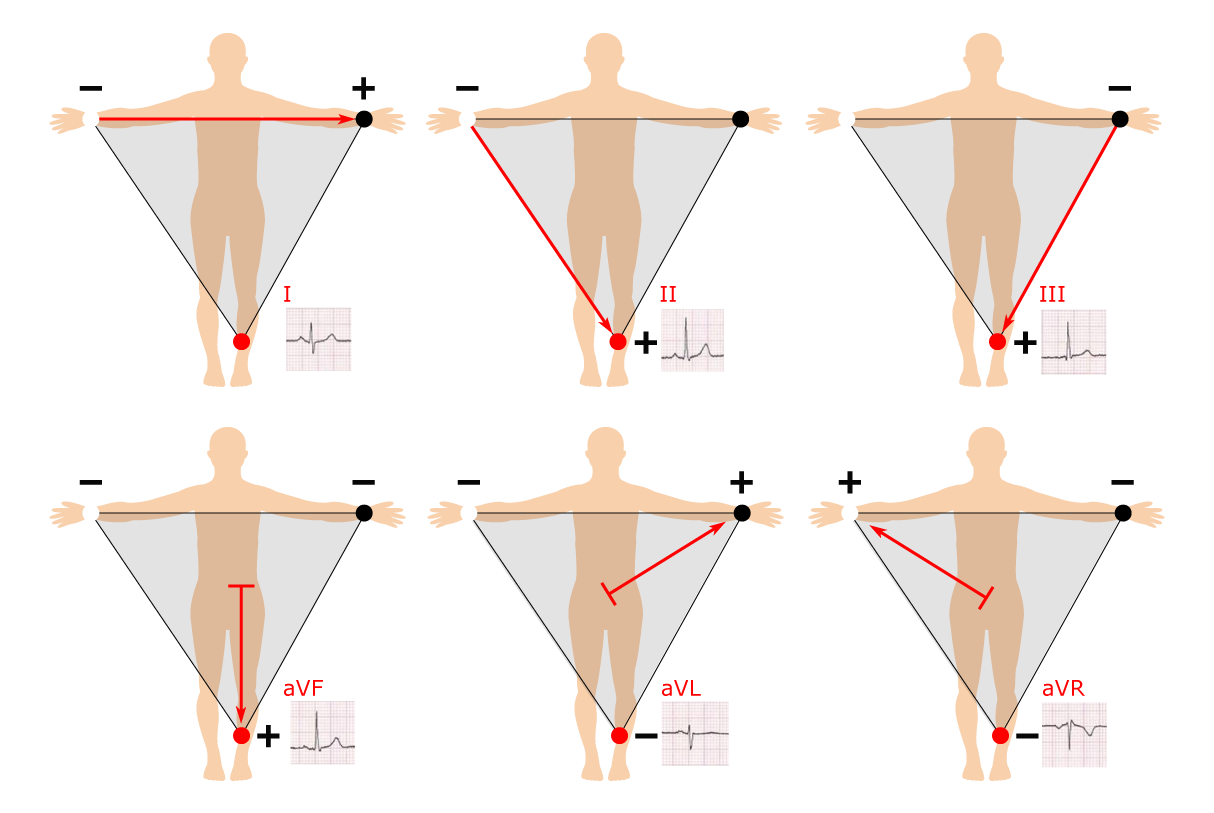
\includegraphics[scale=.2]{image/week1/chuyendaochi.png}
    \end{center}
    \caption[Chuyển đạo chi]{Chuyển đạo chi \cite{chuyendao}}
    \end{figure}
\end{center}
Tất cả 6 chuyển đạo: D1, D2, D3, aVR, aVL, aVF được gọi chung là các chuyển đạo ngoại biên vì đều có điện cực thăm dò đặt ở các chi. Chúng hỗ trợ cho nhau “dò xét” các rối loạn của dòng điện tim thể hiện ở bốn phía xung quanh quả tim trên mặt phẳng chắn (frontal plane).
\begin{center}
    \begin{figure}[htp]
    \begin{center}
    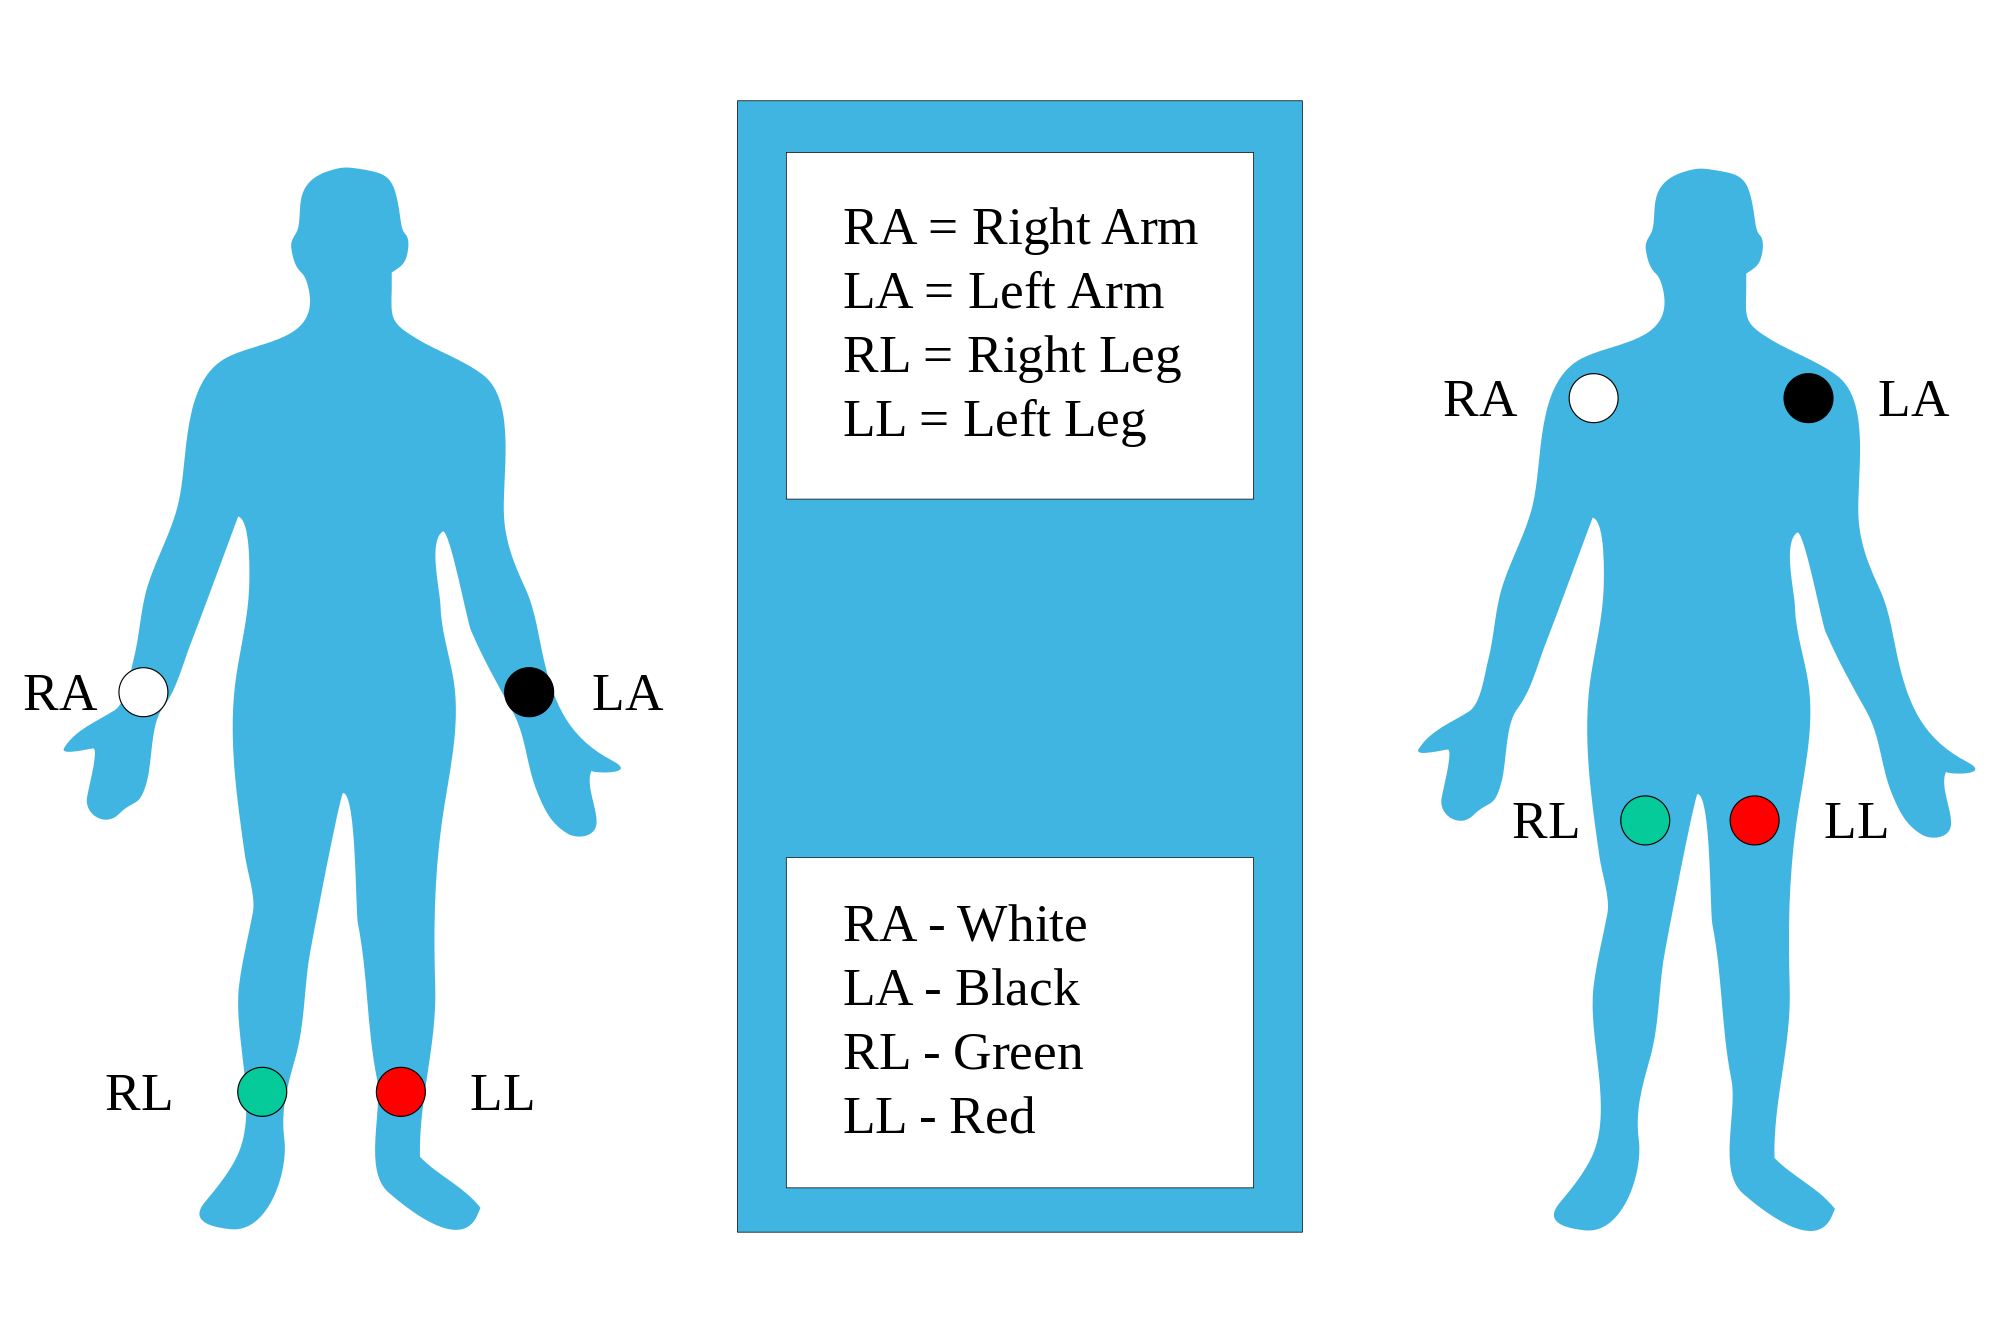
\includegraphics[scale=.12]{image/chapter1/2000px-Limb_leads.png}
    \end{center}
    \caption{Các vị trí đặt điện cực}
    \end{figure}
\end{center}

\subsubsection{Chuyển đạo trước tim:}
\begin{center}
    \begin{figure}[htp]
    \begin{center}
    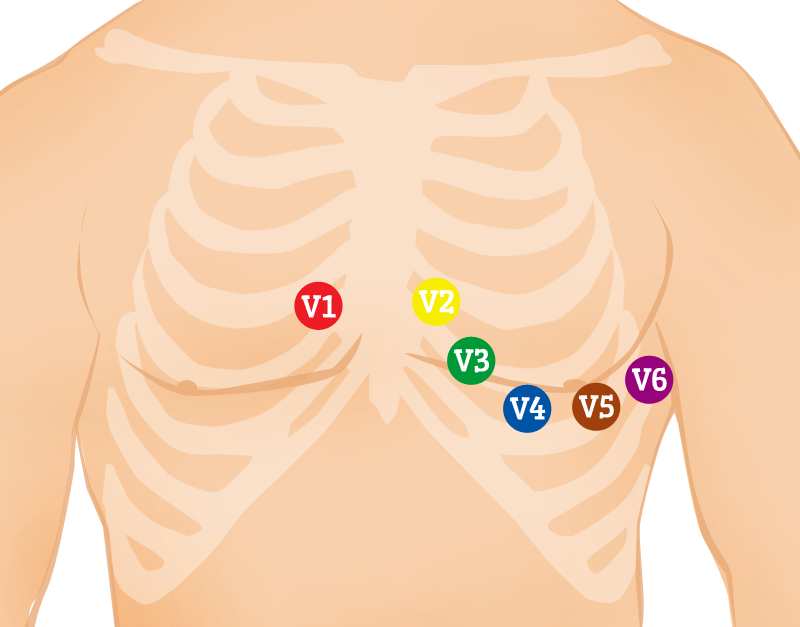
\includegraphics[scale=.25]{image/week1/chuyendaotruocnguc.png}
    \end{center}
    \caption{Chuyển đạo trước tim}
    \end{figure}
\end{center}
Người ta thường ghi đồng loạt cho bệnh nhân 6 chuyển đạo trước tim thông dụng nhất, kí hiệu bằng chữ V (voltage) kèm theo các chỉ số từ 1 đến 6.(V1, V2,…,V6).

\subsubsection{Một số chuyển đạo khác:}
V7, V8, V9(điện cực ở mé trái và sau lồng ngực dùng để thăm dò thất trái), V3R, V4R, V5R, V6R(điện cực ở mé phải lồng ngực dùng để nghiên cứu thất phải hay tim sang phải), chuyển đạo thực quản (Kí hiệu VOE), chuyển đạo trong buồng tim, điện đồ His.

\subsection{Đo điện tâm đồ}
\subsubsection{Đo điện tâm đồ truyền thống}
Định dạng chuẩn của một điện tâm đồ là điện tâm đồ được ghi lại trên một khổ giấy
.Để đánh giá thời gian dài hay ngắn và biên độ cao hay thấp của các làn sóng điện tâm đồ, người ta đinh chuẩn: 
\begin{itemize}
    \item Vận tốc 25mm/s thì mỗi ô 1mm có giá trị 0,04s.
    \item Theo chiều ngang 1 ô lớn tương ứng với 1000ms.
    \item Theo chiều dọc 1 ô lớn tương ứng 500mV.
\end{itemize}
\begin{center}
    \begin{figure}[htp]
    \begin{center}
    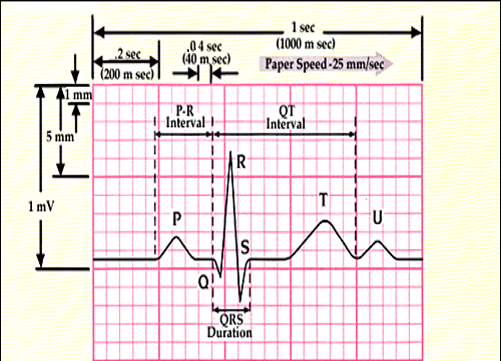
\includegraphics[scale=.6]{image/week1/new_ecg_paper.png}
    \end{center}
    \caption[Hình ảnh một chu kỳ sóng]{Hình ảnh một chu kỳ sóng được đo theo kích thước khổ giấy, bác sĩ căn cứ vào ô trên giấy để phát hiện bất thường ở ECG \cite{ecggiay}}
    \end{figure}
\end{center}
\subsubsection{Đo điện tâm đồ bằng thiết bị di động thông minh (Apple Watch Series 4)}
Tính năng ECG hay còn gọi là đo điện tâm đồ đã chính thức có thể sử dụng trên Apple Watch Series 4 để phát hiện nhịp tim bất thường và chẩn đoán các bệnh tim nghiêm trọng.
\begin{center}
    \begin{figure}[htp]
    \begin{center}
    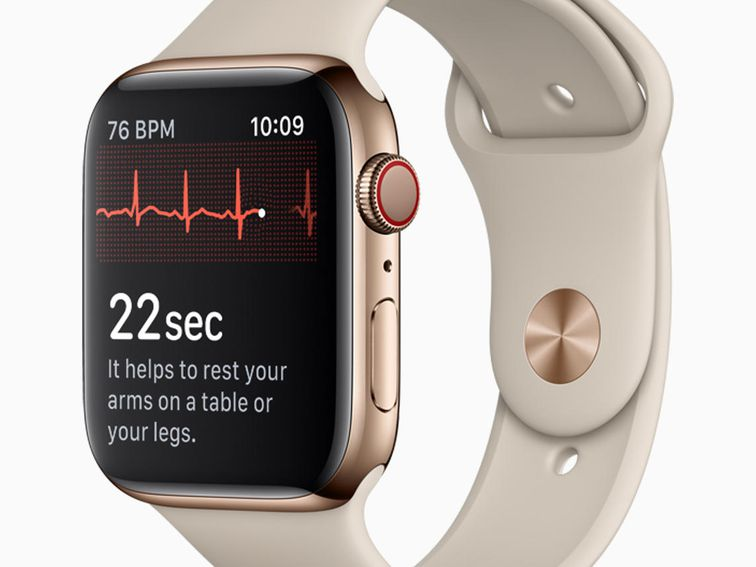
\includegraphics[scale=.3]{image/chapter1/apple-watch-series4-ecg-crown-09122018.jpg}
    \end{center}
    \caption{Apple Watch Series 4}
    \end{figure}
\end{center}
% \section{Đọc một điện tâm đồ}
% \subsection{Những bước phân tích trước khi đọc một điện tâm đồ}
% Điện tâm đồ (ECG) là một đường cong ghi lại các biến thiên của các điện lực do tim phát ra trong khi hoạt động co bóp.\cite{huongdanDTT}

% \begin{enumerate}
%     \item Trước khi đọc điện tâm đồ, phải nắm vững tuổi, giới tính, chẩn đoán lâm sàng của bệnh
%     nhân. Ngoài ra, còn nên biết thêm sơ lược bệnh án, hình ảnh X quang, các kết quả xét nghiệm khác và nhất là hai vấn đề sau đây:
%     \begin{itemize}
%         \item Khổ người bệnh nhân gầy béo, cao thấp ảnh hưởng rất nhiều đến tư thế tìm và biên độ sóng, nó ảnh hưởng nhiều đến chẩn đoán dày thất.
%         \item Có đang dùng thuốc trợ tim hay thuốc chống loạn nhịp dài ngày không? Nhất là digitan và quinidin… vì các thuốc này tác động rất nhiều đến hình dạng điện tâm đồ và dễ làm sai lạc chẩn đoán cơ bản.
%     \end{itemize}
%     \item Kiểm tra kỹ thuật ghi điện tâm đồ, phát hiện ghi sai, ảnh hưởng tạp, milivôn lấy đúng 1cm
%     hay không? Tốc độ ghi bao nhiêu? Nghĩa là các đường kẻ dọc cách nhau bao nhiêu phần trăm
%     giây
%     \item Nhịp tim: bước vào đọc điện tâm đồ trước hết bao giờ cũng phải xem nhịp xoang hay
%     không xoang? Có những rối loạn nhịp tim gì? Đừng bao giờ quên tính tần số tim. Nếu có blốc
%     nhĩ-thất thì phải tính riêng cả tần số nhĩ.
%     \item Trục điện tim với góc alpha, tư thế tim.
%     \item Hình dạng các sóng: đọc đồng thời ở cả 12 chuyển đạo thông dụng:
%     \begin{itemize}
%         \item Sóng P: chiều cao (biên độ), chiều rộng (thời gian), hình dạng (âm, dương, hai pha, móc).
%         \item Khoảng PQ dài bao nhiêu?
%         \item Phức bộ QRS: biên độ và thời gian chung và riêng của sóng Q, hình dạng (móc…).
%         \item Riêng với V1 và V5 thì tìm thêm thời gian xuất hiện nhánh nội điện.
%         \item Đoạn ST có chênh không?
%         \item Sóng T (và sóng U): dạng (dương, âm hay hai pha), biên độ.
%         \item Khoảng QT dài bao nhiêu?
%     \end{itemize}
%     \item Kết luận chẩn đoán: về tổn thương cơ tim và về rối loạn nhịp tim.
% \end{enumerate}


\section{Tìm hiểu một số nghiên cứu liên quan}
\thispagestyle{fancy}
\textbf{Trong nghiên cứu của KS Park và các cộng sự đã sử dụng kỹ thuật SVM phân lớp (Hierarchical Support Vector Machine)} áp dụng phương pháp thống kê đề xuất bậc cao (higher order statistics-HOS) và hàm căn bản Hermite(HBF) để phân loại các nhóm bệnh tim. Theo như nghiên cứu, phức bộ QRS của ECG đóng vai trò rất quan trọng trong nghiên cứu tuy nhiên đặc điểm về hình thái của phức bộ QRS trong lớp N và lớp S khá giống nhau, lớp F và V cũng vậy (các lớp này là label cho việc phân loại, cũng là ký hiệu cho các loại bệnh). Vì vậy, nhóm nghiên cứu đã cân nhắc sử dụng mô hình phân lớp sử dụng SVM để phân loại các lớp có hình thù sóng giống nhau đó. Quá trình phân loại có 2 phase. Ở phase đầu, tiến hành phân loại dữ liệu thành 2 nhóm: nhóm NS và nhóm FV sử dụng HOS,  HBF và những khoảng đặc trưng QRS. Ở phase thứ 2, để phân loại N và S nhóm chỉ sử dụng khoảng RR của dữ liệu. Đối với phân loại V và F ở phase 2, nhóm đã sử dụng toàn bộ đặc trưng đã trích xuất được để thực hiện (bao gồm: khoảng QRS, khoảng RR, trung bình độ dài RR, tỉ số của độ dài RR và trung bình RR). Kết quả cho thấy hệ thống phân loại khá tốt các loại bệnh trong điều kiện phân phối dữ liệu không cân bằng điều mà những hệ thống thông thường chưa đạt được.

\textbf{Trong nghiên cứu của Ozcan và Gurgen đã kết hợp SVM với hướng tiếp cận mờ (fuzzy)} gọi tắt là fuzzy-SVM (FSVM). Phương pháp FSVM định nghĩa mờ input và gán những giá trị thành viên (membership value) cho mỗi input. Ý tưởng của nghiên cứu rất đơn giản đó là sử dụng những cách tiếp cận mờ để định nghĩa trọng số cho input sau đó dùng SVM để phân loại chúng dựa trên những trọng số đã định nghĩa. FSVM giới thiệu khái niệm giá trị thành viên vào SVM dẫn đến việc định nghĩa những hàm thành viên. Một giá trị thành viên cung cấp một bậc (degree) của việc đại diện input cho lớp đó vì vậy một số hàm thành viên được đề xuất trong nghiên cứu: OCW, DTCM, DTOCM, CAR, FCM. Qua nhiều thử nghiệm của nhóm nghiên cứu thì phương pháp FSVM-DTCM đem lại độ chính xác (accuracy) tốt nhất được kiểm nghiệm bằng kỹ thuật 10 fold cross-validation.

\textbf{Andrew Ng và nhóm nghiên cứu đã đề xuất mô hình Convolutional neural network} gồm 34 layers để phân loại chuỗi tín hiệu ECG. Mô hình có thể dự đoán chính xác giữa nhịp xoang (SINUS) và rung nhĩ (AFIB) điều mà nhiều giải thuật khác không làm được. Trước khi cho vào mạng phân loại, dữ liệu sẽ đươc chuẩn hóa để resample. Trước mỗi convolution layer nhóm áp dụng Batch Normalization và một rectified linear activation. Nhóm cũng áp dụng kỹ thuật Dropout giữa các convolution layer và sau các hàm phi tuyến. Cuối cùng là lớp fully connected với hàm kích hoạt softmax gồm 14 lớp output.

\textbf{Saxena và cộng sự trong \cite{classify} đã mô tả một cách tiếp cận đối với các tín hiệu ECG dạng trích xuất tính năng hiệu quả}. Bài báo của họ đề cập đến một phương pháp tổng hợp được phát triển để nén dữ liệu, truy xuất tín hiệu và trích xuất đặc trưng của tín hiệu ECG. Sau khi lấy tín hiệu từ dữ liệu nén, người ta thấy rằng mạng không chỉ nén dữ liệu mà còn cải thiện chất lượng tín hiệu ECG được truy xuất liên quan đến việc loại bỏ nhiễu tần số cao có trong tín hiệu gốc. Với việc triển khai mạng nơ ron nhân tạo (ANN), tỷ lệ nén tăng khi số chu kỳ ECG tăng. Ngoài ra, các tính năng được trích xuất theo tiêu chí biên độ, độ dốc và thời lượng từ tín hiệu thu được khớp với các tính năng của tín hiệu gốc. Kết quả thử nghiệm của họ ở mọi giai đoạn đều đều và ổn định và chứng minh rằng không thể nghi ngờ rằng phương pháp tổng hợp có thể được sử dụng để quản lý dữ liệu hiệu quả và trích xuất tính năng của tín hiệu ECG trong nhiều ứng dụng thời gian thực.

\textbf{Pyakillya và các công sự \cite{cnn1d} Đã tiếp cận theo hướng sử dụng Convolution layer 1D kết hợp với Fully Connected layer} trong phân loại nhịp tim (nhịp xoang bình thường, rối loạn nhịp, các loại nhịp khác và nhiễu loạn). Cụ thể, trong mô hình do Pyakillya đề xuất phần trích xuất đặc trưng áp dụng CNN một cách đặc biệt. Chi tiết kiến trúc mô hình phần loại gồm: 7 convolutional layers với số bộ lọc ngang là 5 and 128 neurons + max-pooling áp dụng dropout cho mỗi layer + GlovalAveragePooling + 3 FCN layers with (256/128/64) neurons + dropout sau mỗi layers + softmax layer cho 4 outputs. Kết quả phân loại thu được cho thấy giải pháp của nhóm nghiên cứu đề xuất có thể phân loại tốt các loại nhịp của ECG trong điều kiện dữ liệu không có cấu trúc rõ ràng và không cân bằng. Ngoài ra giải pháp đề xuất có thể tự trích xuất những thông tin đặc trưng của dữ liệu mà không cần bất kì chuyên gia y tế hay chuyên gia liên quan nào. Tuy nhiên về độ hiệu quả và độ chính xác của giải pháp chưa được cao như những nghiên cứu khác liên quan.


% \section{Tiền xử lý tín hiệu}
% Điện tâm đồ (ECG) là một trong những tín hiệu điện sinh học và nó được sử dụng để ghi lại các hoạt động điện của tim. Tín hiệu của ECG được đặc trưng bởi các sóng PQRS. Loại tín hiệu điện sinh học này chủ yếu được sử dụng trong lâm sàng để xác định các bệnh tim ở Bệnh nhân. Các điện cực bề mặt được sử dụng để đo tín hiệu ECG. Một số nhiễu loạn được tạo ra thông qua điện cực bề mặt này, có thể do các điện cực không được đặt đúng cách trong bệnh nhân. Một số bước để loại bỏ nhiễu về cơ bản là:
% \begin{itemize}
%     \item Kiểm tra da bệnh nhân, tiến hành và chuẩn bị da tốt cho bệnh nhân.
%     \item Kiểm tra gel điện cực.
%     \item Trong thời gian kiểm tra bệnh nhân nên
%     được giữ ấm, không nói và di chuyển.
%     \item Kiểm tra chuyển đạo trước ngực được đặt đúng vị trí hay không. Nếu nó không được đặt đúng cách có nghĩa là nó dẫn đến chẩn đoán sai về
%     nhồi máu cơ tim.
%     \item Kiểm tra kết nối cáp Bệnh nhân với thiết bị ECG
% \end{itemize}
% Đây là những cách được xử lý để loại bỏ nhiểu trong lúc đo tại các trung tâm y tế khi đo điện tâm đồ . Tuy nhiên vẫn còn tồn đọng rất nhiều nhiễu loại như: lệch đường đẳng điện, nhiễu do chuyển động, nhiễu do tiếp xúc các điện cực, nhiễu của thiết bị đo,...Những loại nhiễu loạn này được xử lý bằng nhiều kỹ thuật xử lý tín hiệu. Một số bộ lọc được Rajkumar Patro và nhóm nghiên cứu sử dụng để lọc nhiễu như: Median Filter, Gaussian Filter, Low-pass Butterworth Filter, Window based FIR Filter được thực hiện trên bộ dữ liệu MIT-BIH và đánh giá bằng các độ đo số toàn phương trung bình (MSE) và PSNR. Bên cạnh đó một số kỹ thuật gần đây cũng được áp dụng để lọc nhiễu như: Principle Component Analysis, Neural Network và Wavelet transform, đặc biệt chỉ loại được những tần số cao khỏi sóng và có nhược điểm là băng thông của nó không phải hằng số \cite{130540},\cite{948947}. Karol Antczak đề xuất sử dụng Mạng hồi quy sâu để lọc nhiễu (Deep Recurrent Neural Network) cũng giải quyết được những vấn để trên.

% \section{Trích xuất đặc trưng tín hiệu điện tâm đồ }
% \subsection{Trích xuất đặc trưng}
% Trích xuất đặc trưng tín hiệu điện tim đóng vai trò quan trọng trong chuẩn đoán bệnh tim. Một chu kỳ của nhịp tim gồm các thành phần sóng cơ bản P,Q,R,S,T. Biên độ và chiều dài các thành phần sóng xác định chức năng tim của mỗi con người.\par
% Zhao và cộng sự. [6] đề xuất một phương pháp trích xuất tính năng bằng cách sử dụng wavelet transform và support vector machine. Bài viết trình bày một cách tiếp cận mới để trích xuất đặc trưng để nhận biết nhịp tim đáng tin cậy. Hệ thống phân loại được đề xuất bao gồm ba thành phần bao gồm tiền xử lý dữ liệu, trích xuất đặc trưng và phân loại tín hiệu ECG. Hai phương pháp trích xuất tính năng đa dạng được áp dụng cùng nhau để đạt được vector đặc trưng của dữ liệu ECG. Biến đổi wavelet được sử dụng để trích xuất các hệ số của biến đổi như các tính năng của từng phân đoạn ECG. Đồng thời, mô hình tự phát (AR) cũng được áp dụng để nắm giữ các cấu trúc thời gian của dạng sóng ECG. Sau đó, cuối cùng, support vector machine (SVM) với Gaussian kernel được sử dụng để phân loại nhịp tim ECG khác nhau. Kết quả mô phỏng máy tính được cung cấp để xác định hiệu suất của phương pháp đề xuất đạt độ chính xác tổng thể là 99,68\%.\par
% Một cách tiếp cận mới để trích xuất đặc trưng ECG đã được đưa ra bởi Fidel và các cộng sự trong [7]. Bài báo đề xuất của họ trình bày một thuật toán, dựa trên biến đổi wavelet, để trích xuất tính năng từ tín hiệu điện tâm đồ (ECG) và nhận biết nhịp tim bất thường. Vì các phép biến đổi wavelet có thể được định vị cả trong miền tần số và thời gian. Họ đã phát triển một phương pháp để chọn một sóng mẹ tối ưu từ một tập hợp ngân hàng bộ lọc sóng con trực giao và trực giao bằng phương pháp tương quan tốt nhất với tín hiệu ECG. Bước đầu tiên trong cách tiếp cận của họ là khử nhiễu (loại bỏ nhiễu) tín hiệu ECG bằng ngưỡng mềm hoặc cứng với giới hạn 99,99 tái tạo khả năng và sau đó mỗi chu kỳ PQRST được phân tách thành một vectơ hệ số bằng hàm sóng con tối ưu. Các hệ số, xấp xỉ của mức tỷ lệ cuối cùng và chi tiết của tất cả các cấp, được sử dụng cho ECG được phân tích. Họ đã chia các hệ số của mỗi chu kỳ thành ba phân đoạn có liên quan đến sóng P, phức bộ QRS và sóng T. Tổng các giá trị từ các phân đoạn này đã cung cấp các vectơ đặc trưng của các chu kỳ đơn.\par
% Mahmoodabadi và cộng sự. trong [1] đã mô tả một cách tiếp cận để trích xuất tính năng ECG sử dụng phép biến đổi Daubechies Wavelets. Họ đã phát triển và đánh giá một hệ thống trích xuất điện tâm đồ (ECG) dựa trên biến đổi sóng con đa độ phân giải. Các tín hiệu ECG từ Modified Lead II (MLII) đã được chọn để xử lý. Bộ lọc wavelet với chức năng chia tỷ lệ gần giống với hình dạng của tín hiệu ECG đạt được phát hiện tốt hơn. Bước đầu tiên trong phương pháp của họ là khử nhiễu tín hiệu ECG bằng cách loại bỏ các hệ số sóng con tương đương ở quy mô cao hơn. Sau đó, các phức bộ QRS được phát hiện và mỗi một phức được sử dụng để theo dõi các đỉnh của các sóng riêng lẻ, bao gồm các bộ và sóng của sóng P và T có trong một chu kỳ tim. Kết quả thử nghiệm của họ cho thấy phương pháp tiếp cận được đề xuất của họ cho trích xuất tính năng ECG đạt được độ nhạy (sensitivity) 99,18\% và dự đoán tích cực (positive predictivity) là 98\%.\par
% Saxena và cộng sự trong [10] đã mô tả một cách tiếp cận đối với các tín hiệu ECG dạng trích xuất tính năng hiệu quả. Bài báo của họ đề cập đến một phương pháp tổng hợp được phát triển để nén dữ liệu, truy xuất tín hiệu và trích xuất đặc trưng của tín hiệu ECG. Sau khi lấy tín hiệu từ dữ liệu nén, người ta thấy rằng mạng không chỉ nén dữ liệu mà còn cải thiện chất lượng tín hiệu ECG được truy xuất liên quan đến việc loại bỏ nhiễu tần số cao có trong tín hiệu gốc. Với việc triển khai mạng nơ ron nhân tạo (ANN), tỷ lệ nén tăng khi số chu kỳ ECG tăng. Ngoài ra, các tính năng được trích xuất theo tiêu chí biên độ, độ dốc và thời lượng từ tín hiệu thu được khớp với các tính năng của tín hiệu gốc. Kết quả thử nghiệm của họ ở mọi giai đoạn đều đều và ổn định và chứng minh rằng không thể nghi ngờ rằng phương pháp tổng hợp có thể được sử dụng để quản lý dữ liệu hiệu quả và trích xuất tính năng của tín hiệu ECG trong nhiều ứng dụng thời gian thực.\par
% Một trong những tính chất chung của ECG là đoạn trong R-R (R-R interval) hay nói cách khác là khoản cách từ đỉnh R của chu kỳ sóng này đến đỉnh R của chu kỳ sóng kia. Ngoại trừ những bệnh nhân sử dụng máy tạo nhịp tim, những thay đổi về độ rộng của đoạn R-R có liên quan đến hình thái đường cong của nhịp tim, và những biến đổi này thường là dấu hiệu của việc rối loạn nhịp tim. Vì vậy, các đặc trưng trong khoảng RR có khả năng lớn để phân biệt các loại nhịp tim và một số tác giả áp dụng các phương pháp của mình chỉ dựa vào các đặc trưng khoảng RR [67-69].\par
% Lin và Yang [41] đã chỉ ra rằng việc sử dụng khoảng R-R chuẩn hóa giúp cải thiện đáng kể kết quả phân loại. Chỉ các khoảng RR chuẩn hóa được sử dụng trong nghiên cứu đó và kết quả có thể so sánh với các phương pháp tiên tiến ngay cả trong mô hình liên bệnh nhân. Doquire và các đồng nghiệp [71] đã xác nhận hiệu quả của các khoảng RR được chuẩn hóa bằng các kỹ thuật lựa chọn đặc trưng.\par
% Các đặc trưng từ miền thời gian/tần số của các đặc trưng trong khoảng R-R được sử dụng trong các nghiên cứu gần đây đem lại sự chính xác cao nhất cho mô hình phân loại. Nhằm mục đích giảm kích thước của vectơ đặc trưng,...các kỹ thuật khác nhau đã được áp dụng trực tiếp trên các mẫu (samples) đại diện cho nhịp tim (trong vùng lân cận của đỉnh R) như phân tích thành phần chính (PCA) [75-77] hoặc phân tích thành phần độc lập ( ICA) [78-80], trong đó các hệ số mới được trích xuất để biểu thị nhịp tim. Chawla [81] trình bày một nghiên cứu so sánh giữa việc sử dụng PCA và ICA để giảm nhiễu và tạo tín hiệu của tín hiệu ECG và cho thấy PCA là một kỹ thuật tốt hơn để giảm nhiễu, trong khi ICA là phương pháp tốt hơn để trích xuất các tính năng. Kỹ thuật ICA cho phép tách riêng các nguồn riêng biệt khỏi tín hiệu trộn. Hơn nữa, người ta đã chứng minh rằng sự kết hợp của hai kỹ thuật này, tức là PCA để giảm nhiễu và ICA để trích xuất tính năng, có thể mang lại lợi thế lớn hơn khi so sánh chỉ sử dụng một trong số chúng.

% \section{Phân loại điện tim}
% Khi tập hợp các đặc trưng đã được xác định từ nhịp tim, ta có thể áp dụng mô hình phân loại bằng những kĩ thuật học máy, học sâu. Có 4 kỹ thuật phổ biến được sử dụng trong các nghiên cứu về phân loại điện tim từ trước đến nay.\par
% Support Vector Machine (SVM) là một trong những phân loại phổ biến nhất được tìm thấy trong tài liệu cho các phương pháp phân loại rối loạn nhịp tim dựa trên ECG. Park và cộng sự [7] đã sử dụng SVM trong cấu hình phân cấp giả để giải quyết sự mất cân bằng của cơ sở dữ liệu MIT-BIH và báo cáo các giá trị đầy hứa hẹn. de Lannoy và cộng sự [32] đã cố gắng khắc phục sự mất cân bằng của cơ sở dữ liệu MIT-BIH với SVM. Các cách tiếp cận khác nhau với các biến thể SVM đã được đề xuất, chẳng hạn như kết hợp lý thuyết mờ để tinh chỉnh phân loại SVM [117], kết hợp với một nhóm các phân loại [42], thuật toán di truyền kết hợp với SVM mờ hạn chế [118] và SVM bình phương nhỏ nhất [104]. Huang et al đã sử dụng SVM theo cách phân cấp với chiến lược bỏ phiếu tối đa và báo cáo những cải tiến đáng kể. Moavenian và Khorrami [119] đã đề xuất sử dụng hàm kernel mới để thu thập dữ liệu từ SVM và đã được sử dụng cùng một phương pháp để so sánh các kết quả thu được từ một mạng lưới thần kinh nhân tạo đa lớp (MLP-ANN). Mặc dù SVM hiệu quả hơn trong thời gian thực hiện, cả trong huấn luyện và kiểm thử , MLP hoạt động tốt hơn về accuracy, sensitivity, positive prediction (+ P) và false positive rate (FPR). Vì SVM không hoạt động tốt đối với sự mất cân bằng trong các lớp dữ liệu huấn luyện, các kỹ thuật cân bằng cơ sở dữ liệu cho giai đoạn huấn luyện, ít được khám phá cho vấn đề này, có thể được nghiên cứu trong nghiên cứu trong tương lai để cải thiện SVM.\par
% Kiến trúc mạng neural nhân tạo (ANN) được sử dụng nhiều trong phân loại loạn nhịp là Multilayer Perceptrons (MLP) and Probabilistic Neural Networks (PNN). Theo Yu và Chen [101], các mô hình được xây dựng bằng PNN có tính toán mạnh mẽ và hiệu quả hơn so với MLP truyền thống. Nhiều cách tiếp cận dựa trên ANN cũng được đề xuất. Mar và cộng sự [34] đã so sánh MLP với Phân biệt tuyến tính (Linear Discriminant) và thấy rằng MLP vượt trội hơn đáng kể. Theo Osowski và các đồng nghiệp, việc kết hợp các mô hình phân loại không những giảm thiểu lỗi của mạng neural mà còn giảm tỉ lệ false negatives (NP).\par
% Những kỹ thuật học không giám sát như KNN cũng được đề xuất, tuy nhiên không được sử dụng nhiều trong phân loại điện tim, vì hiệu quả của chúng được liên kết mật thiết với kiến thức trước đó dẫn đến chi phí tính toán cao trong giai đoạn thử nghiệm. Mishra và Raghav [95] đã sử dụng một bộ phân loại dựa trên kNN và báo cáo kết quả đầy hứa hẹn, tuy nhiên chi phí tính toán không được đề cập.\par
% Hidden markov model (HMM) được sử dụng nhiều trong tính hiệu âm thanh và văn bản để phân tích và nhận diện. Coast và các cộng sự [132] dùng HMM cho việc  phân tích và phân loại điện tim.\par
% Phương pháp sử dụng cây quyết định cũng là một trong những phương pháp được đề xuất trong lĩnh vực này. Tuy nhiên, phương pháp này không hiệu quả cho tập dữ liệu số thực liên tục và vector đặc trưng có số chiều lớn. Vì vậy Mert và các cộng sự [147] kết hợp kỹ thuật Bagging và Cây quyết định tạm gọi là Bagged Decision Tree đã đem lại kết quả khá khả quan.\par
% Một số nghiên cứu khác: Trong nghiên cứu \cite{11}, phân loại điện tim dựa trên Neural Network và Fuzzy. Trong nghiên cứu \cite{12}, sự khác nhau giữa sóng bình thường được phân loại bằng cách sử dụng (Linear Discriminant Analysis) LDA and Artificial Neural Networks (ANN). Một số nghiên cứu cho thấy MLP (Multilayer Perception) được dùng trong ANN tốt hơn phân loại LDA. MLP trong ANN được sử dụng để tìm bình thường và bất thường ở ở nhịp tim. Principal component analysis (PCA) và một số cấu trúc neural network được sử dụng và phân loại điện tim. Kết quả của việc này là để tìm ra mô hình neural network phù hợp nhất cho từng loại loạn nhịp khác nhau. Trong nghiên cứu \cite{13}, để thu giảm chiều dữ liệu bằng PCA. Bài báo này đã kết hợp các giải thuật phân cụm giữa FCA và PCA neural networ, và đã chứng minh sự kết hợp này tốt hơn là sử dụng riêng lẻ. Sự so sánh giữa các giải thuật xác định loạn nhịp tim được sử dụng trong nghiên cứu \cite{14}. Trong đó KNN cũng được sử dụng để xác định QRS. Trong nghiên cứu \cite{rnn}, Shraddha Singh và nhóm nghiên cứu đã phân loại ECG bằng mạng Neuron hồi quy và các biến thể để phân loại điện tim.

\chapter{Kiến thức nền tảng}
\thispagestyle{fancy}

\section{Kỹ thuật lọc nhiễu Butterworth}
Bộ lọc Butterworth là một loại bộ lọc xử lý tín hiệu được thiết kế để có đáp ứng tần số càng phẳng càng tốt trong băng thông. Nó cũng được gọi là một bộ lọc cường độ phẳng tối đa. Nó được mô tả lần đầu tiên vào năm 1930 bởi kỹ sư và nhà vật lý người Anh Stephen Butterworth trong bài báo của ông có tựa đề "Về lý thuyết của bộ khuếch đại bộ lọc".

Giống như tất cả các bộ lọc, nguyên mẫu điển hình là bộ lọc thông thấp, có thể được sửa đổi thành bộ lọc thông cao hoặc được đặt nối tiếp với các bộ lọc khác để tạo các bộ lọc thông dải và dừng băng tần và các phiên bản thứ tự cao hơn của các bộ lọc này.

\begin{center}
    \begin{figure}[htp]
    \begin{center}
    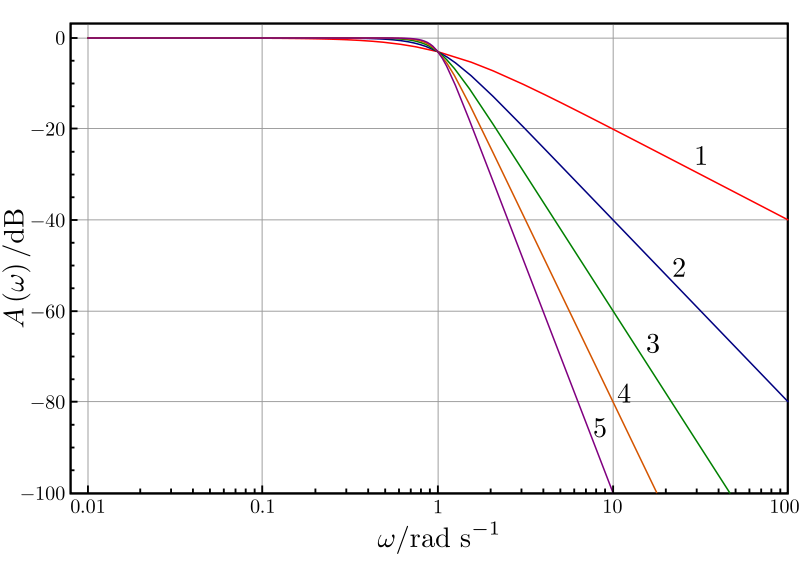
\includegraphics[scale=.4]{image/chapter4/800px-Butterworth_Filter_Orders.png}
    \end{center}
    \caption[Mức đạt được các bộ lọc thông thấp]{Hình vẽ mức đạt được các bộ lọc thông thấp của Butterworth từ 1 đến 5, với tần suất cắt $\omega_0 = 1$. Lưu ý rằng độ dốc là $20n$dB/10 trong đó n là thứ tự bộ lọc.}
    \end{figure}
\end{center}
$G(\omega)$ của bộ lọc thông thấp Butterworth theo thứ tự được đưa ra theo hàm biến đổi $H(s)$ như sau:\\

$G^2(\omega) = \vert{H(j\omega)}^2 = \frac{G_0^2}{1+(\frac{j\omega}{\omega_c})^2}$
Trong đó:
\begin{center}
    \begin{itemize}
        \item $n$: thứ tự bộ lọc 
        \item $\omega_c$: tần số cắt (xấp xỉ -3dB)
        \item $G_0$: Mức tăng DC (mức ở tần số 0)
    \end{itemize}
\end{center}
Có thể thấy rằng khi $n$ tiến đến vô cùng, Đồ thị sẽ trở thành hàm hình chữ nhật và tần số bên dưới $\omega_c$ sẽ được thông qua với mức $G_0$, trong khi tần số ở trên $\omega_c$ sẽ được bỏ đi. Với những giá trị $n$ nhỏ hơn điểm cắt sẽ kém sắt nhọn hơn.

Chúng ta muốn xác định hàm biến đổi $H(s)$ khi $s = \sigma + j\omega$ (từ biến đổi Laplace). Bởi vì $\vert H(s) \vert^2 = H(s)\overline{H(s)}$ và như một tính chất chung của biến đổi Laplace
at $s = j\omega, H(-j\omega) = \overline{H(-j\omega)}$ nếu chúng ta chọn $H(s)$ như sau:
\begin{equation}
H(s)H(-s)=\frac{G_0^2}{1+(\frac{-s^2}{\omega_c^2})^2}
\label{eq:Hs}
\end{equation}

Khi đó, với $s = j\omega$, chúng ta có tần số phản hồi của lọc Butterworth.

Các cực $n$ của biểu thức này xảy ra trên một vòng tròn bán kính $\omega_c$ tại mỗi điểm cách đều nhau và đối xứng xung quanh trục thực âm. Do đó hàm biến đổi $H(s)$ được chọn sao cho chỉ chứa nửa trục thực của $s$. Cực thứ K (k = 1,2,3...,n) được xác định bởi:\\

$-\frac{s_k^2}{\omega_c^2} = (-1)^\frac{1}{n} = e^\frac{j(2k-1)\pi}{n}$ \\

Và vì vậy: \\

$s_k = \omega_c e^\frac{j(2k+n-1)\pi}{2n}$ \\

Hàm biến đổi (hay Hàm hệ thống) có thể được ghi lại trên cùng biểu thức như sau: \\

$H(s) = \frac{G_0}{\prod_{n}{k=1}(s - s_k)/\omega_c}$ \\

Trong đó $\prod$ là phép nhân các toán hạn. Mẫu số là một đa thức Butterworth trong $s$.

\section{Kỹ thuật ngưỡng kích ứng thích hợp}

\section{Mạng Neural Hồi quy (RNN)}
\subsection{Giới thiệu}
Con người không bắt đầu suy nghĩ của họ từ đầu tại tất cả các thời điểm. Cũng như bạn đang đọc bài viết này, bạn hiểu mỗi chữ ở đây dựa vào từ bạn đã hiểu các chữ trước đó chứ không phải là đọc tới đâu ném hết đi tới đó, rồi lại bắt đầu suy nghĩ lại từ đầu tới chữ bạn đang đọc. Tức là tư duy đã có một bộ nhớ để lưu lại những gì diễn ra trước đó.

Tuy nhiên các mô hình mạng nơ-ron truyền thống thì không thể làm được việc đó, đó có thể coi là một khuyết điểm chính của mạng nơ-ron truyền thống. Ví dụ, bạn muốn phân loại các bối cảnh xảy ra ở tất cả các thời điểm trong một bộ phim, thì đúng là không rõ làm thế nào để có thể hiểu được một tình huống trong phim mà lại phụ thuộc vào các tình huống trước đó nếu sử dụng các mạng nơ-ron truyền thống.

Mạng nơ-ron hồi quy (Recurrent Neural Network) sinh ra để giải quyết vấn đề đó. Mạng này chứa các vòng lặp bên trong cho phép thông tin có thể lưu lại được. \cite{rnn-basic}
\begin{center}
    \includegraphics[scale=.5]{image/chapter6/RNN-node.png}
    \begin{figure}[htp]
    \begin{center}
    \end{center}
    \caption{Mạng Neuron hồi quy cấu trúc rút gọn}
    \end{figure}
\end{center}
Một đoạn của mạng nơ-ron hồi quy A với đầu vào là $x_{n}$ và đầu ra là $h_{t}$. Một vòng lặp cho phép thông tin có thể được truyền từ bước này qua bước này qua bước khác của mạng nơ-ron.
Một mạng nơ-ron hồi quy có thể được coi là nhiều bản sao chép của cùng một mạng, trong đó mỗi đầu ra của mạng này là đầu vào của một mạng sao chép khác.

\begin{center}
    \includegraphics[scale=.5]{image/chapter6/RNN-ab.png}
    \begin{figure}[htp]
    \begin{center}
    \end{center}
    \caption{Cấu trúc mạng neuron hồi quy duỗi}
    \end{figure}
\end{center}
Chuỗi lặp lại các mạng này chính là phân giải của mạng nơ-ron hồi quy, các vòng lặp khiến chúng tạo thành một chuỗi danh sách các mạng sao chép nhau.

Một cách chi tiết hơn. 
\begin{center}
    \includegraphics[scale=.4]{image/chapter6/rnn-detail.png}
    \begin{figure}[htp]
    \begin{center}
     
    \end{center}
    \caption{Chi tiết mạng RNN}
    \end{figure}
\end{center}
\begin{itemize}
    \item $x_{t}$ là đầu vào tại bước t.
    \item $s_{t}$ là trạng thái ẩn tại bước t. Nó chính là bộ nhớ của mạng. $s_{t}$ được tính toán dựa trên cả các trạng thái ẩn phía trước và đầu vào tại bước đó: $s_{t} = f(Ux_{t}+Ws_{t-1})$. Hàm $f$ thường là một hàm phi tuyến như tang hyperbolic (tanh) hay Relu. Để làm phép toán cho phần tử ẩn đầu tiên ta cần khởi tạo thêm $s_{-1}$, thường giá trị khởi tạo được gắn bằng 0.
    \item $o_{t}$ là đầu ra tại bước t. Ví dụ, ta muốn dự đoán từ tiếp theo có thể xuất hiện trong câu thì $o_{t}$ chính là một vec-tơ xác xuất các từ trong danh sách từ vựng của ta: $o_{t} = softmax(Vs_{t})$. 
\end{itemize}


\subsection{Một số ứng dụng của RNN}
\begin{itemize}
    \item Nhận dạng giọng nói: Đưa vào một chuỗi các tín hiệu âm thanh, ta có thể dự đoán được chuỗi các đoạn ngữ âm đi kèm với xác xuất của chúng.
    \item Mô tả hình ảnh: Cùng với ConvNet, RNN được sử dụng để tự động tạo mô tả cho các ảnh chưa được gán nhãn. Sự kết hợp này đã đưa ra được các kết quả khá kinh ngạc. Ví dụ như các ảnh dưới đây, các mô tả sinh ra có mức độ chính xác và độ tường tận khá cao.
    \begin{center}
    \includegraphics[scale=.4]{image/chapter6/RNN-application.png}
    \begin{figure}[htp]
    \begin{center}
    \end{center}
    \caption{Ứng dụng của RNN trong phân loại ảnh}
    \end{figure}
    \end{center}
\end{itemize}


\subsection{RNN mở rộng}
\begin{itemize}
    \item RNN 2 chiều: Ở mô hình RNN 2 chiều (Bidirectional RNN), đầu ra tại bước t không những phụ thuộc vào các phần tử phía trước mà còn phụ thuộc cả vào các phần tử phía sau. Ví dụ, để dự đoán từ còn thiếu trong câu, thì việc xem xét cả phần trước và phần sau của câu là cần thiết. Vì vậy, ta có thể coi mô hình là việc chồng 2 mạng RNN ngược hướng nhau lên nhau. Lúc này đầu ra được tính toán dựa vào cả 2 trạng thái ẩn của 2 mạng RNN ngược hướng này.
    \begin{center}
    \includegraphics[scale=.5]{image/chapter6/RNN-2.png}
    \begin{figure}[htp]
    \begin{center}
     
    \end{center}
    \caption{RNN 2 chiều}
    \end{figure}
    \end{center}
    \item RNN (2 chiều) sâu: RNN sâu (Deep (Bidirectional) RNN) cũng tương tự như RNN 2 chiều, nhưng khác nhau ở chỗ chúng chứa nhiều tầng ẩn ở mỗi bước. Trong thực tế, chúng giúp cho việc học ở mức độ cao hơn, tuy nhiên ta cũng cần phải có nhiều dữ liệu huấn luyện hơn.
    \begin{center}
    \includegraphics[scale=.3]{image/chapter6/RNN-4.png}
    \begin{figure}[htp]
    \begin{center}
     
    \end{center}
    \caption{RNN sâu}
    \end{figure}
    \end{center}
\end{itemize}


\section{Mạng bộ nhớ ngắn dài (LSTM)}
\subsection{Vấn đề phụ thuộc xa}
Một điểm nổi bật của RNN chính là ý tưởng kết nối các thông tin phía trước để dự đoán cho hiện tại. Việc này tương tự như ta sử dụng các cảnh trước của bộ phim để hiểu được cảnh hiện thời. Nếu mà RNN có thể làm được việc đó thì chúng sẽ cực kì hữu dụng, tuy nhiên liệu chúng có thể làm được không? Câu trả lời là còn tùy.

Đôi lúc ta chỉ cần xem lại thông tin vừa có thôi là đủ để biết được tình huống hiện tại. Ví dụ, ta có câu: “các đám may trên bầu trời” thì ta chỉ cần đọc tới “các đám may trên bầu” là đủ biết được chữ tiếp theo là “trời” rồi. Trong tình huống này, khoảng cách tới thông tin có được cần để dự đoán là nhỏ, nên RNN hoàn toàn có thể học được.
\begin{center}
    \includegraphics[scale=.3]{image/chapter6/ptx1.png}
    \begin{figure}[htp]
    \begin{center}
     
    \end{center}
    \caption{Ví dụ về việc sử dụng RNN}
    \end{figure}
\end{center}
Nhưng trong nhiều tình huống ta buộc phải sử dụng nhiều ngữ cảnh hơn để suy luận. Ví dụ, dự đoán chữ cuối cùng trong đoạn: “I grew up in France… I speak fluent French.”. Rõ ràng là các thông tin gần (”I speak fluent”) chỉ có phép ta biết được đằng sau nó sẽ là tên của một ngôn ngữ nào đó, còn không thể nào biết được đó là tiếng gì. Muốn biết là tiếng gì, thì ta cần phải có thêm ngữ cảnh “I grew up in France” nữa mới có thể suy luận được. Rõ ràng là khoảng cách thông tin lúc này có thể đã khá xa rồi.

Thật không may là với khoảng cách càng lớn dần thì RNN bắt đầu không thể nhớ và học được nữa.
\begin{center}
    \includegraphics[scale=.3]{image/chapter6/ptx2.png}
    \begin{figure}[htp]
    \begin{center}
     
    \end{center}
    \caption{Bất lợi của RNN}
    \end{figure}
\end{center}
Về mặt lý thuyết, rõ ràng là RNN có khả năng xử lý các phụ thuộc xa (long-term dependencies). Chúng ta có thể xem xét và cài đặt các tham số sao cho khéo là có thể giải quyết được vấn đề này. Tuy nhiên, đáng tiếc trong thực tế RNN có vẻ không thể học được các tham số đó. Vấn đề này đã được khám phá khá sâu bởi Hochreiter (1991) [tiếng Đức] và Bengio, et al. (1994), trong các bài báo của mình, họ đã tìm được nhưng lý do căn bản để giải thích tại sao RNN không thể học được.


\subsection{Mạng LSTM}
Mạng bộ nhớ dài-ngắn (Long Short Term Memory networks), thường được gọi là LSTM - là một dạng đặc biệt của RNN, nó có khả năng học được các phụ thuộc xa. LSTM được giới thiệu bởi Hochreiter và Schmidhuber (1997), và sau đó đã được cải tiến và phổ biến bởi rất nhiều người trong ngành. Chúng hoạt động cực kì hiệu quả trên nhiều bài toán khác nhau nên dần đã trở nên phổ biến như hiện nay.

LSTM được thiết kế để tránh được vấn đề phụ thuộc xa (long-term dependency). Việc nhớ thông tin trong suốt thời gian dài là đặc tính mặc định của chúng, chứ ta không cần phải huấn luyện nó để có thể nhớ được. Tức là ngay nội tại của nó đã có thể ghi nhớ được mà không cần bất kì can thiệp nào.

Mọi mạng hồi quy đều có dạng là một chuỗi các mô-đun lặp đi lặp lại của mạng nơ-ron. Với mạng RNN chuẩn, các mô-dun này có cấu trúc rất đơn giản, thường là một tầng $tanh$
\begin{center}
    \includegraphics[scale=.3]{image/chapter6/lstm1.png}
    \begin{figure}[htp]
    \begin{center}
    \end{center}
    \caption{Ví dụ về mạng LSTM}
    \end{figure}
\end{center}
LSTM cũng có kiến trúc dạng chuỗi như vậy, nhưng các mô-đun trong nó có cấu trúc khác với mạng RNN chuẩn. Thay vì chỉ có một tầng mạng nơ-ron, chúng có tới 4 tầng tương tác với nhau một cách rất đặc biệt.
\begin{center}
    \includegraphics[scale=.3]{image/chapter6/lstm2.png}
    \begin{figure}[htp]
    \begin{center}
     
    \end{center}
    \caption{Kiến trúc bên trong mạng LSTM}
    \end{figure}
\end{center}
Giờ thì đừng hoang mang về chi tiết bên trong chúng ngay, chúng ta sẽ khám phá chúng chi tiết chúng ở bước sau. Điều bạn cần làm bây giờ là làm hãy làm quen với các kí hiệu mà ta sẽ sử dụng ở dưới đây:
\begin{center}
    \includegraphics[scale=.3]{image/chapter6/lstm3.png}
    \begin{figure}[htp]
    \begin{center}
     
    \end{center}
    \caption{Các kí hiệu sử dụng trong phân tích mạng LSTM}
    \end{figure}
\end{center}
Ở sơ đồ trên, mỗi một đường mang một véc-tơ từ đầu ra của một nút tới đầu vào của một nút khác. Các hình trong màu hồng biểu diễn các phép toán như phép cộng véc-tơ chẳng hạn, còn các ô màu vàng được sử dụng để học trong các từng mạng nơ-ron. Các đường hợp nhau kí hiệu việc kết hợp, còn các đường rẽ nhánh ám chỉ nội dung của nó được sao chép và chuyển tới các nơi khác nhau.


\subsection{Ý tưởng cốt lõi của LSTM}
Chìa khóa của LSTM là trạng thái tế bào (cell state) - chính đường chạy thông ngang phía trên của sơ đồ hình vẽ.

Trạng thái tế bào là một dạng giống như băng truyền. Nó chạy xuyên suốt tất cả các mắt xích (các nút mạng) và chỉ tương tác tuyến tính đôi chút. Vì vậy mà các thông tin có thể dễ dàng truyền đi thông suốt mà không sợ bị thay đổi.
\begin{center}
    \includegraphics[scale=.5]{image/chapter6/yn1.png}
    \begin{figure}[htp]
    \begin{center}
     
    \end{center}
    \caption{Trạng thái tế bào}
    \end{figure}
\end{center}
LSTM có khả năng bỏ đi hoặc thêm vào các thông tin cần thiết cho trạng thái tế báo, chúng được điều chỉnh cẩn thận bởi các nhóm được gọi là cổng (gate).

Các cổng là nơi sàng lọc thông tin đi qua nó, chúng được kết hợp bởi một tầng mạng sigmoid và một phép nhân.
\begin{center}
    \includegraphics[scale=.3]{image/chapter6/yn2.png}
    \begin{figure}[htp]
    \begin{center}
     
    \end{center}
    \caption{Các cổng trong LSTM}
    \end{figure}
\end{center}
Tầng sigmoid sẽ cho đầu ra là một số trong khoản [0,1], mô tả có bao nhiêu thông tin có thể được thông qua. Khi đầu ra là 0 thì có nghĩa là không cho thông tin nào qua cả, còn khi là 1 thì có nghĩa là cho tất cả các thông tin đi qua nó.

Một LSTM gồm có 3 cổng như vậy để duy trì và điều hành trạng thái của tế bào.
\subsection{Bên trong LSTM}
Bước đầu tiên của LSTM là quyết định xem thông tin nào cần bỏ đi từ trạng thái tế bào. Quyết định này được đưa ra bởi tầng sigmoid - gọi là “tầng cổng quên” (forget gate layer). Nó sẽ lấy đầu vào là $h_{t-1}$ và $x_{t}$ rồi đưa ra kết quả là một số trong khoảng [0,1] cho mỗi số trong trạng thái tế bào $C_{t-1}$ Đẩu ra là 1 1 thể hiện rằng nó giữ toàn bộ thông tin lại, còn 0 chỉ rằng toàn bộ thông tin sẽ bị bỏ đi.

Quay trở lại với ví dụ mô hình ngôn ngữ dự đoán từ tiếp theo dựa trên tất cả các từ trước đó, với những bài toán như vậy, thì trạng thái tế bào có thể sẽ mang thông tin về giới tính của một nhân vật nào đó giúp ta sử dụng được đại từ nhân xưng chuẩn xác. Tuy nhiên, khi đề cập tới một người khác thì ta sẽ không muốn nhớ tới giới tính của nhân vật nữa, vì nó không còn tác dụng gì với chủ thế mới này.
\begin{center}
    \includegraphics[scale=.5]{image/chapter6/bt1.png}
    \begin{figure}[htp]
    \begin{center}
     
    \end{center}
    \caption{Cổng quên trong LSTM}
    \end{figure}
\end{center}
Bước tiếp theo là quyết định xem thông tin mới nào ta sẽ lưu vào trạng thái tế bào. Việc này gồm 2 phần. Đầu tiên là sử dụng một tầng sigmoid được gọi là “tầng cổng vào” (input gate layer) để quyết định giá trị nào ta sẽ cập nhập. Tiếp theo là một tầng $tanh$ tạo ra một véc-tơ cho giá trị mới $\widetilde{C}_{t}$ nhằm thêm vào cho trạng thái. Trong bước tiếp theo, ta sẽ kết hợp 2 giá trị đó lại để tạo ra một cập nhập cho trạng thái.

Chẳng hạn với ví dụ mô hình ngôn ngữ của ta, ta sẽ muốn thêm giới tính của nhân vật mới này vào trạng thái tế bào và thay thế giới tính của nhân vật trước đó.
\begin{center}
    \includegraphics[scale=.5]{image/chapter6/bt2.png}
    \begin{figure}[htp]
    \begin{center}
     
    \end{center}
    \caption{Cổng vào trong LSTM}
    \end{figure}
\end{center}
Giờ là lúc cập nhập trạng thái tế bào cũ $C_{t-1}$ thành trạng thái mới $C_{t}$ Ở các bước trước đó đã quyết định những việc cần làm, nên giờ ta chỉ cần thực hiện là xong.

Ta sẽ nhân trạng thái cũ với $f_{t}$ để bỏ đi những thông tin ta quyết định quên lúc trước. Sau đó cộng thêm $i_{t} * \widetilde{C}_{t}$. Trạng thái mơi thu được này phụ thuộc vào việc ta quyết định cập nhập mỗi giá trị trạng thái ra sao.

Với bài toàn mô hình ngôn ngữ, chính là việc ta bỏ đi thông tin về giới tính của nhân vật cũ, và thêm thông tin về giới tính của nhân vật mới như ta đã quyết định ở các bước trước đó.
\begin{center}
    \includegraphics[scale=.5]{image/chapter6/bt3.png}
    \begin{figure}[htp]
    \begin{center}
     
    \end{center}
    \caption{Cập nhật trạng thái}
    \end{figure}
\end{center}
Cuối cùng, ta cần quyết định xem ta muốn đầu ra là gì. Giá trị đầu ra sẽ dựa vào trạng thái tế bào, nhưng sẽ được tiếp tục sàng lọc. Đầu tiên, ta chạy một tầng sigmoid để quyết định phần nào của trạng thái tế bào ta muốn xuất ra. Sau đó, ta đưa nó trạng thái tế bảo qua một hàm tanh để co giá trị nó về khoảng [-1, 1], và nhân nó với đầu ra của cổng sigmoid để được giá trị đầu ra ta mong muốn.

Với ví dụ về mô hình ngôn ngữ, chỉ cần xem chủ thể mà ta có thể đưa ra thông tin về một trạng từ đi sau đó. Ví dụ, nếu đầu ra của chủ thể là số ít hoặc số nhiều thì ta có thể biết được dạng của trạng từ đi theo sau nó phải như thế nào.
\begin{center}
    \includegraphics[scale=.5]{image/chapter6/bt4.png}
    \begin{figure}[htp]
    \begin{center}
     
    \end{center}
    \caption{Cổng ra mạng LSTM}
    \end{figure}
\end{center}


\subsection{Các biến thể của bộ nhớ dài hạn}
Những thứ ta vừa mô tả ở trên là một LSTM khá bình thường. Nhưng không phải tất cả các LTSM đều giống như vậy. Thực tế, các bài báo về LTSM đều sử dụng một phiên bản hơi khác so với mô hình LTSM chuẩn. Sự khác nhau không lớn, nhưng chúng giúp giải quyết phần nào đó trong cấu trúc của LTSM.

Một dạng LTSM phổ biến được giới thiệu bởi Gers và Schmidhuber (2000) được thêm các đường kết nối “peephole connections”, làm cho các tầng cổng nhận được giá trị đầu vào là trạng thái tế bào.
\begin{center}
    \includegraphics[scale=.5]{image/chapter6/bth1.png}
    \begin{figure}[htp]
    \begin{center}
     
    \end{center}
    \caption[Mô tả các đường được thêm vào cổng LSTM]{Hình trên mô tả các đường được thêm vào mọi cổng, nhưng cũng có những bài báo chỉ thêm cho một vài cổng mà thôi.}
    \end{figure}
\end{center}
Một biến thể khác là nối 2 cổng loại trừ và đầu vào với nhau. Thay vì phân tách các quyết định thông tin loại trừ và thông tin mới thêm vào, ta sẽ quyết định chúng cùng với nhau luôn. Ta chỉ bỏ đi thông tin khi mà ta thay thế nó bằng thông tin mới đưa vào. Ta chỉ đưa thông tin mới vào khi ta bỏ thông tin cũ nào đó đi.
\begin{center}
    \includegraphics[scale=.5]{image/chapter6/bth2.png}
    \begin{figure}[htp]
    \begin{center}
     
    \end{center}
    \caption{Một biến thể khác của mạng LSTM}
    \end{figure}
\end{center}
Một biến thể khá thú vị khác của LSTM là Gated Recurrent Unit, hay GRU được giới thiệu bởi Cho, et al. (2014). Nó kết hợp các cổng loại trừ và đầu vào thành một cổng “cổng cập nhập” (update gate). Nó cũng hợp trạng thái tế bào và trạng thái ẩn với nhau tạo ra một thay đổi khác. Kết quả là mô hình của ta sẽ đơn giản hơn mô hình LSTM chuẩn và ngày càng trở nên phổ biến.
\begin{center}
    \includegraphics[scale=.5]{image/chapter6/bth3.png}
    \begin{figure}[htp]
    \begin{center}
     
    \end{center}
    \caption{Mạng Gated Recurrent Unit}
    \end{figure}
\end{center}
Trên đây chỉ là một vài biến thế được chú ý nhiều nhất thôi, thực tế có rất nhiều các biến thể khác nhau của LSTM như Depth Gated RNNs của Yao, et al. (2015). Cũng có những biến thể mà chiến lực xử lý phụ thuộc xa hoàn toàn khác như Clockwork RNNs của Koutnik, et al. (2014).

Nếu bạn muốn tìm hiểu xem biến thể nào là tốt nhất và chúng khác nhau thế nào, thì có thể đọc bài so sánh khá hay này của Greff, et al. (2015). Ngoài ra thì Jozefowicz, et al. (2015) thậm chí còn thử hàng chục nghìn kiến trúc RNN khác nhau và tìm ra một vài mô hình hoạt động tốt hơn cả LSTM ở một số bài toán.


\chapter{Mô hình phân loại điện tâm đồ }
\thispagestyle{fancy}

\section{Sơ lược về bộ dữ liệu sử dụng trong nghiên cứu}
\subsection{Giới thiệu}
Bộ dữ liệu Loạn nhịp tim MIT-BIH (MIT-BIH Arrhythmia Database) là một trong những bộ dữ liệu về điện tim nổi tiếng nhất, được sử dụng phổ biến ở rất nhiều các nghiên cứu về điện tim trên toàn thế giới. Bộ dữ liệu được thu thập từ những trung tâm y tế, nghiên cứu hàng đầu qua nhiều công đoạn xử lý tín hiệu và được xem xét bởi những y bác sĩ uy tín. Bộ dữ liệu thể hiện rõ những bất thường tim mạch cũng như có những ghi chú chi tiết trên từng bệnh nhân đem lại cho nhưng nghiên cứu khoa học một nguồn tư liệu dồi dào và chính xác.
\subsection{Nguồn thu thập dữ liệu}
Physionet à một trang web truy cập miễn phí các bộ dữ liệu lớn về tín hiệu sinh lý được ghi lại (PhysioBank) và những phần mềm mã nguồn mở liên quan (PhysioToolkit).
\begin{center}
    \includegraphics[scale=.3]{image/chapter2/Screenshot_from_2019-03-11_04-58-18.png}
    \begin{figure}[htp]
    \begin{center}
    \end{center}
    \caption{Trang Physionet}
    \end{figure}
\end{center}

\subsection{Thông tin về database}
Từ năm 1975, các phòng thí nghiệm tại Bệnh viện Beth Israel của Boston (nay là Trung tâm Y tế Beth Israel Deaconess) và tại MIT đã hỗ trợ nghiên cứu về phân tích rối loạn nhịp tim và các đối tượng liên quan. Một trong những sản phẩm chính đầu tiên của nỗ lực đó là Cơ sở dữ liệu Chứng loạn nhịp tim MIT-BIH, chúng tôi đã hoàn thành và bắt đầu phân phối vào năm 1980.\cite{mitbih}
Cơ sở dữ liệu Chứng loạn nhịp tim MIT-BIH chứa 48 trích đoạn nửa tiếng của các bản ghi ECG lưu động hai kênh, thu được từ 47 đối tượng được nghiên cứu bởi Phòng thí nghiệm Chứng loạn nhịp tim BIH từ năm 1975 đến 1979. Đối tượng là 25 nam từ 32 đến 89 tuổi và 22 nữ từ 23 đến 89 tuổi. Hai mươi ba bản ghi được chọn ngẫu nhiên từ bộ 4000 dữ liệu 24 tiếng Các bản ghi ECG lưu động  được thu thập từ một nhóm bệnh nhân nội trú hỗn hợp (khoảng 60\%) và bệnh nhân ngoại trú (khoảng 40\%) tại Bệnh viện Beth Israel của Boston; 25 bản ghi còn lại được chọn từ cùng một bộ để bao gồm các rối loạn nhịp tim ít phổ biến hơn nhưng có ý nghĩa lâm sàng sẽ không được thể hiện tốt trong một mẫu ngẫu nhiên nhỏ.
Nhóm đầu tiên được dự định là một mẫu đại diện cho sự đa dạng của dạng sóng và nhiễu mà một máy phát hiện rối loạn nhịp tim có thể gặp phải trong sử dụng lâm sàng thông thường. Các hồ sơ trong nhóm thứ hai đã được chọn để bao gồm rối loạn nhịp thất, rối loạn chức năng và thất trái phức tạp và bất thường dẫn truyền. Một vài trong số các hồ sơ này đã được chọn vì các đặc điểm của nhịp điệu, biến thể hình thái QRS hoặc chất lượng tín hiệu có thể được dự kiến sẽ gây khó khăn đáng kể cho các máy phát hiện rối loạn nhịp tim; những hồ sơ này đã đạt được sự nổi tiếng đáng kể trong số những người sử dụng cơ sở dữ liệu.

Các bản ghi được số hóa ở 360 mẫu mỗi giây trên mỗi kênh với độ phân giải 11-bit trên phạm vi 10 mV. Hai hoặc nhiều bác sĩ tim mạch chú thích độc lập mỗi hồ sơ; những bất đồng đã được giải quyết để có được các chú thích tham chiếu có thể đọc được trên máy tính cho mỗi nhịp (khoảng 110.000 chú thích trong tất cả) kèm theo cơ sở dữ liệu.
% \begin{center}
%     \includegraphics[scale=.4]{image/week3/mit.png}
%     \begin{figure}[htp]
%     \begin{center}
%     \end{center}
%     \caption{Dataset sample}
%     \end{figure}
% \end{center}
\subsubsection{Cấu trúc chuyển đạo và ghi chú}
\begin{center}
    \includegraphics[scale=.4]{image/chapter2/100bee.png}
    \begin{figure}[htp]
    \begin{center}
    \end{center}
    \caption{Ghi chú trên bản ghi thứ 100}
    \end{figure}
\end{center}
Trong hầu hết các bản ghi, tín hiệu trên là modified limb lead II (MLII), thu được bằng cách đặt các điện cực trên ngực. Tín hiệu thấp hơn thường là đạo trình sửa đổi V1 (đôi khi V2 hoặc V5 và trong một trường hợp V4); đối với tín hiệu trên, các điện cực cũng được đặt trên ngực. Cấu hình này được sử dụng thường xuyên bởi Phòng thí nghiệm loạn nhịp tim BIH. Các phức bộ QRS bình thường thường nổi bật trong tín hiệu trên. Tuy nhiên, trục dẫn cho tín hiệu thấp hơn có thể gần trực giao với trục điện tim trung bình, tuy nhiên (tức là, nhịp đập bình thường thường là hai pha và có thể gần như đẳng điện). Do đó, nhịp đập bình thường thường khó phân biệt ở tín hiệu thấp hơn, mặc dù nhịp đập ngoài tử cung thường sẽ nổi bật hơn (xem, ví dụ, ghi 106). Một ngoại lệ đáng chú ý là bản ghi 114, trong đó các tín hiệu bị đảo ngược. Vì điều này thỉnh thoảng xảy ra trong thực hành lâm sàng, máy dò loạn nhịp tim nên được trang bị để đối phó với tình huống này. Trong hồ sơ 102 và 104, không thể sử dụng chì II đã được sửa đổi vì băng phẫu thuật trên bệnh nhân; chì V5 được sửa đổi đã được sử dụng cho tín hiệu trên trong các bản ghi này.

Tại mỗi đỉnh sóng R sẽ được đánh ghi chú cho sóng đó. Ban đầu bộ nhãn đánh dấu trên tập dữ liệu được tạo ra bằng một máy dò phức bộ QRS và đánh dấu nhịp đó là bình thường. Sau đó bộ dữ liệu được đánh nhãn lại. Mỗi bản ghi được đánh nhãn lại một cách chính xác hơn bằng những bác sĩ chuyên khoa tim mạch. Các bác sĩ đã thêm vào các nhãn bổ sung một cách chính xác hơn những nhãn đã đánh, các nhịp bị lỗi cũng như xóa các phát hiện sai lầm.

\subsubsection{Ghi chú trên tập dữ liệu}
\begin{center}
    \begin{tabular}{|c|c|}
         \hline
         Symbol & Meaning \\
         \hline
         . or N & Normal beat \\
         \hline
         L & Left bundle branch block beat \\
         \hline
         R & Right bundle branch block beat \\
         \hline
         A & Atrial premature beat \\
         \hline
         a & Aberrated atrial premature beat \\
         \hline
         J & Nodal (junctional) premature beat\\
         S & Supraventricular premature beat\\
         \hline
         V & Premature ventricular contraction\\
         \hline
         F & Fusion of ventricular and normal beat\\
         \hline
         [ & Start of ventricular flutter/fibrillation\\
         \hline
         ! & Ventricular flutter wave\\
         \hline
         ] & End of ventricular flutter/fibrillation\\
         \hline
         e & Atrial escape beat\\
         \hline
         j & Nodal (junctional) escape beat\\
         \hline
         E & Ventricular escape beat\\
         \hline
         / & Paced beat\\
         \hline
         f & Fusion of paced and normal beat\\
         \hline
         x & Non-conducted P-wave (blocked APB)\\
         \hline
         Q & Unclassifiable beat\\
         \hline
         | & Isolated QRS-like artifact\\
         \hline
    \end{tabular}
\end{center}
\begin{center}
    \includegraphics[scale=.5]{image/chapter5/system.png}
    \begin{figure}[htp]
    \begin{center}
    \end{center}
    \caption{Một số loại loạn nhịp tim}
    \end{figure}
\end{center}

\subsubsection{Thông tin trên từng bệnh nhân}
\begin{center}
    \includegraphics[scale=.6]{image/chapter2/record_info2.png}
    \begin{figure}[htp]
    \begin{center}
    \end{center}
    \caption{Thông tin bệnh nhân (bản ghi thứ 100)}
    \end{figure}
\end{center}
Mỗi bản ghi điện tim của bệnh nhân đều được ghi lại những thông tin về bệnh nhân đó. Những thông tin này không chỉ bao gồm những thông tin cơ bản trong quá trình ghi điện tầm đồ bình thường (Độ tuổi, giới tính, thuốc đang sử dụng điều trị,...) mà còn có những thông tin cần thiết cho quá trình nghiên cứu tim mạch (thống kê số nhịp bình thường và số nhịp bất thường, tần số từng loại nhịp, thời gian xuất hiện những nhịp đó,...)


\section{Mô hình để xuất}
Mô hình đề xuất trong nghiên cứu bao gồm 4 bước: trích xuất đặc trưng, xữ lý tín hiệu, phân chia tập dữ liệu, phân loại tín hiệu điện tâm đồ. Trong nghiên cứu này chúng tôi thực hiện 2 thí nghiệm, một thí nghiệm phân loại trên 1 đoạn RR để phát hiện loại nhịp và một thí nghiệm phân loại trên 20 đoạn RR liên tiếp.

\begin{center}
    \includegraphics[scale=.5]{image/chapter5/system.png}
    \begin{figure}[htp]
    \begin{center}
    \end{center}
    \caption{Sơ đồ hệ thống phân loại điện tâm đồ}
    \end{figure}
\end{center}

\subsection{Trích xuất đặc trưng}
Giai đoạn trích xuất đặc trưng được xem là chìa khóa thành công trong việc phát hiện bất thường. Việc trích xuất đặc trưng của điện tim là việc cực kỳ quan trọn, đặc trưng được trích xuất ra phải bao hàm một lượng thông tin đáng kể để mô hình phân loại có thể dựa vào những thông tin đó đưa ra những quyết định chính xác. Trong hệ thống này, khoảng R-R (R-R interval) được trích xuất và được xem là đặc trưng của ECG. Theo Clifford và các cộng sự \cite{rr_clifford}, khoảng R-R chứa rất nhiều thông tin quan trọng của tim, đặc biệt là những thông tin về tình trạng bất thường ở tim. Chính vì thế nhiều nghiên cứu trong việc phân loại tín hiệu điện tâm đồ , phát hiện bất thường ở tim mạch sử dụng thông tin khoảng R-R. Ling và Yang \cite{Lin2013} đã chỉ ra rằng việc sử dụng khoảng R-R chuẩn hóa cải thiện đáng kể kết quả việc phân loại tín hiệu điện tâm đồ.

Dữ liệu sau khi xử lý tiền dữ liệu sẽ được trích xuất đặc trưng bằng kỹ thuật ngưỡng thích ứng kết hợp được đề xuất bới Christov. Những điểm R trong dữ liệu sẽ được đánh nhãn R.
\begin{center}
    \includegraphics[scale=.3]{image/chapter5/R_detect.png}
    \begin{figure}[htp]
    \begin{center}
    \end{center}
    \caption{Hình ảnh đỉnh R được đánh dấu}
    \end{figure}
\end{center}

\subsection{Chuẩn hóa đặc trưng độ dài khoảng R-R}
Một trong những bước đặc biệt và có ảnh hưởng rất lớn đến chất lượng phân loại tín hiệu điện tâm đồ trong nghiên cứu này là việc chuẩn hóa hình dạng (shape normalization) cho đặc trưng khoảng R-R. Do đặc điểm sinh lý của tim mà các khoảng R-R thường có độ dài khác nhau (nhịp đập của tim thường không bất biến mà sẽ có một sự chênh lệch nhất định). Ở người bình thường, không mắc các bệnh lý về tim mạch, khoảng R-R sẽ dao động trong khoảng 600 – 1200 ms \cite{64} . Nếu sự không đồng nhất về mặt hình dạng của các khoảng R-R này không được giải quyết hiệu quả thì việc phân loại những tín hiệu điện tâm đồ mới, không có trong tập dữ liệu huấn luyện, sẽ gặp khó khăn và có thể dẫn đến kết quả phân loại, chẩn đoán không còn chính xác (trường hợp này được gọi là overfit – mô hình phân loại chỉ đáp ứng tốt với dữ liệu huấn luyện mà không còn đáp ứng tốt với dữ liệu kiểm thử hoàn toàn mới). Đó là lý do vì sao các khoảng R-R cần phải được chuẩn hóa về một hình dạng nhất định. Massagram và nhóm nghiên cứu \cite{67}, Bhola và nhóm nghiên cứu đều cho rằng 880 – 900 ms là khoảng thời gian phổ biến nhất của khoảng R-R \cite{68}.

Do đó, toàn bộ khoảng R-R trong nghiên cứu này sẽ được chuẩn hóa về khoảng thời gian đồng nhất 900 ms bằng phương pháp nội suy tuyến tính (linear interpolation). Hình dạng của khoảng R-R sau khi đã được chuẩn hóa đồng nhất về cùng một khoảng nhất định sẽ gần như không sai lệch quá nhiều so với khoảng R-R ban đầu.

\subsection{Xử lý tín hiệu}
Tín hiệu điện tâm đồ khi được thu nhận từ các thiết bị đo ban đầu có khả năng rất cao bị nhiễu do nhiều yếu tố khác nhau, như nhiễu do ảnh hưởng từ cơ bắp, nhiễu sinh ra từ các thiết bị điện tử, nhiễu từ các điện cực của thiết bị đo điện tâm đồ, power line interference, baseline wander,… Nhiễu có tác động rất lớn đến chất lượng của việc trích xuất đặc trưng và do đó ảnh hưởng đến kết quả bài toán phân loại (việc trích xuất đặc trưng từ tín hiệu điện tâm đồ có thể không chính xác và do đó có thể dẫn đến kết quả phân loại, chẩn đoán bị sai). Vì vậy, tín hiệu điện tâm đồ được thu nhận lúc ban đầu cần phải được khử nhiễu trước khi được đưa vào phân loại. Công đoạn khử nhiễu chúng tôi sử dụng kỹ thuật Phân tích thành phần chính (Principal component analys-PCA).
\begin{center}
        \includegraphics[width=.9\linewidth]{image/chapter5/noise.png}
        \includegraphics[width=.9\linewidth]{image/chapter5/hlp.png}
    \begin{figure}[!htb]
       \caption{Dữ liệu trước và sau khi lọc nhiễu}
    \end{figure}
\end{center}

\subsection{Phân chia tập dữ liệu}
Sau khi qua công đoạn trích xuất đặc trưng và khử nhiễu tiếp đến dữ liệu sẽ được xử lý để thực hiện thí nghiệm theo 2 hướng: 1 đoạn RR và 20 đoạn RR liên tiếp.
\subsubsection{Phân loại trên 1 đoạn RR}
Mỗi đoạn RR kể cả bất thường hay bình thường đều mang hình dáng đặc trưng, do hình dạng của điện tim mỗi người khác nhau phụ thuộc vào độ tuổi, giới tính và những đặc điểm khác. Một người có thể có hình dạng điện tâm đồ khác thường do tuổi tác và sử dụng thuốc điều trị mặc dù tim hoạt động bình thường. Dữ liệu đã đánh đỉnh R sẽ được cắt ra theo từng đoạn RR và xem như một dãy tín hiệu để đưa vào mô hình phân loại.

\subsubsection{Phân loại trên 20 đoạn RR liên tiếp}
Trong nghiên cứu cũng như chuẩn đoán y học, việc chuẩn đoán bệnh phải dựa trên một chuổi điện tim để quan sát hình dạng, sự thay đổi của điện tim về tần số, độ dài, biên độ. Mỗi mẫu điện tâm đồ dài vài chục giây thậm chí vài phút mà xuất hiện một đến một vài tín hiệu bất thường cũng được xem là bất thường. Mỗi đoạn RR sau khi xử lý sẽ được xem là một bước thời gian (timestep). Dữ liệu sẽ được cắt ra thành 20 đoạn RR liên tiếp bằng cách áp dụng kỹ thuật cửa sổ trược (sliding window) để tạo ra nhiều dữ liệu cho quá trình nghiên cứu. Mỗi 20 đoạn RR sẽ được đánh nhãn dựa trên nhãn của mổi đoạn RR chứa trong đó. Nếu trong đó có chứa 2 đoạn RR có nhãn bất thường trở lên (vì 2 đoạn RR sẽ chứa đầy đủ 6 tính chất sóng cơ bản nhất thể hiện bất thường) mẫu dữ liệu đó sẽ có nhãn bất thường.

\subsection{Mô hình phân loại}
\begin{center}
    \includegraphics[scale=.4]{image/chapter5/model_architechture.png}
    \begin{figure}[htp]
    \begin{center}
    \end{center}
    \caption{Kiến trúc mô hình phân loại}
    \end{figure}
\end{center}
Mô hình phân loại tín hiệu điện tâm đồ gồm sự kết hợp giữa mạng LSTM và tầng Fully-connected. Trong đó:
\subsubsection{Mạng LSTM}
Mạng LSTM ở phần đầu của mô hình có chức năng học những đặc trưng tín hiệu điện tâm đồ có dạng Sequence-to-Sequence (Seq2Seq). Mạng LSTM sẽ học hình dáng của điện tâm đồ theo từng thí nghiệm để tiến hành phân loại qua bước tiếp theo. Số bước lặp mạng trong thí nghiệm 1 là 327 và thí nghiệm 2 là 20.
\subsubsection{Tầng Fully Connected}
Tầng Fully-connected có chức năng phân loại phân loại đã được học thành 2 nhãn Bình thường (0) và Bất thường (1).
Các tham số của mô hình phân loại:

\textbf{Tham số tốc độ học (learning rate)}: là 0.001 trên nguyên tắc thử sai nhiều lần, giá trị này ảnh hưởng đến tốc độ hội tụ của quá trình huấn luyện. (tốc độ học là một siêu tham số  được sử dụng trong đào tạo mạng lưới thần kinh có giá trị dương nhỏ, thường nằm trong khoảng giữa 0,0 và 1,0)

\textbf{Tầng Fully-Connected}: bao gồm 2 layer với 20 neural ẩn mỗi layer.

\textbf{Hàm biến đổi softmax} được áp dụng để phân loại 2 nhãn được gán đối với mỗi dữ liệu.

\begin{equation}
    S(y_i) = \frac{e^{y_i}}{\sum_{j=1}^{j}e^{y_i}}   
\end{equation}

\textbf{Hàm lỗi Cross-entropy} được sử dụng để phân loại nhãn Bình thường và Bất thường.

\begin{equation}
    L(y,p) = -\sum_{C}^{i=1}y_i\ln(p_i)
\end{equation}

\textbf{Các kỹ thuật tránh overfit} được áp dụng trên 2 layer Fully-connected để tránh overfitting dẫn đến sự sai lệch trong việc kiểm thử dữ liệu.
\begin{itemize}
    \item Chính quy hóa L2 (Relularization L2)
    \item Dropout
    \item Early Stopping
    \item Khởi tạo trọng số kiểu Xavier.
\end{itemize}

\textbf{Phương pháp tối ưu hóa hàm lỗi}: bộ tối ưu Adam.

\textbf{Số lần tính toán (epoch): 100}

\chapter{Thí nghiệm và thảo luận}
\thispagestyle{fancy}

\section{Thí nghiệm}

\subsection{Xữ lí dữ liệu}
\begin{itemize}
    \item Dữ liệu sử dụng thu thập từ 44 người theo bộ dữ liệu MIT-BIH với những độ tuổi và giới tính khác nhau, kèm theo đó là những ghi chú về nhịp tim của bệnh nhân bao gồm: Độ tuổi, giới tính, thuốc đang sử dụng, những điểm đặc biệt trong bản ghi của bệnh nhân,...
    \item Một số dữ liệu không được sử dụng trong quá trình nghiên cứu là: 102, 104, 107, 217 do những bệnh nhân này có sử dụng máy trợ tim (peatmaker) nên nhịp tim không tự nhiên ảnh hưởng đến quá trình phân loại theo nhiều nghiên cứu trước đây.
    \item Dữ liệu trong thử nghiệm chỉ lấy trên chuyển đạo II (ML II) trong 2 channel của dữ liệu MIT-BIH (channel 1) vì chuyển đạo này thể hiện rõ ràng nhất đặc điểm cơ bản của ECG.\cite{something}
    \item Dữ liệu được thu thập với tốc độ lấy mẫu là 360 mẫu/s. Một bản ghi từ một bệnh nhân được ghi lại trong 30 phút 5 giây. Một bản ghi có 650 000 mẫu.
    \item Sau khi trích xuất đặc trưng khoảng R-R và chuẩn hóa về cùng hình dạng thì mỗi khoảng R-R có độ dài là 324.
\end{itemize}

\subsection{Phân loại trên 1 đoạn RR}
\subsubsection{Chia tập dữ liệu}
\begin{center}
    \begin{tabular}{|c|c|}
    \hline 
    Tập dữ liệu huấn luyện & Tập dữ liệu kiểm thử \\ 
    \hline 
    81149 & 22399\\
    \hline 
    \end{tabular}
\end{center}

\subsubsection{Kết quả}
Kết quả được đánh giá theo độ đo: Precision, Recall, F1-score, Accuracy, Loss.
\begin{center}
    \begin{tabular}{|c|c|c|}
    \hline
    Estimate & Normal & Abnormal\\
    \hline 
    Precision & 0.96 & 0.74\\ 
    \hline 
    Recall & 0.87 & 0.92\\
    \hline 
    F1-score & 0.90 & 0.81\\
    \hline 
    Accuracy & \multicolumn{2}{|c|}{0.95} \\
    \hline 
    Loss & \multicolumn{2}{|c|}{0.03} \\
    \hline
    \end{tabular}
\end{center}
\begin{center}
    \includegraphics[scale=.6]{image/chapter6/acc.png}
    \begin{figure}[htp]
    \begin{center}
    \end{center}
    \caption{Độ chính xác của quá trình huấn luyện và kiểm thử}
    \end{figure}
\end{center}
\begin{center}
    \includegraphics[scale=.6]{image/chapter6/loss.png}
    \begin{figure}[htp]
    \begin{center}
    \end{center}
    \caption{Độ mất mát của quá trình huấn luyện và kiểm thử}
    \end{figure}
\end{center}

\subsection{Phân loại trên 20 đoạn RR liên tiếp}
\subsubsection{Chia tập dữ liệu}
\begin{center}
    \begin{tabular}{|c|c|}
    \hline 
    Tập dữ liệu huấn luyện & Tập dữ liệu kiểm thử \\ 
    \hline 
    37623 & 44034\\
    \hline 
    \end{tabular}
\end{center}
\subsubsection{Kết quả}
Kết quả được đánh giá theo độ đo: Precision, Recall, F1-score, Accuracy, Loss.
\begin{center}
    \begin{tabular}{|c|c|c|}
    \hline
    Estimate & Normal & Abnormal\\
    \hline 
    Precision & 0.96 & 0.74\\ 
    \hline 
    Recall & 0.87 & 0.92\\
    \hline 
    F1-score & 0.90 & 0.81\\
    \hline 
    Accuracy & \multicolumn{2}{|c|}{0.95} \\
    \hline 
    Loss & \multicolumn{2}{|c|}{0.03} \\
    \hline
    \end{tabular}
\end{center}
\begin{center}
    \includegraphics[scale=.6]{image/chapter6/acc.png}
    \begin{figure}[htp]
    \begin{center}
    \end{center}
    \caption{Độ chính xác của quá trình huấn luyện và kiểm thử}
    \end{figure}
\end{center}
\begin{center}
    \includegraphics[scale=.6]{image/chapter6/loss.png}
    \begin{figure}[htp]
    \begin{center}
    \end{center}
    \caption{Độ mất mát của quá trình huấn luyện và kiểm thử}
    \end{figure}
\end{center}

\section{Thảo luận}
Nghiên cứu đã thực hiện phân loại tín hiệu điện tâm đồ bằng mạng Trí nhớ ngắn dài 

\chapter{Tổng kết}

Mô hình thực hiện đã dùng các kỹ thuật học sâu: LSTM để thực hiện phân loại và phát hiện bất thường ở ECG .Bên cạnh đó có sử dụng những kỹ thuật signal processing để xử lý tín hiệu điện tâm đồ. Việc phát hiện sớm và điều trị giúp giảm thiểu nguy cơ mắc bệnh tim mạch.

Mở rộng nguồn dữ liệu, kết hợp nhiều nguồn dữ liệu.

Nghiên cứu phân loại trên những chuyển đạo khác để có những kết quả toàn diện hơn.

Thử nghiệm nhiều mô hình phân loại khác, nghiên cứu và cải tiến để thu được mô hình phân loại tốt nhất

Mở rộng phân loại từng nhóm bệnh cụ thể khi phát hiện có bất thường.

%-	Danh mục TL tham khảo
%-	Phụ lục (nếu có)
%tham khao
%nothing here
\bibliographystyle{unsrt}
\bibliography{ref.bib}
\end{document}